%% main.tex, 2022/08/10, 2.5
%% Copyright (C) 2020 Vinicius Pegorini (vinicius@utfpr.edu.br)
%%
%% This work may be distributed and/or modified under the conditions of the
%% LaTeX Project Public License, either version 1.3 of this license or (at your
%% option) any later version.
%% The latest version of this license is in
%%   http://www.latex-project.org/lppl.txt
%% and version 1.3 or later is part of all distributions of LaTeX version
%% 2005/12/01 or later.
%%
%% This work has the LPPL maintenance status `maintained'.
%%
%% The Current Maintainer of this work is Vinicius Pegorini.
%%
%% This work consists of the files utfprpb.cls, utfprpb.tex, and
%% utfprpb-dados.tex.
%%
%% The Current Maintainer of this work is Vinicius Pegorini.
%% Updated by:
%% - Marco Aurélio Graciotto Silva;
%% - Rogério Aparecido Gonçalves;
%% - Luiz Arthur Feitosa dos Santos.
%%
%% This work consists of the files utfpr.cls, main.tex, and
%% variaveis.tex.
%% A brief description of this work is in readme.md.

%% ####################################################
%%
%% >> Atenção - Leia isso antes de usar esse template<< 
%%
%% Esse template foi desenvolvido por professores,  com a intenção de ajudar os alunos com as entregas na biblioteca. Não há uma equipe especializada e dedicada mantendo tal template, mas sim professores trabalhando além das suas funções básicas, que são: ensino, pesquisa e extensão.
%
%% Também os mantenedores deste template não são especializados em LaTeX, muito menos em normas da ABNT. Todos que contribuíram com o template fizeram isso visando deixá-lo o mais próximo possível das normas da ABNT e das regras, anseios e expectativas da biblioteca da UTFPR. É muito importante entender que os desenvolvedores do template não têm relação direta com a biblioteca ou com a ABNT. Ou seja, não são os desenvolvedores do template que ditam as regras e normas dos textos que devem ser entregues à biblioteca.

%%É válido informar também, que como não há uma equipe dedicada e especializada, o tempo para colaborar com o template é curto. Desta forma, pode ser que não sejam empregadas as melhores técnicas, métodos e ferramentas para o desenvolvimento do template. Também pode acontecer do template não atender completamente todos os anseios e exigências da ABNT e da biblioteca, pois por exemplo, muitas regras de redação possuem questões interpretativas. Assim, o template sempre estará em contínua evolução e seria extremamente interessante que as pessoas (alunos,  professores,  técnicos e entusiastas) colaborarem com a evolução do template. Toda ajuda será bem vinda! Isso pode ser feito enviando e-mail para os desenvolvedores, desta forma, assim que possível esses vão tentar melhorar o template.

%%O template é apenas mais uma ferramenta para o desenvolvimento de trabalhos para a biblioteca. Todavia, podem existir outros templates LaTeX. Assim como há templates em outros formatos, que não o LaTeX. O mais importante é que qualquer pessoa, utilizando a princípio qualquer ferramenta, pode desenvolver textos que atendem os requisitos da biblioteca apenas estudando, interpretando e seguindo as regras da UTFPR e da ABNT, que estão disponíveis na página Web da instituição. O template é só um facilitador.

%%Por fim,  é necessário entender que infelizmente o ambiente LaTeX pode ser complexo e gerar resultados distintos dependendo do: sistema operacional,  pacotes LaTeX utilizados,  configurações alteradas, editor utilizado, a forma que está sendo redigida textos, figuras,  etc. Assim não há como garantir que o resultado final será o esperado.  Dito tudo isso,  >>UTILIZE ESSE TEMPLATE POR SUA CONTA E RISCO<<. Os desenvolvedores e colaboradores deste template não se responsabilizam pelo resultado do uso deste template e se eximem de qualquer responsabilidade.

%###################################################


% Luiz - pdfa: inclusão do pdfa
\PassOptionsToPackage{
	pdfa
}{hyperref}



%% Classe e opções de documento
\documentclass[%% Opções
%% -- Opções da classe memoir --
  12pt,%% Tamanho da fonte: 10pt, 11pt, 12pt, etc.
  a4paper,%% Tamanho do papel: a4paper (A4), letterpaper (carta), etc.
  % fleqn,%% Alinhamento das equações à esquerda (comente para alinhamento centralizado)
  % leqno,%% Numeração das equações no lado esquerdo (comente para lado direito)
  oneside,%% Impressão dos elementos textuais e pós-textuais: oneside (anverso) ou twoside (anverso e verso, se mais de 100 p.)
  openright,%% Impressão da primeira página dos capítulos: openright (anverso), openleft (verso) ou openany (anverso e verso)
%% -- Opções da classe abntex2 --
  sumario = abnt-6027-2012,%% Formatação do sumário: tradicional (estilo tradicional) ou abnt-6027-2012 (norma ABNT 6027-2012)
  chapter = TITLE,%% Títulos de capítulos em maiúsculas (comente para desabilitar)
  % luiz - comentar section para ser minusculo
  %section = TITLE,%% Títulos de seções secundárias em maiúsculas (comente para desabilitar)
  % subsection = TITLE,%% Títulos de seções terciárias em maiúsculas (comente para desabilitar)
  % subsubsection = TITLE,%% Títulos de seções quartenárias em maiúsculas (comente para desabilitar),
%% -- Opções da classe utfprpgtex --
  pretextualoneside,%% Impressão dos elementos pré  -textuais: pretextualoneside (anverso) ou pretextualtwoside (anverso e verso)
  fontetimes,%% Fonte do texto: fontetimes (times), fontearial (arial) ou fontecourier (courier)
  % vinculoscoloridos,%% Cores nos vínculos (citações, arquivos, links, url, etc.) (comente para desabilitar)
  semrecuonosumario,%% Remoção do recuo dos itens no sumário (comente para adição do recuo, se estilo tradicional)
  usemakeindex,%% Compilação de glossários e índices utilizando makeindex (comente para desabilitar)
  % legendascentralizadas,%% Alinhamento das legendas centralizado (comente para alinhamento à esquerda)
  %aprovacaoestiloppg,%% Folha de aprovação do programa de pós-graduação no estilo do PPG (comente para estilo padrão)
  pardeassinaturas,%% Assinaturas na folha de aprovação em até duas colunas (comente para em uma única coluna)
  % linhasdeassinaturas,%% Linhas de assinaturas na folha de aprovação (comente para remover as linhas)
%% -- Opções do pacote babel --
  english,%% Idioma adicional para hifenização
  french,%% Idioma adicional para hifenização
  spanish,%% Idioma adicional para hifenização
  brazil,%% Idioma principal do documento (último da lista)
]{utfpr}%% Classe utfpr

% Luiz: pdfa: necessário para criar pdfa
\usepackage[a-3b,mathxmp]{pdfx}[2018/12/22] % você pode escolher entre a-1b, a-2b, a-3b - o template ainda não suporta o a-Xa de 


%%%% configuracoes.tex, 2022/05/02, 2.4a

%% ####################################################
%%
%% >> Atenção - Leia isso antes de usar esse template<< 
%%
%% Esse template foi desenvolvido por professores,  com a intenção de ajudar os alunos com as entregas na biblioteca. Não há uma equipe especializada e dedicada mantendo tal template, mas sim professores trabalhando além das suas funções básicas, que são: ensino, pesquisa e extensão.
%
%% Também os mantenedores deste template não são especializados em LaTeX, muito menos em normas da ABNT. Todos que contribuíram com o template fizeram isso visando deixá-lo o mais próximo possível das normas da ABNT e das regras, anseios e expectativas da biblioteca da UTFPR. É muito importante entender que os desenvolvedores do template não têm relação direta com a biblioteca ou com a ABNT. Ou seja, não são os desenvolvedores do template que ditam as regras e normas dos textos que devem ser entregues à biblioteca.

%%É válido informar também, que como não há uma equipe dedicada e especializada, o tempo para colaborar com o template é curto. Desta forma, pode ser que não sejam empregadas as melhores técnicas, métodos e ferramentas para o desenvolvimento do template. Também pode acontecer do template não atender completamente todos os anseios e exigências da ABNT e da biblioteca, pois por exemplo, muitas regras de redação possuem questões interpretativas. Assim, o template sempre estará em contínua evolução e seria extremamente interessante que as pessoas (alunos,  professores,  técnicos e entusiastas) colaborarem com a evolução do template. Toda ajuda será bem vinda! Isso pode ser feito enviando e-mail para os desenvolvedores, desta forma, assim que possível esses vão tentar melhorar o template.

%%O template é apenas mais uma ferramenta para o desenvolvimento de trabalhos para a biblioteca. Todavia, podem existir outros templates LaTeX. Assim como há templates em outros formatos, que não o LaTeX. O mais importante é que qualquer pessoa, utilizando a princípio qualquer ferramenta, pode desenvolver textos que atendem os requisitos da biblioteca apenas estudando, interpretando e seguindo as regras da UTFPR e da ABNT, que estão disponíveis na página Web da instituição. O template é só um facilitador.

%%Por fim,  é necessário entender que infelizmente o ambiente LaTeX pode ser complexo e gerar resultados distintos dependendo do: sistema operacional,  pacotes LaTeX utilizados,  configurações alteradas, editor utilizado, a forma que está sendo redigida textos, figuras,  etc. Assim não há como garantir que o resultado final será o esperado.  Dito tudo isso,  >>UTILIZE ESSE TEMPLATE POR SUA CONTA E RISCO<<. Os desenvolvedores e colaboradores deste template não se responsabilizam pelo resultado do uso deste template e se eximem de qualquer responsabilidade.

%###################################################

%% Pacotes carregados nas classes:
%%   memoir: abstract, appendix, array, booktabs, ccaption, chngcntr, chngpage, dcolumn, delarray, enumerate, epigraph, framed,
%%           ifmtarg, ifpdf, index, makeidx, moreverb, needspace, newfile, nextpage, parskip, patchcmd, setspace, shortvrb, showidx,
%%           tabularx, titleref, titling, tocbibind, tocloft, verbatim, verse.
%%   memoir (similares): crop, fancyhdr, geometry, sidecap, subfigure, titlesec.
%%   abntex2: babel, bookmark, calc, enumitem, ifthen, hyperref, textcase.
%%   utfprpgtex: abntex2cite, ae, algorithmic, amsmath, backref, breakurl, caption, cmap, color, eepic, epic, epsfig, etoolbox,
%%               fancyhdr, fix-cm, fontenc, glossaries, graphics, graphicx, helvet, hyphenat, indentfirst, inputenc, lastpage,
%%               morewrites, nomencl, sfmath, sistyle, substr, times, xtab.


%% Pacotes adicionais (\usepackage[options]{package})
\usepackage{bigdelim, booktabs, colortbl, longtable, multirow}%% Ferramentas para tabelas
\usepackage{amssymb, amstext, amsthm, icomma}%% Ferramentas para linguagem matemática
\usepackage{pifont, textcomp, wasysym}%% Símbolos de texto
\usepackage{lipsum}				% para geração de dummy text
\usepackage{subfig}             % para adicionar figuras lado a lado no texto                    
\usepackage{pdfpages}           % para adicionar documentos pdf ao trabalho
\usepackage{xspace}
\usepackage[acronym]{glossaries-extra}
\setabbreviationstyle[acronym]{long-short}
\makeglossaries



% luiz: primeira letra maiúscula
% solução 1
%\usepackage{stringstrings}
%\newcommand{\firstcap}[1]{\caselower[e]{#1}\capitalize{\thestring}}

% solução 2 - não usei essa
% \usepackage[utf8]{inputenc}
% \usepackage{datatool-base}
% \usepackage{mfirstuc}

% Formatação do título da seção - primeira letra caixa alta e o resto em caixa baixa.
% \usepackage[explicit]{titlesec}
% \usepackage{lipsum}
% \titleformat{\section}{\normalfont}{\thesection}{1em}{\textbf{\firstcap{#1}}} % funciona mas apenas para o título da seção e não para o sumário (a configuração do sumário está mais para baixo

% luiz: define o underline colorido.
% https://github.com/abntex/abntex2-contrib/blob/master/customizacoes/pucminas/abntex2-pucminas.sty
% acabei não usando o black e o coloruline da solução do link

\usepackage[normalem]{ulem} % para o underline colorido na seção quaternária
\renewcommand*{\cftsubsubsectionfont}{\normalfont\uline} % underline no sumário
\setsubsubsecheadstyle{\ABNTEXsubsubsectionfont\ABNTEXsubsubsectionfontsize\ABNTEXsubsubsectionupperifneeded\uline} %underline no título da subsubsection

% luiz: bibliografia - opções

%% Comandos personalizados (\newcommand{name}[num]{definition})
\newcommand{\cpp}{\texttt{C$++$}}%% C++
\newcommand{\latex}{\LaTeX\xspace}%% LaTeX
\newcommand{\ds}{\displaystyle}%% Tamanho normal das equações
\newcommand{\bsym}[1]{\boldsymbol{#1}}%% Texto no modo matemático em negrito
\newcommand{\mr}[1]{\mathrm{#1}}%% Texto no modo matemático normal (não itálico)
\newcommand{\der}{\mr{d}}%% Operador diferencial
\newcommand{\deri}[2]{\frac{\der #1}{\der #2}}%% Derivada ordinária
\newcommand{\derip}[2]{\frac{\partial #1}{\partial #2}}%% Derivada parcial
\newcommand{\pare}[1]{\left( #1 \right)}%% Parênteses
\newcommand{\colc}[1]{\left[ #1 \right]}%% Colchetes
\newcommand{\chav}[1]{\left\lbrace #1 \right\rbrace}%% Chaves
\newcommand{\sen}{\operatorname{sen}}%% Operador seno
\newcommand{\senh}{\operatorname{senh}}%% Operador seno hiperbólico
\newcommand{\tg}{\operatorname{tg}}%% Operador tangente
\newcommand{\tgh}{\operatorname{tgh}}%% Operador tangente hiperbólico
\newcommand{\seqref}[1]{Equação~\eqref{#1}}%% Referência de uma única equação
\newcommand{\meqref}[1]{Equações~\eqref{#1}}%% Referência de múltiplas equações
\newcommand{\citep}[1]{\cite{#1}}%% Atalho para citação implícita
\newcommand{\citet}[1]{\citeonline{#1}}%% Atalho para citação explícita
\newcommand{\citepa}[1]{(\citeauthor{#1})}%% Atalho para citação implícita (somente autor)
\newcommand{\citeta}[1]{\citeauthoronline{#1}}%% Atalho para citação explícita (somente autor)
\newcommand{\citepy}[1]{(\citeyear{#1})}%% Atalho para citação implícita (somente ano)
\newcommand{\citety}[1]{\citeyear{#1}}%% Atalho para citação explícita (somente ano)

\newcommand{\fonteTexto}[1]{\renewcommand{\familydefault}{#1}}

% Define o caminho das figuras
\graphicspath{{figuras/}}

% Define a fonte ara helvet que é uma fonte similar à Arial, se for usar a Arial tem que mudar o compilador para XeLaTex, mas ai tem que arrumar os erros: https://latex.org/forum/viewtopic.php?t=25998
%\usepackage{helvet}
%\renewcommand{\familydefault}{\sfdefault}
%\usepackage{times} % para fonte time new roman
%\usepackage{pslatex} % ou essa aqui...

%\usepackage{titlesec}

%% Configuração de glossário
% \usepackage[portuguese]{nomencl}
% \usepackage[nogroupskip,nonumberlist,nopostdot,nohypertypes={acronym}]{glossaries}
% \makenoidxglossaries
\usepackage{glossaries}
\makeglossaries

% para siglas em português
\newcommand{\siglaPt}[2]
{
 \newglossaryentry{#1}{
  name=#1,
  description={#2},
  first={#2 (#1)},
  long={#2}
 }  
}

% para siglas de língua estrangeira, nessas a descrição longa fica em itálico.
\newcommand{\siglaIt}[2]
{
 \newglossaryentry{#1}{
  name=#1,
  description={\textit{#2}},
  first={\textit{#2} ({#1})},
  long={\textit{#2}}
 }  
}

%% luiz - para fazer os avisos
\usepackage{tcolorbox}

% use para criar caixas de avisos, pode ser utilizado para fazer anotações de tarefas indicadas pelo orientador/banca.
% \caixa{Atenção}{texto...}
\newcommand{\caixa}[2]{
\begin{tcolorbox}[colback=red!5!white,colframe=red!45!white, title = #1, fonttitle=\bfseries]
#2
\end{tcolorbox}
}

% Luiz - Linhas órfãs e viúvas
\widowpenalty=10000
\clubpenalty=10000

% Luiz - Caption do tamanho da Tabela
%\usepackage[width=1\textwidth]{caption}

% Luiz - configurar a margem dos itens
\setlength{\leftmargini}{1.5cm}
\setlength{\leftmarginii}{1.5cm}


%% Arquivo de dados do modelo de documento LaTeX para produção de trabalhos acadêmicos da UTFPR
%%%% variaveis.tex, 2022/05/02, 2.4a
%%%% Copyright (C) 2020 Vinicius Pegorini (vinicius@utfpr.edu.br)
%%
%% This work may be distributed and/or modified under the conditions of the
%% LaTeX Project Public License, either version 1.3 of this license or (at your
%% option) any later version.
%% The latest version of this license is in
%%   http://www.latex-project.org/lppl.txt
%% and version 1.3 or later is part of all distributions of LaTeX version
%% 2005/12/01 or later.
%%
%% This work has the LPPL maintenance status `maintained'.
%%
%% The Current Maintainer of this work is Vinicius Pegorini.
%% Updated by:
%% - Marco Aurélio Graciotto Silva;
%% - Rogério Aparecido Gonçalves;
%% - Luiz Arthur Feitosa dos Santos.
%%
%% This work consists of the files utfpr.cls, main.tex, and
%% variaveis.tex.
%%
%% A brief description of this work is in readme.txt.

%% ####################################################
%%
%% >> Atenção - Leia isso antes de usar esse template<< 
%%
%% Esse template foi desenvolvido por professores,  com a intenção de ajudar os alunos com as entregas na biblioteca. Não há uma equipe especializada e dedicada mantendo tal template, mas sim professores trabalhando além das suas funções básicas, que são: ensino, pesquisa e extensão.
%
%% Também os mantenedores deste template não são especializados em LaTeX, muito menos em normas da ABNT. Todos que contribuíram com o template fizeram isso visando deixá-lo o mais próximo possível das normas da ABNT e das regras, anseios e expectativas da biblioteca da UTFPR. É muito importante entender que os desenvolvedores do template não têm relação direta com a biblioteca ou com a ABNT. Ou seja, não são os desenvolvedores do template que ditam as regras e normas dos textos que devem ser entregues à biblioteca.

%%É válido informar também, que como não há uma equipe dedicada e especializada, o tempo para colaborar com o template é curto. Desta forma, pode ser que não sejam empregadas as melhores técnicas, métodos e ferramentas para o desenvolvimento do template. Também pode acontecer do template não atender completamente todos os anseios e exigências da ABNT e da biblioteca, pois por exemplo, muitas regras de redação possuem questões interpretativas. Assim, o template sempre estará em contínua evolução e seria extremamente interessante que as pessoas (alunos,  professores,  técnicos e entusiastas) colaborarem com a evolução do template. Toda ajuda será bem vinda! Isso pode ser feito enviando e-mail para os desenvolvedores, desta forma, assim que possível esses vão tentar melhorar o template.

%%O template é apenas mais uma ferramenta para o desenvolvimento de trabalhos para a biblioteca. Todavia, podem existir outros templates LaTeX. Assim como há templates em outros formatos, que não o LaTeX. O mais importante é que qualquer pessoa, utilizando a princípio qualquer ferramenta, pode desenvolver textos que atendem os requisitos da biblioteca apenas estudando, interpretando e seguindo as regras da UTFPR e da ABNT, que estão disponíveis na página Web da instituição. O template é só um facilitador.

%%Por fim,  é necessário entender que infelizmente o ambiente LaTeX pode ser complexo e gerar resultados distintos dependendo do: sistema operacional,  pacotes LaTeX utilizados,  configurações alteradas, editor utilizado, a forma que está sendo redigida textos, figuras,  etc. Assim não há como garantir que o resultado final será o esperado.  Dito tudo isso,  >>UTILIZE ESSE TEMPLATE POR SUA CONTA E RISCO<<. Os desenvolvedores e colaboradores deste template não se responsabilizam pelo resultado do uso deste template e se eximem de qualquer responsabilidade.

%###################################################

%% Documento
%% Luiz: Define a fonte do texto da monografia
\fonteTexto{\sfdefault} % utilize \rmdefault para Times New Roman ou \sfdefault para Arial
\TipoDeDocumento{Trabalho de Conclusão de Curso de Graduação}%% Tipo de documento: "Tese", "Dissertação" ou "Trabalho de Conclusão de Curso de Graduação", "Estágio Supervisionado"
\NivelDeFormacao{Bacharelado}%% Nível de formação: "Doutorado", "Mestrado", "Bacharelado" ou "Tecnólogo" - ATENÇÃO, isso será utilizado para alterar a formatação do trabalho, pois pode haver formatações distintas dependendo o nível/tipo de trabalho.


%% luiz
% Template LaTex criado pelo Departamento Acadêmico de Computação (DACOM)
% da Universidade Tecnológica Federal do Paraná - Campus Campo Mourão (UTFPR-CM)
% Criado e alterado pelos professores:
% - Marco Aurélio Graciotto Silva
% - Rogério Aparecido Gonçalvez
% - Luiz Arthur Feitosa dos Santos
% Esse template utiliza a licença CC BY:
% Esta licença permite que outros distribuam, remixem, adaptem e criem a partir deste trabalho, mesmo para fins comerciais, desde que atribuam o devido crédito pela criação original.
% https://creativecommons.org/licenses/by/4.0/deed.pt_BR

% Dados do curso. Caso seja BCC:
\program{Curso de Bacharelado em Engenharia de controle e Automação}
\programen{Undergradute Program in Control and Automation Engineering}
\degree{Bacharel}
\degreearea{Engenharia de controle e automação}
% Caso seja TSI:
% \program{Curso Superior de Tecnologia em Sistemas para Internet}
% \programen{Undergradute Program in Tecnology for Internet Systems}
% \degree{Tecnólogo}
% \degreearea{Tecnologia em Sistemas para Internet}


% Dados da disciplina. Escolha uma das opções e a descomente:
% TCC1:
\goal{Proposta de Trabalho de Conclusão de Curso de Graduação}
\course{Trabalho de Conclusão de Curso 1}
% TCC2:
% \goal{Trabalho de Conclusão de Curso de Graduação}
% \course{Trabalho de Conclusão de Curso 2}


% Dados do TCC (precisa alterar)
\author{Lucas Brites Teixeira Cordeiro}  % Seu nome
\authorbib{Cordeiro, Lucas} % Seu nome para referência bibliográfica (Sobrenome, Nome)
\title{Uma Aplicação da Lógica Paraconsistente para a Avaliação Diagnóstica dos Níveis de Maturidade da Indústria 5.0} % Título do trabalho

\titleFA{Uma Aplicação da Lógica Paraconsistente para a Avaliação Diagnóstica dos Níveis de Maturidade da Indústria 5.0}

\titleen{An Application of Paraconsistent Logic for the Diagnostic Assessment of Industry 5.0 Maturity Levels} % Título traduzido para inglês
\advisor{Prof. Me. Paulo Rogério da Silveira} % Nome do orientador. Lembre-se de prefixar com "Prof. Dr.", "Profª. Drª.", "Prof. Me." ou "Profª. Me."}
% Se não houver corientador, comente a linha a baixo
%\coadvisor{Nome completo e por extenso conforme Currículo Lattes.} % Nome do coorientador, caso exista. Caso não exista, comente a linha.
\depositshortdate{2025} % Ano em que depositou este documento
\approvaldate{dia / mês por extenso / ano}

% Dados do curso que não precisam de alteração
\university{Universidade Tecnológica Federal do Paraná}
\universityen{Federal University of Technology -- Paraná}
\universitycampus{Campus Curitiba}
\universityunit{Departamento Acadêmico de Eletrotécnica}
\address{Curitiba}
\addressen{Campus Centro, PR, Brazil}
\documenttype{Monografia}
\documenttypeen{Monograph}
\degreetype{Graduação}

\evalboardmember{Nome completo e por extenso do Membro 1 (de acordo com o Currículo Lattes)
}{Titulação (Especialização, Mestrado, Doutorado)}{Nome completo e por extenso da instituição a qual possui vínculo}
\evalboardmember{Nome completo e por extenso do Membro 2 (de acordo com o Currículo Lattes)
}{Titulação (Especialização, Mestrado, Doutorado)}{Nome completo e por extenso da instituição a qual possui vínculo}
\evalboardmember{Nome completo e por extenso do Membro 3 (de acordo com o Currículo Lattes)
}{Título (Titulação (Especialização, Mestrado, Doutorado)}{Nome completo e por extenso da instituição a qual possui vínculo}
%\evalboardmember{Nome completo e por extenso do Membro 4}{Título (especialização, mestrado, doutorado}{Nome completo e por extenso da instituição a qual possui vínculo}

%% Palavras-chave e keywords
%% ATENÇÃO - você deve indicar a quantidade de palavras chaves para o template LaTeX utilizar o pontuação correta!
\NumeroDePalavrasChave{3}%% Número de palavras-chave (máximo 5)
%% Atenção - por enquanto o template não está suportando acentos normais na palavra chave, por isso caso a palavra tenha acento, você deve utilizar o estilo antigo do LaTeX, sendo os acentos: á - \'a  é - \'e   â - \^a  ê - \^e  à - \`a  ä - \"a  ç - \c{c}
\PalavraChaveA{LPA2v}%% Palavra-chave A
\PalavraChaveB{Ind\'ustria 5.0}%% Palavra-chave B
\PalavraChaveC{Avalia\c{c}\~ao de Maturidade}%% Palavra-chave C
%\PalavraChaveD{palavra 4}%% Palavra-chave D
%\PalavraChaveE{Palavra-chave 5}%% Palavra-chave E
%% Exemplo de como utilizar acentos na Palavra-chave:
% \PalavraChaveA{ol\'a}%% Olá
%\PalavraChaveB{voc\^e}%% você
%\PalavraChaveC{\`a}%% à
%\PalavraChaveD{a\c{c}\~ao}%% ação
%\PalavraChaveE{arg\"uir}%% argüir


%% ATENÇÃO - você deve indicar a quantidade de keywords para o template LaTeX utilizar o pontuação correta!
\NumeroDeKeywords{3}%% Número de keywords (máximo 5)
\KeywordA{PAL2v}%% Keyword A
\KeywordB{Industry 5.0}%% Keyword B
\KeywordC{Maturity Assessment}%% Keyword C
%\KeywordD{word 4}%% Keyword D
%\KeywordE{Keyword 5}%% Keyword E


% É obrigatório o uso de uma licença Creative Commons (CC) nos trabalhos de TCC pelos cursos ligados a DACOM da UTFPR-CM.
% Veja: http://portal.utfpr.edu.br/biblioteca/trabalhos-academicos/docentes/procedimento-de-entrega-graduacao

% Sendo assim, escolha com o seu orientador uma das licenças CC a seguir: 

% CC BY: Esta licença permite que outros distribuam, remixem, adaptem e criem a partir deste trabalho, mesmo para fins comerciais, desde que atribuam o devido crédito pela criação original. Essa é a menos restritiva.
\licenca{ccby}

% CC BY CA: Esta licença permite que outros remixem, adaptem e criem a partir deste trabalho, mesmo para fins comerciais, desde que atribuam o devido crédito e que licenciem as novas criações sob termos idênticos.
%\licenca{ccbysa}

% CC BY ND: Esta licença permite a redistribuição, comercial e não comercial, desde que o trabalho seja distribuído inalterado e no seu todo, com crédito ao autor.
%\licenca{ccbynd}

% CC BY NC: Esta licença permite que outros remixem, adaptem e criem a partir deste trabalho para fins não comerciais, e embora os novos trabalhos tenham de atribuir o devido crédito e não possam ser usados para fins comerciais, os trabalhos derivados não têm que serem licenciados sob os mesmos termos.
%\licenca{ccbync}

% CC BY NC SA: Esta licença permite que outros remixem, adaptem e criem a partir deste trabalho para fins não comerciais, desde que atribuam ao autor o devido crédito e que licenciem as novas criações sob termos idênticos.
%\licenca{ccbyncsa}

% CC BY NC ND: Esta licença só permite que outros façam download do trabalho e o compartilhe desde que atribuam crédito ao autor, mas sem que possam alterá-los de nenhuma forma ou utilizá-los para fins comerciais. Essa é a mais restritiva.
%\licenca{ccbyncnd}

% Deixar sem licença - isso é aplicado apenas aos trabalhos que não são obrigados a ter licença. Na duvida verifique isso com o seu orientador e professor responsável pelo TCC. Para deixar o texto sem licença deixe o comando licença em brando ou deixe comentado.
%\licenca{}
% by DACOM/UTFPR-CM%% Realize as modificações pertinentes no arquivo "utfprpb-dados.tex"

%% Ferramenta para criação de índices
\makeindex%% Não comente esta linha

%% Ferramenta para criação de glossários
\makeglossaries%% Não comente esta linha
%%%% LISTA DE ABREVIATURAS E SIGLAS 
%%
%% Relação, em ordem alfabética, das abreviaturas (representação de uma palavra por meio de alguma(s) de sua(s) sílaba(s) ou
%% letra(s)), siglas (conjunto de letras iniciais dos vocábulos e/ou números que representa um determinado nome) e acrônimos
%% (conjunto de letras iniciais dos vocábulos e/ou números que representa um determinado nome, formando uma palavra pronunciável).
%%
%% Este arquivo para definição de abreviaturas, siglas e acrônimos é utilizado com a opção "glossaries" (pacote)

%% Abreviaturas: \abreviatura{rótulo}{representação}{definição}

\abreviatura{art.}{art.}{Artigo}
\abreviatura{cap.}{cap.}{Capítulo}
\abreviatura{sec.}{sec.}{Seção}

%% Siglas: \sigla{rótulo}{representação}{definição}

\sigla{abnt}{ABNT}{Associação Brasileira de Normas Técnicas}
\sigla{cnpq}{CNPq}{Conselho Nacional de Desenvolvimento Científico e Tecnológico}
\sigla{eps}{EPS}{\textit{Encapsulated PostScript}}
\sigla{pdf}{PDF}{Formato de Documento Portátil, do inglês \textit{Portable Document Format}}
\sigla{ps}{PS}{\textit{PostScript}}
\sigla{LPA2v}{LPA2v}{Lógica paraconsistente duplamente anotada}
\sigla{QUPC}{QUPC}{Quadro Unitário do Plano Cartesiano}
\sigla{IoT}{IoT}{\textit{Internet of Things}}
\sigla{IA}{IA}{Inteligência Artificial}
\sigla{IAx}{IAx}{Inteligência Artificial Explicável}
\sigla{utfpr}{UTFPR}{Universidade Tecnológica Federal do Paraná}
\sigla{maturidadeOrganizacional}{MM}{Maturidade Organizacional}



%% LEIA:

%% Para usar o \gls, você deve colocar a sigla aqui em \sigla

%% ADICIONAR SIGLAS: Quando você inclui alguma sigla, pode ser necessário compilar umas duas vezes para essa aparecer na lista de siglas.

%% ATENÇÃO REMOVER SIGLAS: se você remover a sigla do seu texto (não for usar mais), você deve comentar essa aqui e remover os \gls{} dessa sigla (se não vai ficar aparecendo a sigla na lista). Em caso de ERRO, quando o LaTeX informa que você ainda tem a sigla no texto, mesmo que não tenha. Você deve limpar o cache - no OverLeaf, clique no erro, vá:
%  ->view error
%%   ->(role para baixo, até o final)
%%     ->e clique em Clear cached files


%% Acrônimos: \acronimo{rótulo}{representação}{definição}
%\acronimo{gimp}{Gimp}{Programa de Manipulação de Imagem GNU, do inglês \textit{GNU Image Manipulation Program}}
%% Entradas da lista de abreviaturas e siglas - Comente para remover este item
%%%% GLOSSÁRIO
%%
%% Relação de palavras ou expressões técnicas de uso restrito ou de sentido obscuro, utilizadas no texto, acompanhadas das
%% respectivas definições.

%% Entradas do glossário: \newglossaryentry{rótulo}{informações da entrada}

\newglossaryentry{pai}{%% Informações da entrada
  name        = {pai},
  plural      = {pais},
  description = {um exemplo de entrada pai que possui subentradas (entradas filhas)}
}

\newglossaryentry{componente}{%% Informações da entrada
  name        = {componente},
  plural      = {componentes},
  parent      = {pai},
  description = {um exemplo de uma entrada componente, subentrada da entrada chamada \gls{pai}}
}

\newglossaryentry{filho}{%% Informações da entrada
  name        = {filho},
  plural      = {filhos},
  parent      = {pai},
  description = {um exemplo de uma entrada filha (subentrada) da entrada chamada \gls{pai}. Trata-se de uma entrada irmã da entrada chamada \gls{componente}}
}

\newglossaryentry{equilibrio}{%% Informações da entrada
  name        = {equilíbrio da configuração},
  see         = [veja também]{componente},
  description = {uma consistência entre os \glspl{componente}}
}

\newglossaryentry{tex}{%% Informações da entrada
  name        = {\TeX},
  sort        = {TeX},
  description = {é um sistema de tipografia criado por Donald E. Knuth}
}

\newglossaryentry{latex}{%% Informações da entrada
  name        = {\latex},
  sort        = {LaTeX},
  description = {um conjunto de macros para o processador de textos \gls{tex}, utilizado amplamente para a produção de textos matemáticos e científicos devido à sua alta qualidade tipográfica}
}

\newglossaryentry{bibtex}{%% Informações da entrada
  name        = {Bib\TeX},
  sort        = {BibTeX},
  parent      = {latex},
  description = {um software de gerenciamento de referências para a formatação de listas de referências. A ferramenta Bib\TeX\ é normalmente usada em conjunto com o sistema de preparação de documentos do \gls{latex}}
}

\newglossaryentry{abntex2}{%% Informações da entrada
  name        = {\abnTeX},
  sort        = {abnTeX2},
  see         = {latex},
  description = {uma suíte para \gls{latex} que atende os requisitos das normas da Associação Brasileira de Normas Técnicas (ABNT) para elaboração de documentos técnicos e científicos brasileiros, como artigos científicos, relatórios técnicos, trabalhos acadêmicos como teses, dissertações, projetos de pesquisa e outros documentos do gênero}
}

\newglossaryentry{utfprpbtex}{%% Informações da entrada
  name        = {\utfprpbtex},
  sort        = {UTFPRPBTeX},
  see         = {latex},
  parent      = {abntex2},
  description = {uma suíte para \gls{latex}, baseada na suíte \gls{abntex2}, que atende os requisitos das normas definidas pela Universidade Tecnológica Federal do Paraná (UTFPR), Câmpus Pato Branco, para elaboração de trabalhos acadêmicos}
}
%% Entradas do glossário - Comente para remover este item

%% Ferramenta para criação de nomenclaturas
\makenomenclature%% Não comente esta linha

%% Início do documento
\begin{document}%% Não comente esta linha

%% Formatação de páginas de elementos pré-textuais
\pretextual%% Não comente esta linha

%% Capa
%\incluircapa%% Comente para remover este item
\coverpageone

%% Folha de rosto (* coloca a ficha bibliográfica no verso)
%\incluirfolhaderosto*%% Comente para remover este item
\coverpagetwo

% luiz - iniciar contagem depois da folha de rosto
\clearpage
\setcounter{page}{2}

%% Ficha catalográfica (teses e dissertações)
%\incluirfichacatalografica%% Comente para remover este item

%% Errata
%%%%% ERRATA
%%
%% Lista dos erros ocorridos no texto, seguidos das devidas correções.

\begin{errata}%% Ambiente errata
\begin{table*}[htb]%% Ambiente table
\begin{tabularx}{\textwidth}{|l|l|X|X|}%% Ambiente tabularx
\hline
\textbf{Página(s)}         & \textbf{Linha(s)} & \textbf{Onde se lê} & \textbf{Leia-se}         \\ \hline
\pageref*{errata:capitulo} & 4, 9-11, 14-16    & capítulo(s)         & seção(ões) primária(s)   \\ \hline
\pageref*{errata:secao}    & 12-16             & seção(ões)          & seção(ões) secundária(s) \\ \hline
\pageref*{errata:subsecao} & 16                & subseção(ões)       & seção(ões) terciária(s)  \\ \hline
\end{tabularx}
\end{table*}
\end{errata}
%% Comente para remover este item

%% Folha de aprovação
%\incluirfolhaaprovacao
%\approvalpage
%\incluirfolhadeaprovacao%% Para adicionar no formato de texto
%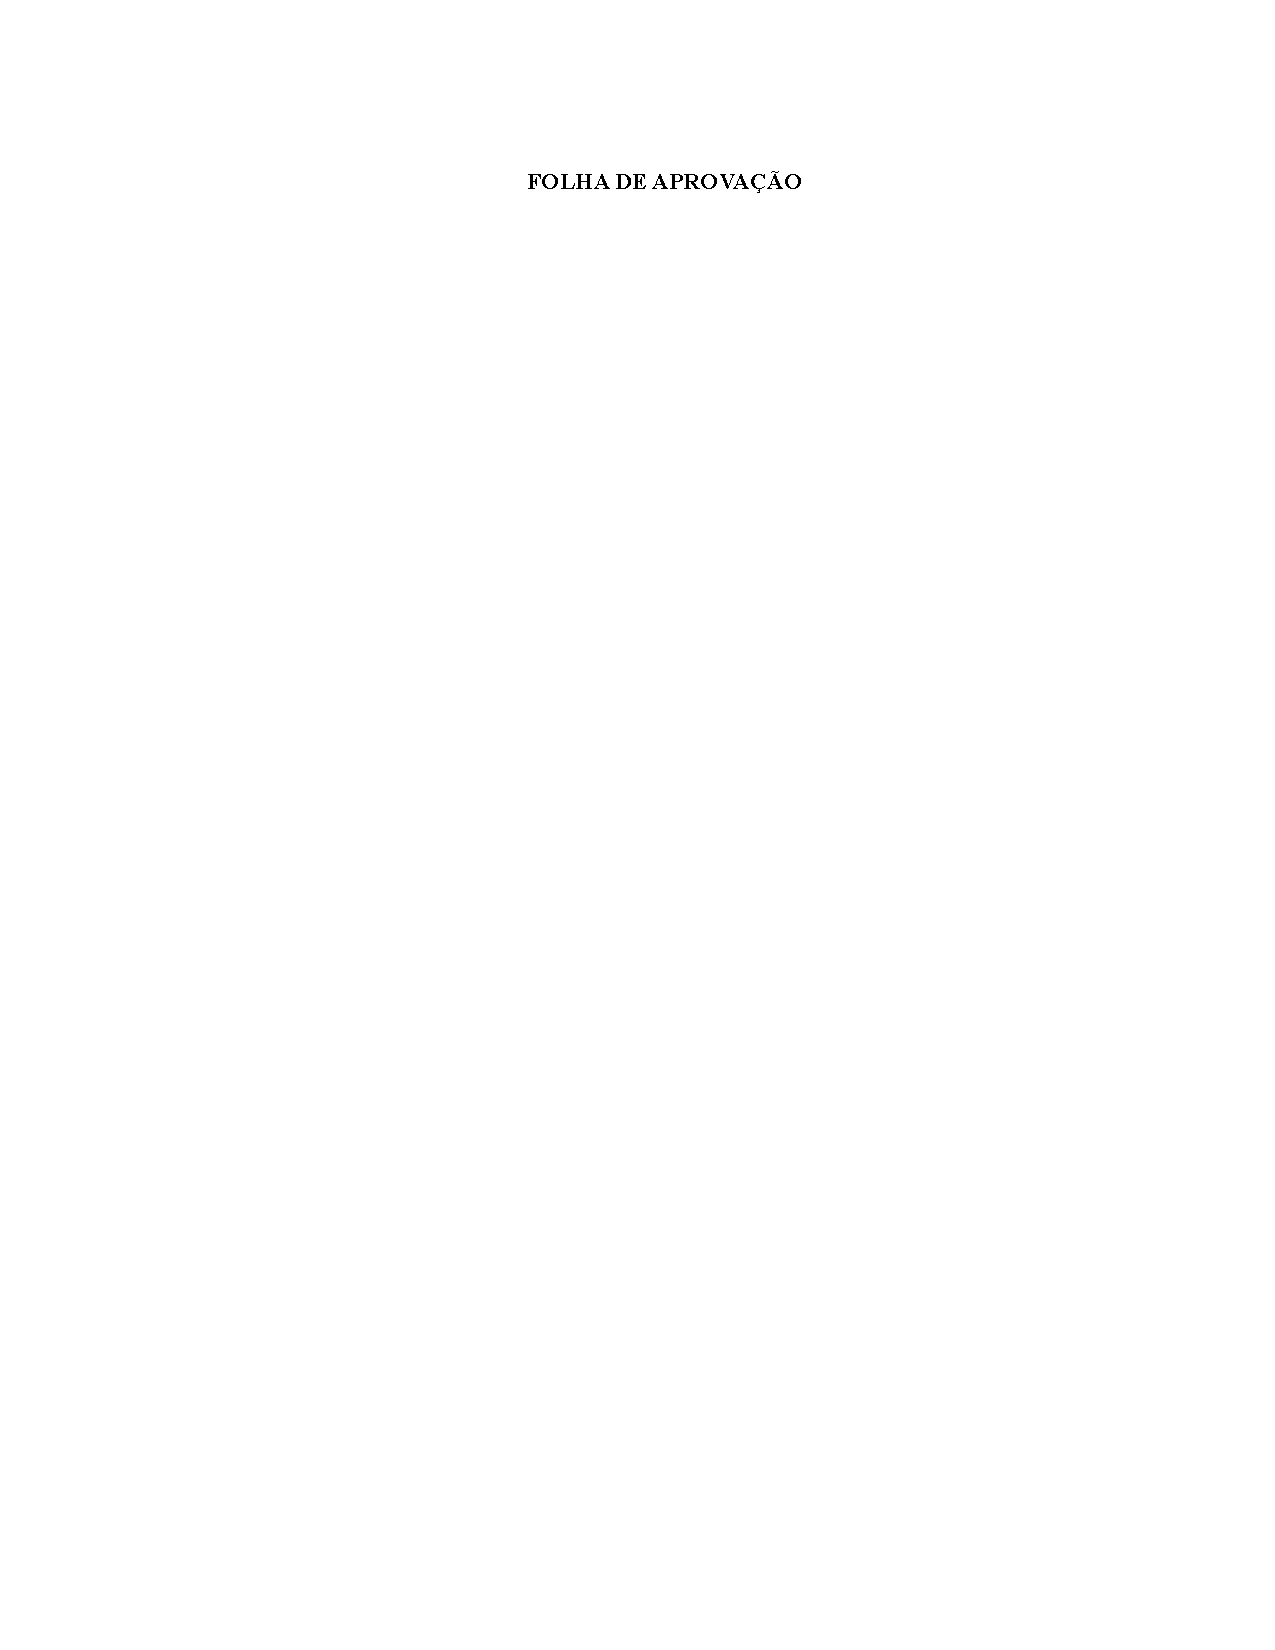
\includepdf[scale=1.0,pages=1]{./PreTexto/folha-aprovacao.pdf} % para adicionar o pdf enviado pelo professor apenas substitua o documento folha-aprovacao.pdf dentro da pasta PreTexto

%% Dedicatória
%%%%% DEDICATÓRIA
%%
%% Texto em que o autor presta homenagem ou dedica seu trabalho.

\begin{dedicatoria}%% Ambiente dedicatoria

%Espaço destinado à dedicatória (elemento opcional). Folha que contém o oferecimento do trabalho à determinada pessoa ou pessoas. Exemplo:



Dedico este trabalho à minha família, pelos momentos de ausência.

\end{dedicatoria}
%% Comente para remover este item

%% Agradecimentos
%%%%% AGRADECIMENTOS
%%
%% Texto em que o autor faz agradecimentos dirigidos àqueles que contribuíram de maneira relevante à elaboração do trabalho.

\begin{agradecimentos}%% Ambiente agradecimentos

Certamente estes parágrafos não irão atender a todas as pessoas que fizeram parte dessa importante fase de minha vida. Portanto, desde já peço desculpas àquelas que não estão presentes entre essas palavras, mas elas podem estar certas que fazem parte do meu pensamento e de minha gratidão. 

Agradeço ao(a) meu(minha) orientador(a) Prof.(a) Dr.(a) Nome Completo, pela sabedoria com que me guiou nesta trajetória.

Aos meus colegas de sala.

A Secretaria do Curso, pela cooperação.

Gostaria de deixar registrado também, o meu reconhecimento à minha família, pois acredito que sem o apoio deles seria muito difícil vencer esse desafio. 

Enfim, a todos os que por algum motivo contribuíram para a realização desta pesquisa.

%Espaço destinado aos agradecimentos (elemento opcional). Folha que contém manifestação de reconhecimento a pessoas e/ou instituições que realmente contribuíram com o(a) autor(a), devendo ser expressos de maneira simples. Exemplo:

%Não devem ser incluídas informações que nominem empresas ou instituições não nominadas no trabalho.

%Se o aluno recebeu bolsa de fomento à pesquisa, informar o nome completo da agência de fomento. Ex: Capes, CNPq, Fundação Araucária, UTFPR, etc. Incluir o número do projeto após a agência de fomento. Este item deve ser o último.

%Atenção: não utilizar este exemplo na versão final. Use a sua criatividade!


\end{agradecimentos}
%% Comente para remover este item

%% Epígrafe
%%%%% EPÍGRAFE
%%
%% Texto em que o autor apresenta uma citação, seguida de indicação de autoria, relacionada com a matéria tratada no corpo do
%% trabalho.

\begin{epigrafe}%% Ambiente epigrafe
%
%Espaço destinado à epígrafe (elemento opcional). Nesta folha, o(a) autor(a) usa uma citação, seguida de indicação de autoria e ano, relacionada, preferencialmente, com o assunto tratado no corpo do trabalho. A citação deverá constar na lista de referências. Exemplo: 
%
``A biblioteca é um jardim onde as ideias florescem e os frutos são colhidos pela eternidade.'' \cite{Candido2002}.
\end{epigrafe}
%% Comente para remover este item

%% Resumo
%%%%% RESUMO
%%
%% Apresentação concisa dos pontos relevantes de um texto, fornecendo uma visão rápida e clara do conteúdo e das conclusões do
%% trabalho.

\begin{resumoutfpr}%% Ambiente resumoutfpr
O resumo deve ressaltar de forma sucinta o conteúdo do trabalho, incluindo justificativa, objetivos, metodologia, resultados e conclusão. Deve ser redigido em um único parágrafo, justificado, contendo de 150 até 500 palavras. Evitar incluir citações, fórmulas, equações e símbolos no resumo. A referência no resumo é elemento opcional em trabalhos acadêmicos, sendo que na UTFPR adotamos por não incluí-la nos resumos contidos nos próprios trabalhos. As palavras-chave e as keywords são grafadas em inicial minúscula quando não forem nome próprio ou nome científico e separados por ponto e vírgula.
\end{resumoutfpr}

%De acordo com a NBR 6028:2021, a apresentação gráfica deve seguir o padrão do documento no qual o resumo está inserido. Para definição das palavras-chave (e suas correspondentes em inglês no abstract) consultar em Termo tópico do Catálogo de Autoridades da Biblioteca Nacional, disponível em: http://acervo.bn.gov.br/sophia_web/autoridade%% Comente para remover este item

%% Abstract
%%%%% ABSTRACT
%%
%% Versão do resumo para idioma de divulgação internacional.

\begin{abstractutfpr}%% Ambiente abstractutfpr
Seguir o mesmo padrão do resumo, com a tradução do texto do resumo e referência, se houver, para a língua estrangeira (língua inglesa).
\end{abstractutfpr}
%% Comente para remover este item

%% Lista de algoritmos
%\incluirlistadealgoritmos%% Comente para remover este item


%% Lista de Ilustrações
%% Figuras, Gráficos, Quadros e Fotografias são incluídos juntos em uma mesma lista
%% Na UTFPR sugere-se adotar listas próprias, conforme a natureza da ilustração, a partir da existência de 3 elementos da mesma natureza.Neste caso, cada lista deverá iniciar em folha distinta. Não criar listas com apenas um item.


%\incluirlistadeilustracoes


%% Lista de figuras
%\incluirlistadefiguras%% Comente para remover este item

%\incluirlistageraldeilustracoes
%\listofgeneralilust



%% Lista de Fotografias
%\incluirlistadefotografias %% Comente para remover este item


%% Lista de Gráficos
%\incluirlistadegraficos %% Comente para remover este item

%% Lista de tabelas
%\incluirlistadetabelas%% Comente para remover este item

%% Lista de quadros
%\incluirlistadequadros

%% Listagem de códigos fonte
%\incluirlistadecodigosfonte

%% Lista de abreviaturas, siglas e acrônimos
\incluirlistadeacronimos{glossaries}%% Opções: "glossaries" (pacote) ou "file" (arquivo) ou "none" (desabilita)

%% Lista de símbolos
%\incluirlistadesimbolos{file}%% Opções: "nomencl" (pacote) ou "file" (arquivo) ou "none" (desabilita)

%% Sumário
\incluirsumario%% Comente para remover este item

%% Formatação de páginas de elementos textuais
\textual%% Não comente esta linha

%% Parte
% \part{Introdução}%% Comente para remover este item

%% Capítulo introdução - obrigatório
%%%% CAPÍTULO 1 - INTRODUÇÃO
%%
%% Deve apresentar uma visão global da pesquisa, incluindo: breve histórico, importância e justificativa da escolha do tema,
%% delimitações do assunto, formulação de hipóteses e objetivos da pesquisa e estrutura do trabalho.

%% Título e rótulo de capítulo (rótulos não devem conter caracteres especiais, acentuados ou cedilha)

\chapter{Introdução}\label{cap:introducao}

\caixa{Deve conter algum conteúdo}{Ler tese do professor para inspiração}

\section{Tema}

\caixa{Deve conter algum conteúdo}{Elabore um parágrafo, dois ou três, no máximo, descrevendo a linha do tempo em que as indústrias começaram com os paradigmas (rótulos) .0, .2, .3, …, até a indústria 4.0 (Da onde vem esta nomenclatura). Daí, estabelece-se o gancho para o próximo parágrafo. 
Neste contexto, é importante ressaltar a questão histórica, apresentando de forma resumida as características principais de cada uma delas no tempo.}

A Indústria 5.0 representa a evolução do paradigma da Indústria 4.0, estendendo o foco exclusivo na automação e eficiência operacional para integrar dimensões socioeconômicas.
Esse novo paradigma industrial prioriza a colaboração entre humanos e máquinas e está centrada na busca da valorização da criatividade humana.
Dessa forma, desenvolvendo ambientes de trabalho mais saudáveis, estimulando o trabalho criativo e colaborativo, bem como integrando valores éticos e sociais aos processos industriais.
Os outros pilares da Indústria 5.0 incluem sustentabilidade e resiliência utilizando a tecnologia como meio de ampliar as capacidades humanas.
% \cite{euCommission2021,Xu2021}.

O conceito "Indústria 5.0" ganhou destaque em documentos estratégicos da União Européia desenvolvidos por \citeonline{euCommission2021}, que enfatizam a necessidade de sistemas industriais resilientes, sustentáveis e centrados nas pessoas.
Essa mudança de modelo industrial reflete o reconhecimento de que desafios contemporâneos, como mudanças climáticas, envelhecimento populacional e escassez de recursos, exigem um modelo de produção mais sensível às necessidades humanas e ambientais.

A proposta da Indústria 5.0 envolve um redesenho do sistema produtivo, no qual a tecnologia é utilizada como meio para potencializar as capacidades humanas, promovendo um ambiente de produção que integre valores éticos às operações industriais.
Esse novo paradigma demanda transformações organizacionais profundas, deslocando o foco exclusivo da produtividade para a criação de valor social. % \cite{HeinPensel2023}

Nesse contexto, torna-se necessário avaliar em que medida as organizações estão prontas para essa transformação.
A mensuração do grau de maturidade organizacional frente à Indústria 5.0 possibilita identificar lacunas estruturais, definir diretrizes de transformação e orientar políticas industriais.
A maioria dos modelos de avaliação de maturidade existentes ainda se fundamenta nas premissas da Indústria 4.0, priorizando a maturidade tecnológica e negligenciando dimensões como sustentabilidade e ética digital \cite{Lucato2019,HeinPensel2023}.
Assim, surge a necessidade de instrumentos mais aderentes à realidade da Indústria 5.0.
\citeonline{HeinPensel2023} realizaram uma revisão sistemática da literatura e identificaram que, embora existam diversos modelos de maturidade voltados à Indústria 4.0, a maioria negligencia os pilares essenciais como bem-estar dos trabalhadores, inclusão social e responsabilidade ambiental.
Por isso, a avaliação de maturidade nesse novo cenário apresenta desafios como a ausência de modelos consolidados, critérios qualitativos subjetivos e a coexistência com elementos contraditórios.

Além disso, o modelo proposto por \citeonline{BARO2025}, fundamentado na Teoria Sociotécnica desenvolvida por \citeonline{Trist1981}, representa um avanço ao integrar quatro perspectivas interdependentes: estratégia sistêmica, sustentabilidade, centralidade no ser humano e resiliência.
\caixa{TO DO}{Definir termo abordagem holística}
Essa abordagem holística oferece a granularidade necessária para traduzir os princípios de alto nível da Indústria 5.0 e da Teoria Sociotécnica em um modelo estruturado e permite que as organizações avaliem seu estado atual de implementação da Indústria 5.0 e alinhem suas estratégias com suas capacidades, recursos e objetivos atuais.
Além disso, os autores destacam a escassez de modelos práticos e a necessidade de desenvolvimento de ferramentas de diagnóstico que considerem os fatores humanos e sociais como fatores essenciais do processo de avaliação de maturidade.

Um instrumento diagnóstico capaz de representar e processar informações contraditórias, permitindo, assim, capturar a complexidade sociológica desse novo paradigma industrial, pode ser representado pela Lógica Paraconsistente.
Esta aboradagem lógica permite a tomada de decisões mesmo diante de inconsistências ou dados conlfitantes.Existem aplicações da lógica paraconsistente /TODO em sistemas de controle, inteligência artificial e diagnósticos, especialmente na área médica, demonstram sua robustez frente a incertezas e contradições \cite{SilvaFilho1999, CarvalhoBrunsteinAbe2003, CarvalhoJunior2024}.

\caixa{TO DO}{Ler Tese do professor para inspiração em relação ao uso de citações diretas}
 
\caixa{TO DO}{Tratar do encadeamento dos assuntos no subtítulo Tema}


\section{Delimitação do Tema}

A presente pesquisa concentra-se no desenvolvimento de um instrumento diagnóstico para a avaliação de maturidade da Indústria 5.0, com um recorte metodológico específico na aplicação da \gls{LPA2v}.
O escopo do trabalho abrange a definição dos critérios de avaliação alinhados aos pilares da Indústria 5.0, a estruturação de um algoritmo de análise baseado na \gls{LPA2v} e o desenvolvimento de um instrumento diagnóstico.
Restringir a metodologia ao uso da \gls{LPA2v}, visa explorar sua capacidade de representar critérios muitas vezes subjetivos ou contraditórios, como bem-estar dos trabalhadores ou equilíbrio entre automação e autonomia humana.
Diversos estudos mostram que os modelos de maturidade atuais, mesmo os que começam a considerar a Indústria 5.0, ainda carecem de instrumentos formais capazes de lidar com a complexidade socio-técnica desse novo paradigma \cite{BARO2025, HeinPensel2023}.
Assim, propõe-se investigar a suficiência da \gls{LPA2v} como base para representação e análise da maturidade organizacional em termos dos pilares da Indústria 5.0 como human-centricidade, sustentabilidade e resiliência.

\section{Problema}
\caixa{TO DO}{Ler a seção da tese do professor. Lembrando que o problema tem que terminar com a pergunta da pesquisa}

Os instrumentos atualmente disponíveis para avaliação de maturidade organizacional foram concebidos majoritariamente sob a lógica da Indústria 4.0 e permanecem centrados em critérios técnico-operacionais.
Essa lacuna é evidenciada por \citeonline{HeinPensel2023}, que mostram que poucos modelos existentes contemplam dimensões qualitativas cruciais da Indústria 5.0, como bem-estar dos trabalhadores, ética digital e impacto socioambiental.

Neste cenário, a \gls{LPA2v} apresenta-se como uma alternativa formal viável para representar esses estados de evidência conflitante, viabilizando análises diagnósticas mesmo sob condições de incerteza \cite{JoseSilvaFilho2006, CarvalhoBrunsteinAbe2003, CarvalhoJunior2024}.
No entanto, observa-se que ainda não existem modelos específicos de avaliação diagnóstica da maturidade em Indústria 5.0 fundamentados na \gls{LPA2v}.
Dessa forma, discutimos a aplicação da \gls{LPA2v} para desenvolver um instrumento diagnóstico capaz de avaliar os níveis de maturidade de uma organização frente às dimensões da Indústria 5.0.

\section{Objetivos}

\subsection{Objetivo Geral}

Desenvolver um instrumento diagnóstico, utilizando a \gls{LPA2v}, para avaliação dos níveis de maturidade da Indústria 5.0 em organizações industriais.

\subsection{Objetivos Específicos}

\begin{itemize}
  \item Revisar os modelos de avaliação de maturidade existentes tanto para a Indústria 4.0 quanto para indústria 5.0;
  \item Identificar e estruturar os critérios e dimensões relevantes para diagnóstico de maturidade na Indústria 5.0;
  \item Modelar os critérios e dimensões selecionados utilizando a \gls{LPA2v};
  \item Propor um algoritmo para-analisador, baseado em \gls{LPA2v}, capaz de interpretar e classificar os níveis de maturidade.
  \item Aplicar o modelo proposto em um estudo de caso, validando sua capacidade de gerar diagnósticos sob condições de incerteza e contradição;
\end{itemize}

\section{Justificativa}

Como a \gls{LPA2v} é capaz  de lidar formalmente com incertezas e contradições, o modelo proposto busca suprir uma lacuna metodológica e atender à demanda por ferramentas avaliativas mais alinhadas aos novos princípios industriais.
A contribuição esperada é tanto teórica, expandindo o campo de aplicação da \gls{LPA2v}, quanto prática, ao oferecer um modelo aplicável em contextos organizacionais reais que buscam se alinhar às diretrizes da emergente Indústria 5.0.

\section{Metodologia}

A metodologia proposta neste trabalho está organizada em quatro etapas principais:
\begin{enumerate}[label=\roman*.]
    \item Revisão da literatura e definição das dimensões de análise
    \item Estruturação do modelo avaliativo utilizando a \gls{LPA2v}
    \item Aplicação do modelo em uma organização industrial
    \item Avaliação dos resultados e da aplicabilidade do modelo proposto
\end{enumerate}

Na primeira etapa, será realizada uma revisão sistemática da literatura com o objetivo de identificar os critérios qualitativos relevantes para compor um diagnóstico de maturidade voltado à Indústria 5.0.
Serão consideradas dimensões alinhadas aos pilares desse novo paradigma, como centralidade no ser humano, sustentabilidade, ética digital e resiliência organizacional \cite{euCommission2021}.

Com base nas dimensões identificadas, será estruturado um conjunto de fatores de influência, que representam as principais variáveis intervenientes na determinação do nível de maturidade.
Esses fatores serão organizados em seções em que cada uma corresponde a um domínio conceitual da Indústria 5.0. 

Em seguida, o modelo será aplicado a partir de avaliações realizadas por especialistas do contexto analisado, os quais atribuirão, para cada fator, os pesos relativos e os graus de evidência favorável ($\mu_1$) e desfavorável ($\mu_2$).
Após a coleta dos dados e definição do nível de exigência, os resultados obtidos serão interpretados considerando os graus de certeza e contradição. Por fim, avalia-se a capacidade do modelo em produzir diagnósticos consistentes.

\section{Estrutura do Trabalho}

Este trabalho está organizado em cinco capítulos, conforme descrito a seguir:

\begin{itemize}
    \item \textbf{Capítulo 1- Introdução}: Apresenta o tema de estudo, sua delimitação do tema, o problema de pesquisa, os objetivos geral e específicos, a justificativa, a metodologia adotada e a estrutura geral da pesquisa acadêmica.
    
    \item \textbf{Capítulo 2 - Indústria 5.0}: Trata da fundamentação teórica sobre a Indústria 5.0, destacando seus pilares conceituais e a necessidade de abordagens diagnósticas mais alinhadas a esse novo paradigma.
    
    \item \textbf{Capítulo 3 - Lógica Paraconsistente}: Apresenta a \gls{LPA2v}, incluindo a metodologia a ser utilizada para avaliação diagnóstica.
    
    \item \textbf{Capítulo 4 - Modelo de Avaliação Diagnóstica}: Propõe a aplicação e análise do método paraconsistente de decisão para avaliação diagnóstica de maturidade organizacional frente à Indústria 5.0.
    Este capítulo descreve a criação do modelo, os fatores de influência utilizados, a análise dos resultados obtidos após a aplicação do modelo.
    
    \item \textbf{Capítulo 5 - Conclusões e Considerações finais}: Apresenta as considerações finais do trabalho as limitações da abordagem desenvolvida e sugestões para estudos futuros que possam aprimorar ou expandir o modelo proposto.
\end{itemize}

\begin{comment}
\noindent Exemplos de citação:

Segundo \citeonline{Coulouris2013}.

Segundo \citeonline[p. 40]{Coulouris2013}.

Citação no final do Parágrafo~\cite{Coulouris2013}. 

Citação no final do Parágrafo com número de página~\cite[p. 40]{Coulouris2013}.

%(Modelo de referência: pessoa jurídica)
Citação no final do Parágrafo~\cite{NBR6023:2018}

%(Modelo de referência: pessoa jurídica)
Citação no final do Parágrafo~\cite{NBR6027:2012}

%(Modelo de referência: pessoa jurídica)
Citação no final do Parágrafo~\cite{NBR6028:2021}

Segundo a \citeonline{NBR14724:2011}.

Citação no final do Parágrafo~\cite{NBR10520:2002}

Citação no final do Parágrafo~\cite{NBR14724:2011}.

% (Modelo de referência de trabalho acadêmico).
Citação no final do Parágrafo~\cite{Andrade2005}

% (Modelo de referência: capítulo de livro).
Citação no final do Parágrafo~\cite{Borges2014}

% (Modelo de referência: leis, decretos, portarias, etc.)
Citação no final do Parágrafo~\cite{BRASIL:1998}

% (Modelo de referência: livro com subtítulo). Nome com sufixo "Von" - Configuração no bib
Citação no final do Parágrafo~\cite[p. 66]{KROGH:2001}

Citação no final do Parágrafo~\cite{Faina2001}

% (Modelo de referência: livro com subtítulo).
Citação no final do Parágrafo~\cite{Davenport2012}

% (Modelo de referência: artigo de periódico).
Citação no final do Parágrafo~\cite{Monteiro2009}

%(Modelo de referência: artigo de periódico). Nome familiar "Junior"
Citação no final do Parágrafo~\cite{Sanches2024}

% (Modelo de referência: trabalho publicado em evento).
Citação no final do Parágrafo~\cite{Renaux2001}

Em relação ao assunto, o apresentado nesta seção pode estar relacionado a trabalhos de outros autores ou ao assunto que fornece a fundamentação (motivação) para o trabalho a ser desenvolvido. Se o assunto está relacionado a trabalhos de outros autores, a contribuição do trabalho é definida em relação ao que já foi pesquisado nesse assunto. Se o assunto será utilizado para embasamento do que será proposto, explicitar como o trabalho se insere nesse assunto. A contribuição pode, ainda, estar relacionada a uma necessidade de mercado ou a uma oportunidade decorrente de algum problema real para o qual se pretender propor uma solução. Nesse caso, o assunto fornece um contexto teórico de suporte para o problema e/ou a solução.

O importante nesta seção é deixar claro do que se trata o trabalho (assunto ou tema), identificar o objeto de pesquisa, como será encaminhada a solução (procedimento metodológico, tecnologias, ferramentas utilizadas) e o que se pretende ao final do trabalho, sem explicitar a solução e os resultados.



\begin{photograph}[!htb]%% Ambiente figure
    %\captionsetup{width=0.55\textwidth}%% Largura da legenda
    \caption{Exemplo de fotografia}%% Legenda
    \label{fig:exemplo1}%% Rótulo
    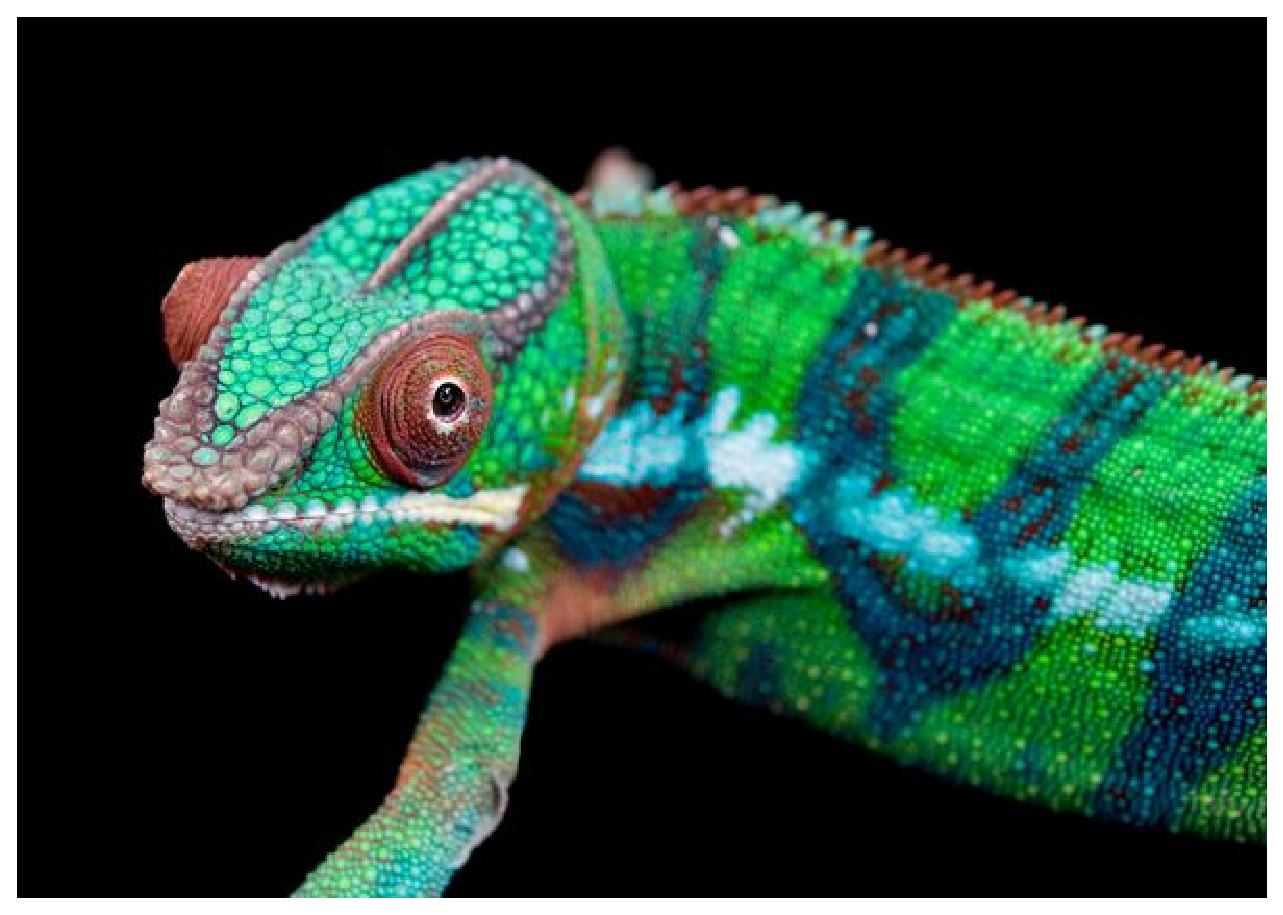
\includegraphics[scale=0.4]{foto1}%% Dimensões e localização
    \fonte{Autoria Própria}%% Fonte
    \addcontentsline{loge}{photograph}{\protect\numberline{\thephotograph}Exemplo de fotografia.} % Adiciona à lista de ilustrações
\end{photograph}

Os objetivos específicos são opcionais, ou seja, somente devem ser apresentados se caracterizarem resultados parciais gerados a partir do objetivo geral, os quais sejam considerados úteis para a comunidade acadêmica, para a sociedade ou para o ambiente profissional. Uma observação importante é que os resultados sejam passíveis de comprovação, ou seja, se o objetivo for: “Oferecer agilidade e confiabilidade aos processos gerenciais da empresa”, significa que o trabalho deverá realizar testes com relação a esses atributos, cujos resultados deverão ser apresentados nas discussões do trabalho.

\begin{graph}[!htb]%% Ambiente figure
    %\captionsetup{width=0.55\textwidth}%% Largura da legenda
    \caption{Exemplo de gráfico}%% Legenda
    \label{graph1}%% Rótulo
    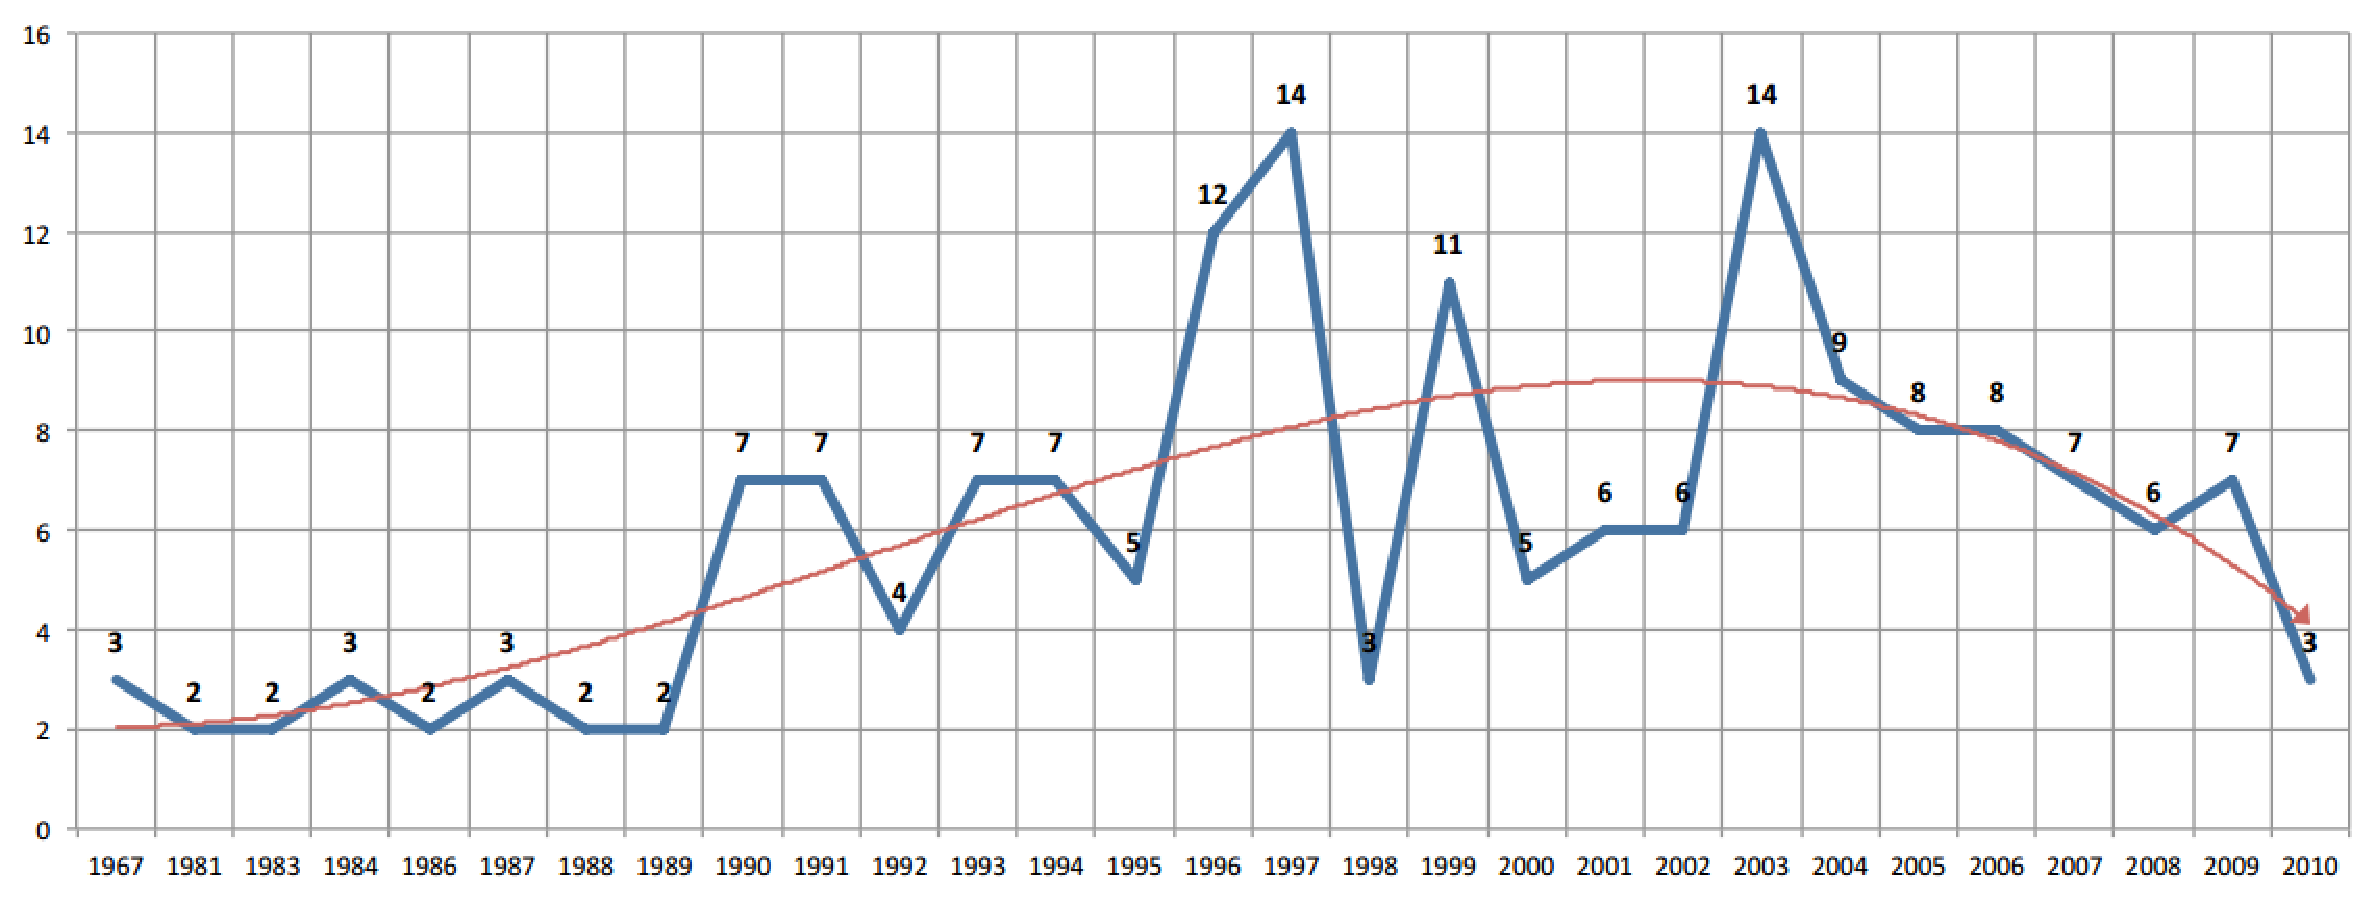
\includegraphics[scale=0.4]{grafico2}%% Dimensões e localização
    \fonte{Adaptado de \citeonline[p.~4]{UTFPR2008}}%% Fonte
    \addcontentsline{loge}{graph}{\protect\numberline{\thegraph}Exemplo de gráfico.}
\end{graph}


Destaca-se que os objetivos específicos não incluem as etapas do processo de desenvolvimento de software (realizar a modelagem, a análise, o projeto...) ou outras atividades necessárias para alcançar o objetivo geral, como, estudar as tecnologias necessárias para modelagem e implementação do sistema. Dentre as exceções estão a realização de estudos, procedimentos, métodos e técnicas considerados inéditos e de relevância para outros trabalhos a serem realizados na mesma área. Contudo, o resultado deste estudo deve ser documentado de forma que seja conhecimento disponibilizado para quem lê o trabalho.


\subsection{Seção ternária (sublinhado)}

xxxxxxxx mkmdasda

asdadas

 
\subsubsection{Seção quaternária (sublinhado)}

xxxxxxxxx

dasda

\subsubsubsection{Seção quinária (itálico)}
\end{comment}
\begin{comment}
Justificar o objeto de pesquisa (o que será feito) e a forma de resolução do problema (como fazer). A forma de resolução pode estar centrada no método, nas tecnologias, no uso de conceitos (fundamentação teórica).

A Justificativa explicita porque desenvolver o referido trabalho, como o mesmo se insere no contexto de pesquisa, de produção científica. Pode incluir o porquê utilizar as tecnologias e ferramentas indicadas, a contribuição em termos de inovação ou mesmo de aprendizado.

O trabalho não precisa ser justificado em decorrência de ser inovador ou por ter gerado uma significativa contribuição ao conhecimento na área em que o mesmo se insere. Pode referir-se simplesmente à aplicabilidade de conhecimentos adquiridos durante o curso. Sendo assim, a justificativa não deve ser elaborada considerando um mercado a ser atingido e sim com relação ao uso de tecnologias aprendidas e/ou estudadas, o conhecimento e aprendizado do aluno e a aplicabilidade do trabalho desenvolvido.
\end{comment}
\begin{comment}
A estrutura do trabalho contém uma relação dos capítulos e uma descrição sucinta do que cada um deles contém. Esta seção fornece uma visão geral do trabalho no sentido da sua estrutura em capítulos\footnote{Teste de nota de rodapé 2.}.

\caixa{Atenção}{O OverLeaf está demorando muito para compilar o modelo com o Capítulo de Exemplos, que explica como usar o LaTeX. Assim, esse capítulo foi removido (está comentado para não compilar), mas há um arquivo chamado \texttt{exemploPDF.pdf}, na raiz do projeto, que contém esse capítulo de exemplos!}
\end{comment}






%% Comente para remover este item

%% Capítulo 1 da fundamentação teórica
%%%% CAPÍTULO 2 - REVISÃO DA LITERATURA (OU REVISÃO BIBLIOGRÁFICA, ESTADO DA ARTE, ESTADO DO CONHECIMENTO)
%%
%% O autor deve registrar seu conhecimento sobre a literatura básica do assunto, discutindo e comentando a informação já publicada.
%% A revisão deve ser apresentada, preferencialmente, em ordem cronológica e por blocos de assunto, procurando mostrar a evolução do tema.
%% Título e rótulo de capítulo (rótulos não devem conter caracteres especiais, acentuados ou cedilha)

\chapter{Indústria 5.0}\label{cap:indutria5_0}
\section{Histórico das Revoluções Industriais}

As transformações industriais ao longo da história moldaram a estrutura produtiva da sociedade.
A Primeira Revolução Industrial, no final do século XVIII, foi impulsionada pela energia a vapor, marcando a transição da produção manual para o modelo fabril mecanizado.
A Segunda Revolução Industrial, no século XIX, trouxe a eletricidade e a produção em massa, elevando drasticamente a produtividade.
A Terceira Revolução Industrial, a partir da década de 1970, integrou eletrônica, automação e tecnologias da informação e comunicação, levando à produção automatizada.
A Quarta Revolução Industrial, ou Indústria 4.0, focou na interconectividade de sistemas físicos e digitais, utilizando tecnologias como \gls{IoT} e computação em nuvem e inteligência artificial \cite{VALETTE2023}.
Essa fase da revolução industrial buscou automação avançada, decisões autônomas e customização em massa.
Contudo, a Indústria 4.0 foi criticada por sua abordagem predominantemente tecnológica, negligenciando aspectos humanos, sociais e ambientais dos sistemas produtivos.
Essa falha na aboradagem abriu caminho para o surgimento da Indústria 5.0, que busca reintroduzir valores como a centralidade humana, a sustentabilidade e a resiliência \cite{Xu2021, PIZON2023}.
\caixa{TO DO}{Remover esse trecho e adicionar ao tema. Verificar a possibilidade de citações diretas}

\section{Limitações da Indústria 4.0}

\caixa{TO DO}{Incluir citações diretas em relação as limitações da indústria 5.0}
A Indústria 4.0, embora tenha impulsionado a eficiência e a produtividade por meio da digitalização e automação, tem sido criticada por sua abordagem predominantemente tecnológica, que muitas vezes negligencia os aspectos humanos, sociais e ambientais dos sistemas produtivos.
A marginalização do papel do trabalhador é uma das principais limitações, com sistemas de planejamento e controle que priorizam a automação em detrimento de fatores cognitivos e perceptivos humanos \cite{RANNERTSHAUSER2022}.
Além disso, a Indústria 4.0 apresenta lacunas em relação à sustentabilidade e resiliência. Apesar dos ganhos de produtividade, seu modelo tecnológico não considerou a preservação ambiental e a capacidade de adaptação a crises sistêmicas, como evidenciado pela pandemia de COVID-19 \cite{euCommission2021, Khan2023}.

Diante desses desafios, a Indústria 5.0 surge como uma evolução que busca resgatar o protagonismo humano e ampliar o foco para além da eficiência econômica.
O objetivo é criar sistemas produtivos que não apenas automatizam tarefas, mas que também fortaleçam a criatividade, a personalização e a inclusão.
Essa mudança de enfoque está fundamentada em três pilares centrais: centralidade no ser humano, sustentabilidade ambiental e resiliência organizacional \cite{euCommission2021, Nahavandi2019}.

\section{Modelo da Indústria 5.0}

A Indústria 5.0 representa uma evolução do modelo industrial, transcendendo o foco exclusivo na eficiência e produtividade da Indústria 4.0 para incorporar valores como a centralidade no ser humano, a sustentabilidade e a resiliência \cite{euCommission2021, Xu2021}.
Essa nova fase da indústria busca harmonizar o avanço tecnológico com o bem-estar social e a proteção ambiental \cite{Nahavandi2019}.

A centralidade no ser humano implica em um redesenho dos sistemas produtivos onde o trabalhador é visto como um ativo valioso e não apenas como um custo.
A tecnologia deve servir para ampliar as capacidades humanas, promover ambientes de trabalho seguros e inclusivos, e garantir que as decisões sejam tomadas com consideração ética e respeito à dignidade humana \cite{Nahavandi2019, TOTH2023}.
Isso se manifesta na colaboração humano-máquina, onde robôs e sistemas de IA atuam como assistentes, potencializando a criatividade e o julgamento humano em tarefas complexas \cite{VALETTE2023}.

A sustentabilidade, por sua vez, orienta a Indústria 5.0 para a criação de processos produtivos que respeitem os limites planetários.
Isso envolve a adoção de tecnologias verdes, a promoção da economia circular, a redução do consumo de energia e recursos, e a minimização de resíduos e emissões.
O objetivo é garantir que a produção industrial contribua para um futuro mais verde e equitativo, alinhando o desenvolvimento econômico com a responsabilidade ambiental \cite{euCommission2021, silva2024}.

A resiliência é o terceiro pilar, capacitando as indústrias a resistirem e se adaptarem a choques e interrupções, como crises geopolíticas, pandemias ou desastres naturais.
Isso requer cadeias de suprimentos mais robustas e flexíveis, capacidade de produção adaptável e processos de negócios ágeis.
A Indústria 5.0 busca construir sistemas que possam manter sua funcionalidade e se recuperar rapidamente diante de adversidades, garantindo a continuidade das operações essenciais \cite{euCommission2021, Khan2023}.

Em suma, a Indústria 5.0 não é uma substituição da Indústria 4.0, mas um complemento que adiciona uma dimensão de valores, focando em como a tecnologia pode ser utilizada para alcançar objetivos sociais e ambientais mais amplos, além dos ganhos de eficiência.
Ela representa uma mudança de paradigma de uma abordagem puramente tecnológica para uma abordagem orientada por valores, onde a inovação e a pesquisa são direcionadas para o serviço à humanidade dentro dos limites planetários \cite{Xu2021, VALETTE2023}.

\section{Indicadores e Métricas da Indústria 5.0}

A mensuração do progresso em direção à Indústria 5.0 requer a formulação de indicadores que ultrapassem os tradicionais parâmetros técnico-econômicos da Indústria 4.0.
Isso implica considerar dimensões como centralidade no ser humano, sustentabilidade e resiliência organizacional \cite{euCommission2021, Nahavandi2019}.
Ao contrário da Indústria 4.0, que priorizava a eficiência operacional, a Indústria 5.0 demanda um novo conjunto de métricas capazes de captar aspectos qualitativos e contextuais.
Indicadores como tempo de ciclo das máquinas ou taxa de falhas continuam relevantes, mas são complementados por medidas subjetivas, como bem-estar dos trabalhadores, aceitação da IA e confiança nos sistemas \cite{TOTH2023}.

Autores como \citeonline{TOTH2023} propõem a arquitetura colaborativa I5arc, que organiza os indicadores da Indústria 5.0 em seis domínios de melhoria contínua, com base em processos colaborativos entre humanos, inteligência artificial e sistemas ciberfísicos.


\section{Relação entre Sociedade 5.0 e Indústria 5.0}

A Sociedade 5.0, um conceito originado no Japão, representa uma visão de futuro na qual a transformação digital é orientada para o bem-estar social, integrando o mundo físico e o ciberespaço para resolver desafios sociais por meio da tecnologia.
Enquanto a Sociedade 5.0 abrange amplos setores como educação, mobilidade, saúde e segurança, a Indústria 5.0 aplica princípios semelhantes ao contexto produtivo, focando na reorganização dos sistemas de manufatura com base em valores \cite{Santos2025,Xu2021}.

Ambos os conceitos compartilham a centralidade no ser humano, a sustentabilidade e a valorização da tecnologia como meio para um fim social, e não como um fim em si mesma.
No entanto, operam em escalas e escopos distintos: a Sociedade 5.0 é uma estratégia nacional abrangente, dependente de políticas públicas e ações coordenadas entre governos, universidades e sociedade civil.
Já a Indústria 5.0 é um desdobramento setorial, que exige o redesenho de práticas organizacionais e modelos de gestão específicos para o ambiente fabril \cite{PIZON2023, TOTH2023}.

A Indústria 5.0 pode ser vista como uma interface operacional da Sociedade 5.0 no domínio industrial, buscando personalização, sustentabilidade e resiliência dentro dos sistemas de produção.
Essa convergência dentro dos sistemas de produção indica uma tendência de evolução sistêmica, onde tecnologia, sociedade e indústria caminham juntas para promover não apenas avanços técnicos, mas também valor social agregado, superando as limitações dos modelos anteriores que priorizavam apenas a eficiência econômica \cite{VALETTE2023}.

\section{Pilares da Indústria 5.0}

\caixa{TO DO}{(Gostaria que você já destacasse os Fatores de Influência em cada um dos pilares}

\subsection{Centralidade no ser humano}

A centralidade no ser humano é um dos pilares fundamentais da Indústria 5.0, diferenciando-a da Indústria 4.0, que focava na automação e digitalização para ganhos de produtividade.
A Indústria 5.0 propõe um redesenho dos sistemas industriais com ênfase na valorização das capacidades humanas, na sustentabilidade e na resiliência dos processos produtivos \cite{VALETTE2023, euCommission2021}.

Essa abordagem foca no ser humano e objetiva resgatar o papel ativo do operador nos ambientes fabris, não apenas como executor, mas como cocriador e agente decisório.
A literatura aponta a necessidade de sistemas colaborativos entre humanos, inteligência artificial e dispositivos ciberfísicos, promovendo uma sinergia entre as capacidades cognitivas humanas e os recursos tecnológicos avançados \cite{TOTH2023, Santana_2023}.
Modelos como o Human-in-the-loop Cyber-Physical Systems e o Operator 4.0 refletem essa tendência, onde o humano permanece no centro das decisões, especialmente em tarefas que exigem criatividade, julgamento moral, sensibilidade contextual e solução de problemas não estruturados \cite{VALETTE2023, RANNERTSHAUSER2022}.

O pilar da centralidade no ser humano também demanda um redesenho das arquiteturas organizacionais e tecnológicas, com a incorporação de dispositivos usáveis, gêmeos digitais, realidade aumentada e tecnologias explicáveis de IA, com interfaces que garantam que o controle permaneça nas mãos dos operadores \cite{TOTH2023, YANG2024}.
A Indústria 5.0 valoriza atributos humanos como criatividade, pensamento crítico, empatia, julgamento ético e adaptabilidade, que são indispensáveis para lidar com problemas não estruturados e interpretar contextos complexos \cite{RANNERTSHAUSER2022, Nahavandi2019}.

O papel do operador vai além da execução de tarefas, esperando-se que ele participe ativamente do processo decisório, proponha melhorias e interaja com sistemas baseados em inteligência artificial de forma ética e explicável \cite{TOTH2023, PIZON2023}.
Além disso, o desenvolvimento de competências emocionais e sociais é essencial para a criação de ambientes industriais inclusivos e saudáveis, promovendo o bem-estar psicológico, a comunicação efetiva e a cooperação entre equipes humanas e agentes tecnológicos \cite{Santana_2023}.
% Ribeiro2024

\subsection{Sustentabilidade}

A sustentabilidade é um dos pilares fundamentais da Indústria 5.0, assumindo uma posição de destaque em relação aos paradigmas industriais anteriores.
Enquanto a Indústria 4.0 concentrou-se na eficiência operacional e na digitalização, muitas vezes sem considerar de forma abrangente os impactos ambientais, a Indústria 5.0 propõe uma abordagem mais equilibrada, na qual o desenvolvimento tecnológico está alinhado à preservação dos recursos naturais e ao respeito aos limites planetários \cite{VALETTE2023, silva2024, Rame2024}.

Segundo a Comissão Europeia, a Indústria 5.0 reconhece a necessidade de sistemas produtivos resilientes e ambientalmente responsáveis, capazes de enfrentar desafios como as mudanças climáticas, a escassez de recursos e a instabilidade nas cadeias globais de suprimentos.
Nesse contexto, o uso de tecnologias verdes torna-se essencial para mitigar os impactos ambientais da produção industrial, promovendo a economia circular e a redução da pegada de carbono \cite{Rame2024}.

As tecnologias verdes envolvem inovações que minimizam o consumo de energia e matérias-primas, reduzem emissões e resíduos e promovem ciclos de produção mais circulares.
Entre os exemplos estão a manufatura aditiva com materiais biodegradáveis, sistemas de recuperação de energia, sensores de eficiência energética, além de processos produtivos orientados por inteligência artificial que otimizam recursos em tempo real \cite{TOTH2023, silva2024}.
A integração da sustentabilidade ao design dos sistemas industriais requer não apenas tecnologias apropriadas, mas também uma reestruturação dos modelos de negócios e métricas de desempenho, vinculando a criação de valor econômico ao impacto social e ecológico das operações industriais \cite{Santos2025}.

\subsection{Resiliência}

A resiliência é um componente estrutural da Indústria 5.0, cuja proposta é capacitar os sistemas industriais a resistirem, adaptarem-se e se recuperarem rapidamente de perturbações internas ou externas.
Em contraste com a Indústria 4.0, que priorizou a eficiência operacional e a hiperconectividade, a Indústria 5.0 enfatiza a capacidade dos sistemas de produção em manter sua funcionalidade diante de eventos adversos, como pandemias, crises geopolíticas, escassez de insumos ou falhas tecnológicas \cite{euCommission2021, VALETTE2023, Khan2023}.

A resiliência industrial envolve a integração de mecanismos técnicos, organizacionais e humanos capazes de detectar vulnerabilidades, responder a falhas e ajustar-se de maneira autônoma ou assistida.
Essa abordagem requer modelos de produção mais flexíveis, redes de suprimentos diversificadas e estruturas organizacionais descentralizadas, com maior autonomia local para tomada de decisão \cite{Santos2025, silva2024}.
Segundo \citeonline{TOTH2023}, a arquitetura colaborativa proposta pela Indústria 5.0 amplia a resiliência ao promover a participação ativa dos trabalhadores em processos de inovação e adaptação contínua, com o apoio de tecnologias inteligentes que fornecem suporte decisório em tempo real.
A presença de humanos no ciclo de controle favorece diagnósticos contextuais mais precisos e respostas mais eficazes frente à incerteza \cite{TOTH2023}.

Além disso, o uso de tecnologias como gêmeos digitais, realidade aumentada, inteligência artificial explicável e sistemas distribuídos permite antecipar riscos, simular cenários e reagir de forma ágil a mudanças imprevistas.
Esses elementos tornam-se cruciais para enfrentar ambientes voláteis, incertos, complexos e ambíguos, especialmente em cadeias globais de valor \cite{VALETTE2023}.
A resiliência na Indústria 5.0 não deve ser compreendida apenas como a capacidade tecnológica de resistir a choques externos, mas como uma propriedade sistêmica construída a partir de arranjos organizacionais, culturais e humanos \cite{TOTH2023, Santos2025}.

Um dos elementos centrais para a resiliência organizacional é a promoção de uma cultura de aprendizado contínuo.
Ambientes industriais que valorizam a atualização constante de habilidades, a experimentação controlada e a retroalimentação entre operadores e sistemas inteligentes tornam-se mais preparados para responder a mudanças abruptas \cite{TOTH2023}.
Outro fator chave é a existência de redes de cooperação dentro e fora da organização, fortalecendo a troca de informações, a antecipação de riscos e a inovação distribuída \cite{VALETTE2023, Santana_2023}.

Além disso, a descentralização decisória é apontada como um componente essencial da resiliência organizacional, permitindo que organizações ajustem seus processos de forma mais ágil e contextualizada \cite{PIZON2023, Nahavandi2019}.
Essa descentralização decisória está alinhada ao conceito de \textit{human-in-the-loop}, em que o operador não apenas executa, mas interpreta, adapta e contribui para o sistema produtivo. A integração de tecnologias como gêmeos digitais, \gls{IoT} e \gls{IAx} deve, portanto, ser orientada por arquiteturas organizacionais que respeitem e potencializem a agência humana.

Assim, a resiliência na Indústria 5.0 depende tanto da incorporação de tecnologias quanto da criação de culturas organizacionais que favoreçam a aprendizagem contínua, a colaboração e a autonomia.
Dessa forma, a resiliência é um atributo sociotécnico fundamental para a sustentabilidade e adaptabilidade dos sistemas industriais contemporâneos.

\section{Tecnologias aderentes a Indústria 5.0}

\caixa{TO DO}{Definir cooperação sinérgica}

Como a colaboração entre seres humanos e máquinas é um dos eixos centrais da Indústria 5.0,  a Indústria 5.0 propõe um modelo de cooperação sinérgica, onde humanos e sistemas inteligentes exploram suas capacidades complementares \cite{Nahavandi2019, Santana_2023}.
Essa colaboração humano-máquina envolve operadores e tecnologias como robôs colaborativos, \gls{IA}, sistemas ciberfísicos e dispositivos usáveis, exigindo arquiteturas cognitivas e organizacionais que garantam eficiência, segurança, adaptabilidade e inteligibilidade \cite{TOTH2023, PIZON2023}.

Estudos indicam que a cognição humana é indispensável em atividades que demandam julgamento situacional, interpretação subjetiva e criatividade, enquanto as máquinas oferecem precisão e velocidade.
A chave da colaboração reside na orquestração dessas competências humanas em processos de coexecução e coconstrução de conhecimento \cite{TOTH2023} com máquinas.
A arquitetura colaborativa proposta por \citeonline{TOTH2023} enfatiza sistemas baseados em ontologias e aprendizado contextualizado, permitindo que operadores interajam com interfaces amigáveis, tomem decisões assistidas por \gls{IA} e personalizem sua experiência de trabalho, tornando-se cocriadores no processo produtivo \cite{TOTH2023, YANG2024}.

A colaboração homem-máquina é uma resposta estratégica à crescente complexidade dos sistemas produtivos, e sua adoção bem-sucedida requer o redesenho dos ambientes industriais para favorecer a inclusão, a aprendizagem contínua e a participação ativa dos trabalhadores nos processos decisórios e inovativos \cite{silva2024}.

\subsection{Inteligência Artificial Centrada no Humano}

A \gls{IA} centrada no humano é um dos principais alicerces tecnológicos da Indústria 5.0.
Diferentemente dos modelos anteriores que priorizavam a automação e substituição da mão de obra humana, a \gls{IA} na Indústria 5.0 é concebida para atuar de forma complementar aos operadores, promovendo colaboração, explicabilidade dos algoritimos e controle humano no ciclo de decisão \cite{TOTH2023, PIZON2023}.
O modelo da Indústria 5.0 se apoia na ideia de que sistemas inteligentes devem ser projetados para ampliar as capacidades cognitivas e perceptivas dos trabalhadores, respeitando seus limites e valores. Isso inclui o desenvolvimento de interfaces intuitivas, algoritmos explicáveis como a \gls{IAx}  e mecanismos de supervisão contínua por parte dos usuários humanos \cite{TOTH2023, VALETTE2023}.

\caixa{TO DO}{Definir o conceito de gemeos digitais e procurar uma tradução melhor}

A arquitetura colaborativa I5arc, proposta por \cite{TOTH2023}, exemplifica a concepção de centralidade no ser humano, ao integrar ferramentas de cocriação e coexecução entre humanos e \gls{IA}, com base em conhecimento semântico e linguagens acessíveis para todos os agentes envolvidos.
O modelo propõe o uso de tecnologias como óculos inteligentes, ontologias industriais e gêmeos digitais, permitindo uma colaboração simbiótica entre operadores e sistemas autônomos.
O conceito de \gls{IA} centrada no humano também é estratégico para garantir a aceitação das tecnologias em ambientes industriais, reduzindo resistências e promovendo confiança.
Estudos mostram que trabalhadores demonstram maior adesão quando percebem que têm controle sobre as decisões assistidas por \gls{IA}, especialmente em tarefas críticas de produção, manutenção e qualidade \cite{Santana_2023,Sousa2024}.

\subsection{Internet das Coisas e Sistemas Ciberfísicos}

A \gls{IoT} e os Sistemas Ciberfísicos constituem a base técnica para a integração entre o mundo físico e o digital nas arquiteturas produtivas da Indústria 5.0.
Essas tecnologias já desempenharam papel fundamental na Indústria 4.0, viabilizando a conectividade em tempo real entre máquinas, sensores, dispositivos e sistemas corporativos.
Na Indústria 5.0, no entanto, seu uso é reorientado para permitir interações mais inteligentes, colaborativas e adaptativas entre humanos e tecnologia \cite{VALETTE2023, PIZON2023}.

A IoT permite o monitoramento contínuo de ativos físicos por meio de sensores distribuídos, possibilitando a coleta e análise de grandes volumes de dados, também chamado de \textit{big data} com elevada granularidade.
Já os sistemas ciberfísicos integram esses dados ao ambiente digital por meio de modelos computacionais que representam e controlam os processos físicos em tempo real \cite{TOTH2023}.
Na Indústria 5.0, o papel desses sistemas vai além da automação: eles são utilizados para criar ambientes responsivos que se adaptam às decisões humanas e às mudanças contextuais.
Por exemplo, sensores podem ajustar condições de operação conforme a ergonomia do operador, ou um sistema ciberfísico pode priorizar tarefas com base em parâmetros éticos ou socioambientais definidos por humanos \cite{TOTH2023}.
A combinação de \gls{IoT} e sistemas ciberfísicos habilita aplicações como gêmeos digitais, manutenção preditiva, rastreabilidade, produção sob demanda e personalização em massa.
Além disso, tornam-se essenciais para garantir resiliência operacional e segurança, especialmente em ambientes industriais dinâmicos e sensíveis ao tempo \cite{VALETTE2023}.

\subsection{Robôs Colaborativos}

A introdução de robôs colaborativos representa uma das principais inovações da Indústria 5.0 no que se refere à integração entre humanos e sistemas automatizados.
Diferentemente dos robôs industriais tradicionais, projetados para operar de forma isolada, os robôs colaborativos são desenvolvidos para atuar lado a lado com operadores humanos, compartilhando o mesmo espaço de trabalho e interagindo fisicamente de maneira segura e eficiente \cite{PIZON2023, TOTH2023}.
A interação homem-máquina nesse novo paradigma exige a adoção de princípios ergonômicos, cognitivos e sociais no design de sistemas produtivos.
Isso implica a criação de interfaces intuitivas, sensoriamento avançado, controle por voz e gestos, bem como protocolos de segurança que permitam a detecção e prevenção de colisões, fadiga ou erros operacionais \cite{TOTH2023, YANG2024}.

Segundo \citeonline{TOTH2023}, a arquitetura de colaboração da Indústria 5.0 propõe a orquestração de múltiplos agentes, como humanos, robôs, \gls{IA} e dispositivos \gls{IoT}, em processos de cocriação e coexecução.
Nessa configuração de arquitetura, os cobots não apenas executam tarefas repetitivas, mas também aprendem e se adaptam com base no comportamento e nas decisões humanas.
\citeonline{Santana_2023} aponta que a confiança na tecnologia, a explicabilidade das decisões dos sistemas automatizados e a clareza dos papéis desempenhados por humanos e máquinas são fatores críticos para o sucesso dessa colaboração.
A perspectiva da Indústria 5.0, portanto, vai além da eficiência: busca promover ambientes produtivos nos quais a tecnologia seja um amplificador das capacidades humanas, e não um substituto.


%% Comente para remover este item

%% Capítulo 2 da fundamentação teórica
%%%% CAPÍTULO 2 - REVISÃO DA LITERATURA (OU REVISÃO BIBLIOGRÁFICA, ESTADO DA ARTE, ESTADO DO CONHECIMENTO)
%%
%% O autor deve registrar seu conhecimento sobre a literatura básica do assunto, discutindo e comentando a informação já publicada.
%% A revisão deve ser apresentada, preferencialmente, em ordem cronológica e por blocos de assunto, procurando mostrar a evolução do tema.
%% Título e rótulo de capítulo (rótulos não devem conter caracteres especiais, acentuados ou cedilha)

\chapter{Avaliação de Maturidade na Indústria 5.0}

\begin{comment}
\section{Fundamentos de Avaliação de Maturidade}
\subsection{Conceitos de modelos de maturidade organizacional}
\subsection{Objetivos da avaliação de maturidade em contextos industriais}
\subsection{Diferenças entre modelos genéricos e específicos}
\subsection{Relação entre maturidade e transformação digital}

\section{Modelos de Maturidade na Indústria 4.0}

\subsection{Revisão de modelos consolidados para Indústria 4.0 }
\subsubsection{Modelo de Schumacher}
\subsubsection{Modelo de Mittal}
\subsubsection{Outros Modelos Relevantes (Ramos, Gokalp, Berger, Moura Kohl)}
\subsection{Dimensões típicas utilizadas (tecnologia, organização, pessoas, processos, etc.)}
\subsection{Limitações dos Modelos para o Contexto da Indústria 5.0}

\section{Avanços e Desafios para a Indústria 5.0}
\subsection{Conceito e princípios da Indústria 5.0 (human-centric, sustainable, resilient)}
\subsection{Lacunas nos modelos existentes diante dos novos paradigmas}
\subsection{Exigência de novas dimensões e critérios para avaliação}


\section{Propostas de Modelos para a Indústria 5.0}
\subsection{Análise das propostas recentes}
\subsubsection{Modelo de Pizon et al. (2023)}
\subsubsection{Modelo de Rame (2024)}
\subsubsection{Modelos de Yang (2024) e Toth (2023)}
\subsection{Limitações identificadas quanto à aplicabilidade e objetividade}

\section{Critérios para Avaliação de Maturidade na Indústria 5.0}
\subsection{Identificação dos Critérios Relevantes}
\subsection{Classificação e Natureza dos Critérios(qualitativos, quantitativos, subjetivos)}
\end{comment}

Modelos de \gls{maturidadeOrganizacional} são ferramentas estratégicas que permitem às organizações avaliar seu estado atual em relação a um conjunto de capacidades ou processos, fornecendo um roteiro para o aprimoramento contínuo [Angreani2020]. Esses modelos são amplamente utilizados em diversas áreas, incluindo gestão de projetos, desenvolvimento de software e, mais recentemente, na avaliação da prontidão para a Indústria 4.0 e 5.0 [Schumacher2016].

Um MM tipicamente descreve uma sequência de níveis, que representam estágios de evolução de uma capacidade específica. Cada nível é caracterizado por um conjunto de atributos, práticas e resultados que uma organização deve demonstrar para ser classificada naquele estágio. A progressão através dos níveis indica um aumento na sofisticação, eficiência e previsibilidade dos processos [Mittal2018].

Os objetivos primários de um modelo de maturidade incluem [Angreani2020]:
\begin{itemize}
    \item Fornecer uma estrutura para auditoria e benchmarking, permitindo que as organizações comparem seu desempenho com as melhores práticas ou com outras entidades.
    \item Medir o progresso ao longo do tempo, identificando o quão longe a organização avançou em direção aos seus objetivos de melhoria.
    \item Oferecer um conjunto de ferramentas para compreender pontos fortes, fracos e oportunidades de melhoria.
\end{itemize}

Em essência, os MMs servem como um guia para a transformação, ajudando as empresas a identificar onde estão, para onde precisam ir e como chegar lá, especialmente em contextos de rápida mudança tecnológica e organizacional como a Indústria 4.0 e 5.0 [Gokalp2020].

\subsection{Objetivos da avaliação de maturidade em contextos industriais}

A avaliação de maturidade em contextos industriais, particularmente no cenário da Indústria 4.0 e 5.0, visa múltiplos objetivos estratégicos e operacionais. O principal propósito é capacitar as empresas a compreenderem sua posição atual em relação à adoção de tecnologias avançadas e princípios transformadores, como a digitalização, a automação e a colaboração humano-máquina [Lucato2019].

Entre os objetivos específicos, destacam-se:
\begin{itemize}
    \item \textbf{Diagnóstico e Posicionamento:} Identificar o nível atual de maturidade de uma organização em relação a um determinado paradigma industrial (e.g., Indústria 4.0 ou 5.0). Isso permite que as empresas compreendam suas lacunas e áreas de força [Schumacher2016].
    \item \textbf{Planejamento Estratégico:} Fornecer uma base sólida para o desenvolvimento de roteiros e planos de ação. Ao conhecer seu nível de maturidade, as organizações podem definir metas realistas e priorizar investimentos em tecnologias, processos e capacitação de pessoal [Mittal2018].
    \item \textbf{Benchmarking:} Comparar o desempenho da organização com o de concorrentes, líderes de mercado ou padrões da indústria. Isso ajuda a identificar as melhores práticas e a impulsionar a melhoria contínua [Angreani2020].
    \item \textbf{Gestão de Riscos:} Avaliar a prontidão da organização para enfrentar os desafios e riscos associados à transformação digital e à implementação de novas tecnologias, permitindo a mitigação proativa [Gokalp2020].
    \item \textbf{Otimização de Recursos:} Direcionar a alocação de recursos (financeiros, humanos e tecnológicos) de forma mais eficiente, garantindo que os investimentos sejam feitos nas áreas que trarão o maior impacto para a transição industrial [Ramos2020].
    \item \textbf{Fomento à Inovação e Cultura:} Estimular uma cultura de inovação e adaptabilidade, incentivando a força de trabalho a abraçar as mudanças e a desenvolver novas competências necessárias para o futuro da indústria [Berger2018].
\end{itemize}

Em suma, a avaliação de maturidade não é apenas um exercício de diagnóstico, mas uma ferramenta proativa para guiar as organizações através de transformações complexas, garantindo que elas permaneçam competitivas e relevantes em um cenário industrial em constante evolução [MouraKohl2020].

\subsection{Diferenças entre modelos genéricos e específicos}

Modelos de maturidade podem ser classificados em genéricos e específicos, cada um com suas próprias características, vantagens e desvantagens. A escolha entre um e outro depende do contexto, dos objetivos da avaliação e da profundidade de análise desejada [Angreani2020].

\textbf{Modelos Genéricos:}
Modelos genéricos são projetados para serem aplicáveis a uma ampla gama de organizações e setores, independentemente de sua área de atuação ou especificidades tecnológicas. Eles geralmente se concentram em princípios universais de gestão, processos e capacidades organizacionais. Exemplos notáveis incluem o Capability Maturity Model Integration (CMMI) para desenvolvimento de software e o Organizational Project Management Maturity Model (OPM3) para gestão de projetos [Angreani2020].

\begin{itemize}
    \item \textbf{Vantagens:} Ampla aplicabilidade, facilidade de comparação entre diferentes setores, e uma base conceitual bem estabelecida. Podem ser um bom ponto de partida para organizações que estão iniciando sua jornada de avaliação de maturidade.
    \item \textbf{Desvantagens:} Podem ser muito abstratos ou superficiais para capturar as nuances e os desafios específicos de um determinado setor ou tecnologia. A falta de especificidade pode levar a uma avaliação menos precisa e a recomendações menos acionáveis [Mittal2018].
\end{itemize}

\textbf{Modelos Específicos:}
Modelos específicos, por outro lado, são desenvolvidos para atender às necessidades e características de um setor, tecnologia ou domínio de aplicação particular. No contexto industrial, isso inclui modelos de maturidade focados na Indústria 4.0, como o modelo de Schumacher [Schumacher2016], Mittal [Mittal2018], e outros, que consideram dimensões como tecnologias habilitadoras, infraestrutura digital e integração de sistemas [Ramos2020].

\begin{itemize}
    \item \textbf{Vantagens:} Alta relevância e precisão para o domínio específico, fornecendo insights detalhados e recomendações altamente acionáveis. Eles incorporam o conhecimento especializado e as melhores práticas do setor, tornando a avaliação mais significativa [Gokalp2020].
    \item \textbf{Desvantagens:} Menor generalizabilidade, o que pode dificultar a comparação com organizações de outros setores. O desenvolvimento de modelos específicos pode ser mais complexo e exigir um profundo conhecimento do domínio [MouraKohl2020].
\end{itemize}

Para a avaliação da maturidade na Indústria 5.0, a tendência é a criação de modelos mais específicos que possam abordar as novas dimensões de human-centricity, sustentabilidade e resiliência, que não são totalmente contempladas pelos modelos genéricos ou mesmo pelos modelos da Indústria 4.0 [HeinPensel2023].

\subsection{Relação entre maturidade e transformação digital}

A relação entre maturidade e transformação digital é intrínseca e bidirecional. A transformação digital refere-se à integração de tecnologias digitais em todas as áreas de uma empresa, mudando fundamentalmente como ela opera e entrega valor aos clientes [Gokalp2020]. A maturidade, nesse contexto, é a capacidade de uma organização de planejar, executar e sustentar essa transformação de forma eficaz [Angreani2020].

\textbf{Maturidade como Habilitador da Transformação Digital:}
Uma organização com um alto nível de maturidade digital possui as capacidades necessárias para implementar e gerenciar iniciativas de transformação digital com sucesso. Isso inclui não apenas a adoção de tecnologias, mas também a adaptação de processos, a requalificação da força de trabalho e a mudança cultural. Empresas maduras digitalmente são mais ágeis, inovadoras e resilientes, o que as torna mais aptas a aproveitar as oportunidades da era digital [Berger2018].

\begin{itemize}
    \item \textbf{Visão e Estratégia:} Organizações maduras possuem uma visão clara e uma estratégia bem definida para a transformação digital, alinhando as iniciativas tecnológicas aos objetivos de negócio [Mittal2018].
    \item \textbf{Cultura e Liderança:} Uma cultura que abraça a experimentação, a colaboração e a aprendizagem contínua, juntamente com uma liderança engajada, são cruciais para impulsionar a transformação digital [MouraKohl2020].
    \item \textbf{Tecnologia e Dados:} A capacidade de integrar e alavancar tecnologias digitais, bem como de coletar, analisar e utilizar dados para a tomada de decisões, é um pilar fundamental da maturidade digital [Lucato2019].
    \item \textbf{Pessoas e Competências:} A requalificação e o desenvolvimento de novas competências na força de trabalho são essenciais para garantir que as pessoas estejam preparadas para operar em um ambiente digitalizado [Ramos2020].
\end{itemize}

\textbf{Transformação Digital como Impulsionador da Maturidade:}
Por outro lado, a própria jornada de transformação digital impulsiona a maturidade de uma organização. À medida que as empresas implementam novas tecnologias e adaptam seus processos, elas aprendem, evoluem e aprimoram suas capacidades. Cada iniciativa de transformação digital bem-sucedida contribui para elevar o nível de maturidade da organização, criando um ciclo virtuoso de melhoria contínua [Gajdzik2022].

No contexto da Indústria 5.0, essa relação se aprofunda. A Indústria 5.0, com seu foco em human-centricity, sustentabilidade e resiliência, exige uma transformação digital que vá além da eficiência e da produtividade, incorporando valores humanos e ambientais. A maturidade para a Indústria 5.0, portanto, envolve a capacidade de integrar essas novas dimensões na estratégia e nas operações digitais [BARO2025].





\section{Modelos de Maturidade na Indústria 4.0}

A Indústria 4.0, caracterizada pela fusão de tecnologias digitais e físicas, como Internet das Coisas (IoT), sistemas ciber-físicos (CPS) e inteligência artificial (IA), revolucionou a manufatura global [Lu2017]. Para auxiliar as empresas em sua jornada de transformação digital, diversos modelos de maturidade foram desenvolvidos, visando avaliar a prontidão e guiar a implementação das tecnologias e princípios da Indústria 4.0 [Angreani2020].

\subsection{Revisão de modelos consolidados para Indústria 4.0 }

Os modelos de maturidade para a Indústria 4.0 buscam fornecer uma estrutura para que as organizações avaliem seu estágio atual de adoção e identifiquem as próximas etapas para aprimorar suas capacidades. Vários modelos se consolidaram na literatura, cada um com suas particularidades e focos.

\subsubsection{Modelo de Schumacher}

O modelo de maturidade proposto por Schumacher, Erol e Sihn (2016) [Schumacher2016] é um dos mais referenciados na avaliação da prontidão para a Indústria 4.0. Ele define seis dimensões principais para a avaliação da maturidade de empresas manufatureiras:
\begin{itemize}
    \item \textbf{Estratégia e Organização:} Avalia a existência de uma estratégia clara para a Indústria 4.0 e a estrutura organizacional para suportá-la.
    \item \textbf{Fábrica Inteligente:} Foca na digitalização e interconexão dos processos de produção, incluindo o uso de CPS e IoT.
    \item \textbf{Operações Inteligentes:} Analisa a otimização dos processos operacionais através da análise de dados e automação.
    \item \textbf{Produtos Inteligentes:} Refere-se à capacidade de desenvolver produtos conectados e serviços digitais.
    \item \textbf{Pessoas e Cultura:} Avalia a prontidão da força de trabalho, as competências digitais e a cultura organizacional para a mudança.
    \item \textbf{Tecnologia:} Examina a infraestrutura tecnológica existente e a capacidade de integrar novas tecnologias.
\end{itemize}

O modelo de Schumacher estabelece cinco níveis de maturidade, desde o iniciante até o líder, fornecendo um roteiro claro para a evolução das empresas. Sua abordagem holística e as dimensões bem definidas o tornaram uma referência importante para o diagnóstico da Indústria 4.0.

\subsubsection{Modelo de Mittal}

Mittal et al. (2018) [Mittal2018] realizaram uma revisão crítica dos modelos de maturidade para a Indústria 4.0, com foco nas implicações para pequenas e médias empresas (PMEs). Embora não proponham um modelo único, eles analisam as dimensões e características comuns em diversos modelos existentes, destacando a importância de uma abordagem adaptada às necessidades das PMEs.

Eles enfatizam que muitos modelos são complexos e caros para PMEs, sugerindo a necessidade de modelos mais simplificados e práticos. As dimensões frequentemente abordadas nos modelos analisados por Mittal incluem tecnologia, organização, pessoas, processos e estratégia, ressaltando a interconexão entre esses pilares para uma transformação bem-sucedida. A revisão de Mittal é crucial para entender as lacunas e desafios na aplicação de modelos de maturidade em diferentes contextos empresariais.

\subsubsection{Outros Modelos Relevantes (Ramos, Gokalp, Berger, Moura Kohl)}

Além dos modelos de Schumacher e das análises de Mittal, outros pesquisadores contribuíram significativamente para o campo dos modelos de maturidade da Indústria 4.0:
\begin{itemize}
    \item \textbf{Ramos e Lima (2020) [Ramos2020]:} Realizaram uma análise de modelos de maturidade e avaliação do estado atual das organizações para a implementação da Indústria 4.0. Eles destacam a importância de modelos que considerem as especificidades de cada organização e setor, e que forneçam um roteiro claro para a implementação.
    \item \textbf{Gokalp et al. (2020) [Gokalp2020]:} Propuseram um modelo de maturidade de capacidade de transformação digital que permite a avaliação de fabricantes industriais. O modelo enfatiza a importância da digitalização em todas as áreas da empresa, incluindo processos, pessoas e tecnologia, para alcançar a maturidade digital.
    \item \textbf{Berger et al. (2018) [Berger2018]:} Focaram na contextualização do resultado de uma avaliação de maturidade para a Indústria 4.0, ressaltando que a interpretação dos resultados deve levar em conta o contexto específico da organização. Eles abordam dimensões como estratégia, organização, tecnologia e cultura.
    \item \textbf{Moura e Kohl (2020) [MouraKohl2020]:} Apresentaram uma avaliação comparativa de modelos de maturidade na Indústria 4.0, analisando suas semelhanças e diferenças em termos de dimensões, níveis de maturidade e aplicabilidade. Eles reforçam a ideia de que não existe um modelo 'tamanho único', e a escolha deve ser baseada nas necessidades da empresa.
\end{itemize}

Esses modelos, em conjunto, demonstram a diversidade de abordagens e a complexidade envolvida na avaliação da maturidade para a Indústria 4.0, cada um contribuindo com perspectivas valiosas para a compreensão e implementação dessa transformação.

\subsection{Dimensões típicas utilizadas (tecnologia, organização, pessoas, processos, etc.)}

Os modelos de maturidade para a Indústria 4.0, embora variem em sua estrutura e foco, geralmente convergem em um conjunto de dimensões-chave que são consideradas essenciais para uma transformação digital bem-sucedida. Angreani et al. (2020) [Angreani2020] identificaram nove categorias de dimensões frequentemente utilizadas:
\begin{itemize}
    \item \textbf{Estratégia:} Refere-se à existência de uma visão clara e objetivos definidos para a implementação da Indústria 4.0, alinhados aos objetivos de negócio da organização.
    \item \textbf{Liderança:} Avalia o engajamento e o apoio da alta gerência na condução da transformação digital, bem como a capacidade de inspirar e guiar a equipe.
    \item \textbf{Clientes:} Foca na forma como a Indústria 4.0 impacta a experiência do cliente, a personalização de produtos e serviços, e a interação com o mercado.
    \item \textbf{Produtos:} Diz respeito à capacidade de desenvolver e oferecer produtos e serviços inteligentes, conectados e baseados em dados.
    \item \textbf{Operações:} Abrange a digitalização e otimização dos processos de produção, logística e cadeia de suprimentos, incluindo automação e análise de dados em tempo real.
    \item \textbf{Cultura:} Avalia a adaptabilidade da cultura organizacional, a abertura à inovação, a colaboração e a disposição para a mudança.
    \item \textbf{Pessoas:} Foca nas competências da força de trabalho, na necessidade de requalificação e no desenvolvimento de novas habilidades para operar em um ambiente digitalizado.
    \item \textbf{Governança:} Refere-se às estruturas de gestão, políticas e regulamentações internas que suportam a implementação da Indústria 4.0, incluindo segurança de dados e conformidade.
    \item \textbf{Tecnologia:} Examina a infraestrutura tecnológica existente, a adoção de tecnologias habilitadoras (IoT, IA, Big Data, Cloud Computing) e a capacidade de integração de sistemas.
\end{itemize}

As dimensões de tecnologia e operações são as mais frequentemente abordadas na maioria dos modelos, refletindo o foco inicial da Indústria 4.0 na automação e digitalização da produção. No entanto, a importância de dimensões como estratégia, pessoas e cultura tem sido cada vez mais reconhecida, pois são cruciais para o sucesso a longo prazo da transformação digital [Angreani2020].

\subsection{Limitações dos Modelos para o Contexto da Indústria 5.0}

Embora os modelos de maturidade da Indústria 4.0 tenham sido fundamentais para guiar a transformação digital das empresas, eles apresentam limitações significativas quando aplicados ao contexto emergente da Indústria 5.0. A Indústria 5.0, com seus pilares de human-centricity, sustentabilidade e resiliência, transcende o foco predominantemente tecnológico e de eficiência da Indústria 4.0 [BARO2025].

As principais limitações dos modelos existentes incluem:
\begin{itemize}
    \item \textbf{Foco Tecnológico Excessivo:} Muitos modelos da Indústria 4.0 são fortemente orientados para a tecnologia e a automação, negligenciando as dimensões sociais, humanas e ambientais que são centrais para a Indústria 5.0 [HeinPensel2023]. Eles tendem a ver a tecnologia como um fim em si mesma, e não como um meio para alcançar objetivos mais amplos relacionados ao bem-estar humano e à sustentabilidade.
    \item \textbf{Lacuna em Human-Centricity:} Os modelos da Indústria 4.0 frequentemente não abordam adequadamente a colaboração humano-máquina, o desenvolvimento de habilidades humanas em conjunto com a automação, a ergonomia e o bem-estar dos trabalhadores. A Indústria 5.0, por outro lado, coloca o ser humano no centro do processo produtivo, exigindo que os modelos de maturidade avaliem a integração harmoniosa entre humanos e sistemas inteligentes [BARO2025].
    \item \textbf{Insuficiência em Sustentabilidade:} Embora alguns modelos da Indústria 4.0 toquem em aspectos de eficiência de recursos, eles raramente incorporam uma visão holística da sustentabilidade, incluindo economia circular, uso de energias renováveis, materiais eco-friendly e a pegada ambiental completa. A Indústria 5.0 exige que a sustentabilidade seja um pilar fundamental, e não um mero subproduto da eficiência [HeinPensel2023].
    \item \textbf{Deficiência em Resiliência:} A resiliência, a capacidade de um sistema de se adaptar e se recuperar de interrupções, é um aspecto crítico da Indústria 5.0, especialmente em face de desafios globais como pandemias e crises climáticas. Os modelos da Indústria 4.0 tendem a focar mais na otimização da cadeia de suprimentos e na eficiência, sem aprofundar-se na robustez e adaptabilidade necessárias para a Indústria 5.0 [BARO2025].
    \item \textbf{Falta de Critérios Éticos e Sociais:} A Indústria 5.0 levanta questões éticas complexas relacionadas à IA, privacidade de dados e impacto social da automação. Os modelos da Indústria 4.0 geralmente não possuem critérios robustos para avaliar a governança ética e o impacto social das tecnologias [HeinPensel2023].
\end{itemize}

Em suma, a transição para a Indústria 5.0 exige uma reavaliação e expansão dos modelos de maturidade existentes, para que possam abranger as novas dimensões e princípios que definem essa próxima fase da evolução industrial [HeinPensel2023].





\section{Avanços e Desafios para a Indústria 5.0}

Enquanto a Indústria 4.0 se concentrou na digitalização e automação para otimizar a produção e a eficiência, uma nova fase, a Indústria 5.0, emerge com um foco expandido que transcende a mera tecnologia. Esta nova era busca integrar o elemento humano, a sustentabilidade e a resiliência como pilares centrais, respondendo a desafios sociais e ambientais que a Indústria 4.0 não abordou completamente [BARO2025].

\subsection{Conceito e princípios da Indústria 5.0 (human-centric, sustainable, resilient)}

A Indústria 5.0 é uma visão que complementa e expande a Indústria 4.0, colocando o bem-estar humano e a sustentabilidade no centro da produção industrial. Ela é impulsionada pela necessidade de uma indústria mais centrada no ser humano, ecologicamente responsável e capaz de resistir a choques externos. Os três pilares fundamentais da Indústria 5.0 são [Breque2021]:

\begin{itemize}
    \item \textbf{Human-Centric (Centrada no Ser Humano):} Este princípio enfatiza a colaboração harmoniosa entre humanos e máquinas inteligentes. Em vez de substituir o trabalho humano, a Indústria 5.0 busca capacitar os trabalhadores, aprimorando suas habilidades e criando ambientes de trabalho mais seguros, ergonômicos e satisfatórios. O foco é na personalização da experiência de trabalho, no desenvolvimento de novas competências e na garantia de que a tecnologia sirva ao bem-estar humano [BARO2025].
    \item \textbf{Sustainable (Sustentável):} A Indústria 5.0 promove a produção industrial que respeita os limites planetários. Isso envolve a otimização do uso de recursos, a transição para fontes de energia renováveis, a implementação de princípios de economia circular (redução, reutilização, reciclagem) e a minimização do impacto ambiental ao longo de todo o ciclo de vida do produto. A sustentabilidade não é vista como um custo adicional, mas como um valor intrínseco e um impulsionador de inovação [HeinPensel2023].
    \item \textbf{Resilient (Resiliente):} Este pilar refere-se à capacidade das indústrias de se adaptarem e se recuperarem rapidamente de interrupções inesperadas, como desastres naturais, pandemias ou crises econômicas. A resiliência é alcançada através da flexibilidade dos sistemas de produção, da diversificação das cadeias de suprimentos, da implementação de tecnologias adaptativas e da tomada de decisões baseada em dados em tempo real para garantir a continuidade das operações [BARO2025].
\end{itemize}

Esses princípios visam criar um ecossistema industrial que não apenas seja eficiente e produtivo, mas também socialmente responsável e ambientalmente consciente, contribuindo para uma sociedade mais justa e um futuro mais sustentável [Zizic2022].

\subsection{Lacunas nos modelos existentes diante dos novos paradigmas}

Os modelos de maturidade desenvolvidos para a Indústria 4.0, embora eficazes em seu propósito original, revelam lacunas significativas quando confrontados com os novos paradigmas da Indústria 5.0. A principal razão para essas lacunas reside na diferença fundamental de foco entre as duas eras industriais [HeinPensel2023].

As principais lacunas incluem:
\begin{itemize}
    \item \textbf{Foco Limitado no Ser Humano:} Modelos da Indústria 4.0 tendem a abordar o fator humano principalmente em termos de competências digitais e adaptação à automação. Eles não se aprofundam em aspectos como o bem-estar do trabalhador, a ergonomia avançada, a colaboração humano-máquina em um nível mais intrínseco, a personalização do ambiente de trabalho e a ética na interação com sistemas inteligentes. A Indústria 5.0 exige uma avaliação mais profunda da 


integração homem-máquina e do impacto da tecnologia na qualidade de vida do trabalhador [BARO2025].
    \item \textbf{Abordagem Insuficiente da Sustentabilidade:} Embora a Indústria 4.0 tenha trazido ganhos de eficiência que podem indiretamente contribuir para a sustentabilidade, seus modelos de maturidade não a estabelecem como um pilar central. Aspectos como a economia circular, a gestão de resíduos, o uso de energias renováveis e a avaliação do ciclo de vida completo dos produtos são frequentemente secundários ou ausentes. A Indústria 5.0, ao contrário, exige que a sustentabilidade seja uma dimensão avaliada de forma proativa e abrangente [HeinPensel2023].
    \item \textbf{Resiliência Subestimada:} A Indústria 4.0 foca na otimização e na eficiência da cadeia de suprimentos, mas a resiliência em face de disrupções sistêmicas (como pandemias, crises geopolíticas ou desastres naturais) não é uma dimensão central de seus modelos de maturidade. A Indústria 5.0, por sua vez, exige que as organizações sejam capazes de se adaptar e se recuperar rapidamente, o que implica em avaliações de flexibilidade da produção, redundância de sistemas e capacidade de resposta a crises [BARO2025].
    \item \textbf{Falta de Critérios Éticos e de Governança Social:} Com o avanço da inteligência artificial e da automação, surgem questões éticas complexas, como viés algorítmico, privacidade de dados e o impacto social da automação no emprego. Os modelos da Indústria 4.0 não incorporam adequadamente esses critérios éticos e de governança social, que são fundamentais para a Indústria 5.0 [HeinPensel2023].
    \item \textbf{Foco na Eficiência vs. Valor Agregado Humano:} A Indústria 4.0 prioriza a eficiência e a produtividade. A Indústria 5.0, embora valorize a eficiência, busca um valor agregado que inclua o bem-estar do trabalhador e o impacto positivo na sociedade. Os modelos existentes não medem adequadamente esse valor agregado humano e social [Zizic2022].
\end{itemize}

Essas lacunas demonstram a necessidade de novos modelos de maturidade ou de uma adaptação significativa dos existentes para que possam capturar a complexidade e as prioridades da Indústria 5.0.

\subsection{Exigência de novas dimensões e critérios para avaliação}

A transição para a Indústria 5.0 impõe a necessidade de incorporar novas dimensões e critérios nos modelos de avaliação de maturidade, que vão além do escopo predominantemente tecnológico da Indústria 4.0. Para que uma avaliação seja verdadeiramente relevante e eficaz no contexto da Indústria 5.0, ela deve abranger os pilares de human-centricity, sustentabilidade e resiliência de forma explícita e mensurável [BARO2025].

As novas dimensões e critérios exigidos incluem:
\begin{itemize}
    \item \textbf{Dimensões de Human-Centricity:}
    \begin{itemize}
        \item \textit{Colaboração Humano-Máquina Avançada:} Avaliação da integração de sistemas inteligentes que aprimoram as capacidades humanas, em vez de apenas substituí-las. Isso inclui interfaces intuitivas, sistemas de apoio à decisão e robótica colaborativa (cobots) [BARO2025].
        \item \textit{Desenvolvimento de Habilidades e Requalificação (Upskilling/Reskilling):} Medição da capacidade da organização em identificar, desenvolver e adaptar as competências da força de trabalho para operar em ambientes híbridos humano-máquina, com foco em habilidades cognitivas, criatividade e resolução de problemas [HeinPensel2023].
        \item \textit{Bem-Estar e Ergonomia no Trabalho:} Critérios que avaliam o impacto das tecnologias no bem-estar físico e mental dos trabalhadores, incluindo ergonomia, redução de tarefas repetitivas e perigosas, e promoção de um ambiente de trabalho saudável e seguro [BARO2025].
        \item \textit{Personalização da Experiência de Trabalho:} Avaliação de como a tecnologia é utilizada para adaptar o trabalho às preferências e necessidades individuais dos funcionários, promovendo flexibilidade e satisfação [BARO2025].
        \item \textit{Ética e Governança da IA:} Critérios para avaliar a existência de políticas e práticas que garantam o uso ético da inteligência artificial, a proteção da privacidade dos dados dos trabalhadores e a mitigação de vieses algorítmicos [HeinPensel2023].
    \end{itemize}
    \item \textbf{Dimensões de Sustentabilidade:}
    \begin{itemize}
        \item \textit{Economia Circular e Gestão de Recursos:} Avaliação da implementação de estratégias de economia circular, como design para durabilidade, reutilização, reparo e reciclagem de produtos e materiais, e otimização do uso de recursos (água, energia, matérias-primas) [BARO2025].
        \item \textit{Energia Renovável e Eficiência Energética:} Medição da adoção de fontes de energia limpa e da implementação de tecnologias para otimizar o consumo de energia em toda a cadeia de valor [HeinPensel2023].
        \item \textit{Pegada Ambiental e Avaliação do Ciclo de Vida (ACV):} Critérios para quantificar e reduzir o impacto ambiental dos produtos e processos ao longo de todo o seu ciclo de vida, desde a extração da matéria-prima até o descarte [BARO2025].
        \item \textit{Cadeia de Suprimentos Verde:} Avaliação da sustentabilidade das práticas de sourcing, logística e colaboração com fornecedores e parceiros para minimizar o impacto ambiental [HeinPensel2023].
    \end{itemize}
    \item \textbf{Dimensões de Resiliência:}
    \begin{itemize}
        \item \textit{Flexibilidade e Adaptabilidade da Produção:} Medição da capacidade dos sistemas de produção de se reconfigurarem rapidamente em resposta a mudanças na demanda, interrupções na cadeia de suprimentos ou eventos inesperados [BARO2025].
        \item \textit{Gestão de Riscos e Continuidade de Negócios:} Avaliação da robustez dos planos de contingência, da capacidade de resposta a crises e da implementação de tecnologias que garantam a continuidade das operações em cenários adversos [HeinPensel2023].
        \item \textit{Cibersegurança e Proteção de Dados:} Critérios aprimorados para avaliar a segurança de sistemas interconectados e a proteção de dados sensíveis contra ataques cibernéticos e falhas [BARO2025].
        \item \textit{Resiliência da Cadeia de Suprimentos:} Avaliação da capacidade da cadeia de suprimentos de absorver choques, se recuperar e se adaptar a disrupções, incluindo a diversificação de fornecedores e o uso de tecnologias de rastreamento [HeinPensel2023].
        \item \textit{Tomada de Decisão Baseada em Dados em Tempo Real:} Medição da capacidade de coletar, analisar e agir sobre dados em tempo real para tomar decisões rápidas e eficazes durante períodos de incerteza ou disrupção [BARO2025].
    \end{itemize}
\end{itemize}

A inclusão dessas novas dimensões é crucial para que os modelos de maturidade possam efetivamente guiar as organizações na complexa transição para a Indústria 5.0, garantindo que a tecnologia sirva a propósitos mais amplos de bem-estar social e ambiental.





\section{Propostas de Modelos para a Indústria 5.0}

Com o surgimento da Indústria 5.0 e seus novos pilares de human-centricity, sustentabilidade e resiliência, a necessidade de modelos de maturidade que capturem essas dimensões tornou-se premente. Embora a pesquisa ainda esteja em estágios iniciais, algumas propostas de modelos de avaliação para a Indústria 5.0 já começaram a surgir na literatura, buscando preencher as lacunas deixadas pelos modelos da Indústria 4.0 [HeinPensel2023].

\subsection{Análise das propostas recentes}

As propostas recentes de modelos de maturidade para a Indústria 5.0 buscam ir além do foco tecnológico da Indústria 4.0, incorporando as novas dimensões que definem essa próxima fase da evolução industrial. É importante notar que muitos desses modelos ainda estão em fase conceitual ou inicial de validação.

\subsubsection{Modelo de Pizon et al. (2023)}

Embora o documento fornecido não contenha detalhes específicos sobre um modelo de maturidade proposto por Pizon et al. (2023), a literatura geral sobre Indústria 5.0 sugere que novas abordagens estão sendo desenvolvidas para avaliar a integração de fatores humanos, ambientais e de resiliência. É provável que um modelo de Pizon et al. se concentre em como as empresas podem medir e aprimorar sua capacidade de alinhar a tecnologia com o bem-estar dos trabalhadores e a sustentabilidade, bem como sua capacidade de se adaptar a choques externos. Tais modelos frequentemente incorporam métricas qualitativas e quantitativas para avaliar a prontidão organizacional em relação a esses novos paradigmas.

\subsubsection{Modelo de Rame (2024)}

Similarmente ao caso de Pizon et al., o material de referência não detalha um modelo específico de Rame (2024). No entanto, a tendência geral na pesquisa da Indústria 5.0 aponta para modelos que enfatizam a colaboração humano-máquina, a ética na inteligência artificial, a gestão de recursos e a resiliência da cadeia de suprimentos. Um modelo de Rame provavelmente abordaria a capacidade de uma organização de integrar esses elementos de forma coesa, avaliando não apenas a adoção de tecnologias, mas também a transformação cultural e estratégica necessária para a Indústria 5.0. O foco estaria em como as empresas podem criar um ambiente de trabalho mais humano e sustentável, ao mesmo tempo em que garantem a robustez de suas operações.

\subsubsection{Modelos de Yang (2024) e Toth (2023)}

Os documentos fornecidos não contêm informações detalhadas sobre modelos de maturidade específicos de Yang (2024) e Toth (2023) para a Indústria 5.0. No entanto, a pesquisa contemporânea sobre a Indústria 5.0, como a de Baro et al. (2025) [BARO2025] e Hein-Pensel et al. (2023) [HeinPensel2023], indica que os modelos emergentes estão focando em:
\begin{itemize}
    \item \textbf{Integração Socio-Técnica:} Avaliando a harmonização entre os sistemas sociais (pessoas, cultura, organização) e os sistemas técnicos (tecnologia, processos) para otimizar o desempenho geral e o bem-estar.
    \item \textbf{Dimensões Expandidas:} Incluindo critérios para human-centricity (colaboração humano-máquina, desenvolvimento de habilidades, bem-estar), sustentabilidade (economia circular, energia renovável, pegada ambiental) e resiliência (flexibilidade, gestão de riscos, cibersegurança).
    \item \textbf{Abordagem Holística:} Considerar a Indústria 5.0 como um sistema complexo onde todos os elementos estão interconectados, exigindo uma avaliação abrangente que vá além da eficiência de produção.
\end{itemize}

É razoável inferir que os modelos de Yang e Toth, se existirem e forem relevantes para o contexto, seguiriam essas tendências, contribuindo para a compreensão de como as organizações podem medir seu progresso em direção a uma Indústria 5.0 mais madura.

\subsection{Limitações identificadas quanto à aplicabilidade e objetividade}

Embora as propostas de modelos para a Indústria 5.0 sejam um passo crucial para guiar as organizações nessa nova era, elas ainda enfrentam diversas limitações em termos de aplicabilidade e objetividade. Essas limitações são inerentes ao estágio inicial de desenvolvimento do conceito da Indústria 5.0 e à complexidade das dimensões que ela abrange [HeinPensel2023].

As principais limitações incluem:
\begin{itemize}
    \item \textbf{Falta de Validação Empírica Robusta:} Muitos dos modelos propostos são de natureza conceitual ou foram validados em estudos de caso limitados. Há uma carência de validação empírica em larga escala que comprove sua eficácia e aplicabilidade em diversos setores e tamanhos de empresas. Isso dificulta a generalização dos resultados e a confiança na sua capacidade de prever o sucesso da implementação da Indústria 5.0 [HeinPensel2023].
    \item \textbf{Subjetividade na Avaliação de Novas Dimensões:} As dimensões de human-centricity, sustentabilidade e resiliência, embora cruciais, são inerentemente mais subjetivas e difíceis de quantificar do que as métricas de eficiência e tecnologia da Indústria 4.0. A avaliação de aspectos como 'bem-estar do trabalhador' ou 'cultura de resiliência' pode variar significativamente entre avaliadores, comprometendo a objetividade dos resultados [BARO2025].
    \item \textbf{Complexidade e Abrangência Excessiva:} A tentativa de incorporar todas as novas dimensões da Indústria 5.0 pode resultar em modelos excessivamente complexos e difíceis de implementar. A coleta de dados e a análise de tantos critérios podem ser onerosas e consumir muitos recursos, especialmente para PMEs [HeinPensel2023].
    \item \textbf{Generalizabilidade Limitada:} Assim como nos modelos da Indústria 4.0, a aplicabilidade dos modelos da Indústria 5.0 pode ser limitada a setores ou tipos específicos de organizações. Um modelo que funciona bem para uma grande corporação de manufatura pode não ser adequado para uma PME de serviços, por exemplo. A falta de adaptabilidade a diferentes contextos organizacionais é uma barreira à sua ampla adoção [BARO2025].
    \item \textbf{Dinâmica da Indústria 5.0:} A Indústria 5.0 é um conceito em evolução, com novas tecnologias e práticas surgindo constantemente. Isso significa que os modelos de maturidade podem se tornar rapidamente desatualizados, exigindo revisões e atualizações contínuas, o que representa um desafio para sua manutenção e relevância a longo prazo [HeinPensel2023].
    \item \textbf{Ausência de Métricas Padronizadas:} Ainda não há um consenso sobre as métricas e indicadores padronizados para avaliar a maturidade em relação aos pilares da Indústria 5.0. A falta de padronização dificulta a comparação entre diferentes avaliações e a criação de benchmarks confiáveis [BARO2025].
\end{itemize}

Superar essas limitações exigirá um esforço colaborativo entre pesquisadores e a indústria para desenvolver modelos mais práticos, objetivos e validados empiricamente, que possam efetivamente guiar a transição para a Indústria 5.0.





\section{Critérios para Avaliação de Maturidade na Indústria 5.0}

A avaliação da maturidade na Indústria 5.0 exige uma redefinição dos critérios tradicionais, que eram predominantemente focados em tecnologia e eficiência. Com a introdução dos pilares de human-centricity, sustentabilidade e resiliência, os novos modelos de maturidade devem incorporar uma gama mais ampla de indicadores que reflitam esses valores. A identificação e classificação desses critérios são fundamentais para desenvolver ferramentas de avaliação eficazes e abrangentes [BARO2025].

\subsection{Identificação dos Critérios Relevantes}

Os critérios relevantes para a avaliação de maturidade na Indústria 5.0 derivam diretamente de seus três pilares fundamentais, expandindo o escopo das avaliações da Indústria 4.0. Eles devem ser capazes de medir não apenas a adoção tecnológica, mas também o impacto social, ambiental e a capacidade de adaptação da organização [HeinPensel2023].

\textbf{Critérios Relacionados à Human-Centricity:}
\begin{itemize}
    \item \textbf{Colaboração Humano-Máquina:} Avalia a qualidade e a eficácia da interação entre trabalhadores e sistemas autônomos/inteligentes. Critérios incluem a facilidade de uso das interfaces, a capacidade de sistemas de IA de apoiar a tomada de decisão humana, e a presença de robôs colaborativos (cobots) que aumentam as capacidades humanas [BARO2025].
    \item \textbf{Desenvolvimento de Competências:} Mede a proatividade da organização em requalificar e aprimorar as habilidades da força de trabalho para operar em ambientes complexos e dinâmicos. Inclui programas de treinamento em novas tecnologias, habilidades socioemocionais e pensamento crítico [HeinPensel2023].
    \item \textbf{Bem-Estar e Ergonomia:} Foca na criação de ambientes de trabalho seguros, saudáveis e ergonômicos. Critérios podem incluir a redução de acidentes, a minimização de estresse relacionado ao trabalho, e a implementação de soluções tecnológicas que melhoram o conforto e a segurança dos trabalhadores [BARO2025].
    \item \textbf{Personalização do Trabalho:} Avalia a flexibilidade e a adaptabilidade das práticas de trabalho para atender às necessidades individuais dos funcionários, promovendo um melhor equilíbrio entre vida profissional e pessoal [BARO2025].
    \item \textbf{Ética e Governança:} Examina a existência de políticas claras e mecanismos de controle para garantir o uso ético da IA, a proteção da privacidade dos dados dos funcionários e a prevenção de vieses algorítmicos [HeinPensel2023].
\end{itemize}

\textbf{Critérios Relacionados à Sustentabilidade:}
\begin{itemize}
    \item \textbf{Economia Circular:} Mede a implementação de práticas que promovem a redução, reutilização e reciclagem de materiais e produtos. Critérios incluem o design de produtos para longevidade, a minimização de resíduos e a recuperação de recursos [BARO2025].
    \item \textbf{Eficiência Energética e Fontes Renováveis:} Avalia o consumo de energia e a proporção de energia proveniente de fontes renováveis. Inclui a otimização de processos para reduzir o consumo e o investimento em infraestrutura de energia limpa [HeinPensel2023].
    \item \textbf{Pegada Ambiental:} Quantifica o impacto ambiental geral das operações, incluindo emissões de carbono, consumo de água e geração de resíduos. Critérios podem envolver a realização de Avaliações de Ciclo de Vida (ACV) para produtos [BARO2025].
    \item \textbf{Cadeia de Suprimentos Sustentável:} Foca na adoção de práticas sustentáveis em toda a cadeia de valor, desde a seleção de fornecedores até a logística de distribuição, garantindo a responsabilidade social e ambiental [HeinPensel2023].
\end{itemize}

\textbf{Critérios Relacionados à Resiliência:}
\begin{itemize}
    \item \textbf{Flexibilidade e Adaptabilidade Operacional:} Mede a capacidade da organização de ajustar rapidamente seus processos de produção e cadeia de suprimentos em resposta a disrupções. Critérios incluem a modularidade dos sistemas e a agilidade na tomada de decisões [BARO2025].
    \item \textbf{Gestão de Riscos e Continuidade de Negócios:} Avalia a robustez dos planos de contingência, a capacidade de identificar e mitigar riscos, e a implementação de tecnologias que garantam a continuidade das operações em cenários adversos [HeinPensel2023].
    \item \textbf{Cibersegurança:} Foca na proteção de sistemas e dados contra ameaças cibernéticas, garantindo a integridade e a disponibilidade das informações em um ambiente altamente conectado [BARO2025].
    \item \textbf{Tomada de Decisão Baseada em Dados:} Mede a capacidade de coletar, analisar e utilizar dados em tempo real para informar decisões estratégicas e operacionais, especialmente durante períodos de incerteza [HeinPensel2023].
\end{itemize}

Esses critérios, quando avaliados de forma integrada, fornecem uma visão abrangente da maturidade de uma organização em relação aos princípios da Indústria 5.0.

\subsection{Classificação e Natureza dos Critérios(qualitativos, quantitativos, subjetivos)}

Os critérios de avaliação de maturidade na Indústria 5.0 podem ser classificados de acordo com sua natureza, abrangendo indicadores qualitativos, quantitativos e, em alguns casos, subjetivos. A combinação desses diferentes tipos de critérios é essencial para capturar a complexidade e a multidimensionalidade da Indústria 5.0 [BARO2025].

\textbf{Critérios Quantitativos:}
São aqueles que podem ser medidos numericamente e expressos em valores objetivos. Eles são frequentemente utilizados para avaliar aspectos relacionados à eficiência, desempenho e impacto mensurável. Exemplos incluem:
\begin{itemize}
    \item \textit{Eficiência Energética:} Consumo de energia por unidade de produção (kWh/peça).
    \item \textit{Redução de Resíduos:} Percentual de resíduos reciclados ou reutilizados.
    \item \textit{Taxa de Acidentes de Trabalho:} Número de acidentes por milhão de horas trabalhadas.
    \item \textit{Investimento em P e D:} Percentual do faturamento investido em pesquisa e desenvolvimento de tecnologias da Indústria 5.0.
    \item \textit{Tempo de Inatividade do Sistema:} Horas de parada não planejada de equipamentos ou sistemas.
\end{itemize}

Esses critérios oferecem uma base sólida para o benchmarking e permitem o acompanhamento do progresso ao longo do tempo de forma clara e verificável [HeinPensel2023].

\textbf{Critérios Qualitativos:}
São descritivos e baseados em observações, entrevistas e análises de documentos. Eles são cruciais para avaliar aspectos que não são facilmente quantificáveis, como cultura organizacional, processos de tomada de decisão e a qualidade das interações. Exemplos incluem:
\begin{itemize}
    \item \textit{Cultura de Inovação:} Avaliação da abertura da organização a novas ideias e experimentação.
    \item \textit{Engajamento dos Funcionários:} Percepção dos trabalhadores sobre seu envolvimento e valorização na empresa.
    \item \textit{Qualidade da Colaboração Humano-Máquina:} Análise da fluidez e eficácia da interação entre humanos e sistemas inteligentes.
    \item \textit{Mecanismos de Governança Ética:} Existência e eficácia de comitês ou políticas para lidar com questões éticas da IA.
    \item \textit{Flexibilidade Organizacional:} Capacidade da estrutura organizacional de se adaptar a mudanças rápidas no ambiente de negócios [BARO2025].
\end{itemize}

Critérios qualitativos fornecem profundidade e contexto aos dados quantitativos, permitindo uma compreensão mais rica da maturidade da organização [HeinPensel2023].

\textbf{Critérios Subjetivos:}
Embora muitas vezes se sobreponham aos qualitativos, os critérios subjetivos dependem fortemente da percepção e do julgamento individual dos avaliadores ou dos membros da organização. Eles são particularmente relevantes para avaliar aspectos relacionados a sentimentos, percepções e valores. Exemplos incluem:
\begin{itemize}
    \item \textit{Satisfação do Trabalhador:} Avaliada através de pesquisas de clima organizacional e feedback direto.
    \item \textit{Percepção de Resiliência:} Como os líderes e funcionários percebem a capacidade da organização de lidar com crises.
    \item \textit{Nível de Confiança:} A confiança entre os diferentes níveis hierárquicos e entre humanos e sistemas autônomos.
\end{itemize}

É importante que a avaliação de critérios subjetivos seja complementada por metodologias robustas, como escalas de Likert, entrevistas estruturadas e grupos focais, para minimizar vieses e garantir a consistência [BARO2025].

A combinação equilibrada desses três tipos de critérios permite uma avaliação holística e precisa da maturidade na Indústria 5.0, fornecendo insights acionáveis para a jornada de transformação das organizações.
%% Comente para remover este item

%% Capítulo 2 da fundamentação teórica
%%%%% CAPÍTULO 2 - REVISÃO DA LITERATURA (OU REVISÃO BIBLIOGRÁFICA, ESTADO DA ARTE, ESTADO DO CONHECIMENTO)
%%
%% O autor deve registrar seu conhecimento sobre a literatura básica do assunto, discutindo e comentando a informação já publicada.
%% A revisão deve ser apresentada, preferencialmente, em ordem cronológica e por blocos de assunto, procurando mostrar a evolução do tema.
%% Título e rótulo de capítulo (rótulos não devem conter caracteres especiais, acentuados ou cedilha)

\chapter{Lógica Paraconsistente}
\label{cap:logica-paraconsistente}

\section{Origens e fundamentos filosóficos}
\subsection{O problema da contradição na lógica clássica}
\subsection{Contribuições iniciais de Newton da Costa}
\subsection{O papel da Lógica Paraconsistente no pensamento não clássico}

\section{Conceitos fundamentais da Lógica Paraconsistente}
\subsection{Definições gerais}
\subsection{Sistemas lógicos paraconsistentes}
\subsection{Comparativo com outras abordagens não clássicas (resumido)}

\section{A Lógica Paraconsistente Anotada de Dois Valores (LPA2v)}
\subsection{Definição e estrutura da LPA2v}
\subsection{Graus de evidência favorável e desfavorável}
\subsection{Plano cartesiano da LPA2v}
\subsection{Regiões de decisão e interpretação dos resultados}
\subsection{Aplicações da LPA2v em problemas de decisão}

\section{Lógica Paraconsistente e Indústria 5.0}
\subsection{Justificativa do uso da LPA2v para avaliação de maturidade}
\subsection{Vantagens frente a métodos tradicionais multicritério}
\subsection{Relação entre incerteza, contradição e sistemas inteligentes}

\section{Considerações finais}
\subsection{Síntese dos principais conceitos apresentados}
\subsection{Relevância da LPA2v para aplicações industriais e tecnológicas}
%% Comente para remover este item

%% Capítulo
% % ATENÇÃO - veja com o seu orientador se você vai ter este capítulo e se este vai ter nome!
\chapter{Trabalhos Relacionados}
\label{cap:trabalhos:relacionados}

Apresente aqui os trabalhos similares ao seu trabalho ou que são importantes para o entendimento do seu trabalho...

(ATENÇÃO - )
\caixa{Atenção}{Veja com o seu orientador se você vai ter este capítulo e se este vai ter nome, talvez ele seja uma seção de outro capítulo...}


TEXTO TEXTO TEXTO TEXTO TEXTO TEXTO TEXTO TEXTO TEXTO TEXTO TEXTO TEXTO TEXTO TEXTO TEXTO TEXTO TEXTO TEXTO TEXTO TEXTO TEXTO TEXTO TEXTO TEXTO TEXTO TEXTO TEXTO TEXTO TEXTO TEXTO TEXTO TEXTO TEXTO TEXTO TEXTO TEXTO TEXTO TEXTO TEXTO TEXTO TEXTO TEXTO TEXTO TEXTO TEXTO TEXTO TEXTO TEXTO TEXTO TEXTO TEXTO TEXTO TEXTO TEXTO TEXTO TEXTO TEXTO TEXTO TEXTO TEXTO TEXTO TEXTO TEXTO TEXTO TEXTO TEXTO TEXTO TEXTO TEXTO TEXTO TEXTO TEXTO TEXTO TEXTO TEXTO TEXTO TEXTO TEXTO TEXTO TEXTO TEXTO TEXTO TEXTO TEXTO TEXTO TEXTO TEXTO TEXTO TEXTO TEXTO TEXTO TEXTO TEXTO TEXTO TEXTO TEXTO TEXTO TEXTO TEXTO TEXTO TEXTO TEXTO TEXTO TEXTO TEXTO TEXTO TEXTO TEXTO TEXTO TEXTO TEXTO TEXTO TEXTO TEXTO TEXTO TEXTO TEXTO TEXTO TEXTO TEXTO TEXTO TEXTO TEXTO TEXTO TEXTO TEXTO TEXTO TEXTO TEXTO TEXTO TEXTO TEXTO

%---------------------------------------------------%

%% Comente para remover este item

%% Capítulo
% \include{./capitulos/cap-proposta}%% Comente para remover este item

%% Capítulo
% %%%% CAPÍTULO 3 - MATERIAL E MÉTODOS (PODE SER OUTRO TÍTULO DE ACORDO COM O TRABALHO REALIZADO)

\chapter{Materiais e Métodos}\label{cap:materialemetodos}

A ênfase deste capítulo está em reportar o que e como será feito para alcançar o objetivo do trabalho. Este capítulo pode ser subdividido, inicialmente, em duas seções, sendo uma para os materiais e outra para os métodos.

\section{Materiais}\label{sec:materiais}

Materiais são as ferramentas, as tecnologias, os ambientes de desenvolvimento e outros que são utilizados para realizar as atividades desde a definição dos requisitos à implantação do sistema. Exemplos de materiais: linguagens de programação e de modelagem, banco de dados e seus gerenciadores, editores para análise e modelagem, ambiente e plataforma de desenvolvimento.

Cada um dos materiais pode ter uma subseção própria ou serem descritos em uma mesma seção. De qualquer forma, essa seção não precisa ser muito extensa, deve abranger apenas um conhecimento básico sobre cada um dos materiais e o que é mais relevante ou utilizado para o trabalho proposto. De maneira geral, não há necessidade de incluir informações históricas sobre os materiais. Centrar-se nos conceitos e particularidades mais relevantes para o trabalho. Exceto se necessário para o entendimento do objeto do trabalho ou considerado relevante para o tipo de pesquisa.

\section{Métodos}\label{sec:metodo}

Os métodos definem, de certa maneira, um plano geral do trabalho, com as principais atividades realizadas durante seu processo de desenvolvimento. São apenas as atividades, o que será feito e o que se espera obter com as mesmas. O que é obtido com a realização dessas atividades está no \autoref{cap:resultados}. 

Os métodos são, basicamente, uma sequência de atividades realizadas para definir o sistema, modelar o problema e a solução, implementar a solução, testar e implantar essa solução. Essas atividades devem enfatizar a forma de uso dos materiais de acordo com o referencial teórico e como foi procedido no sentido de alcançar os objetivos do trabalho.
Os métodos incluem os procedimentos utilizados para se alcançar o objetivo do trabalho. Assim, ele abrange o ciclo de vida do sistema, da identificação do problema à implantação da solução. A identificação pode incluir a definição dos requisitos por parte do usuário e/ou cliente definindo a proposta do sistema. A implantação pode incluir a forma de gerar os instaladores, os recursos e forma de instalação do sistema, a forma de manutenção e de descontinuidade do sistema.

A definição das atividades, passos, ou procedimentos que compõem os métodos podem (ou mesmo deve) estarem baseados em autores. Esses autores, normalmente, estão relacionados à engenharia de software.

O tempo verbal a ser utilizado na descrição dos métodos é o passado, considerando que trata-se de métodos que foram aplicados para a obtenção dos resultados a serem apresentados.
%% Comente para remover este item

%% Capítulo
% %%%% CAPÍTULO 4 - RESULTADOS E DISCUSSÃO

\chapter{Resultados}\label{cap:resultados}

Este capítulo apresenta o que foi obtido como resultado do trabalho, que, em princípio, é o sistema desenvolvido. Se não for um sistema, como, por exemplo, uma solução na área de redes, neste capítulo é reportada a solução proposta. Neste caso, a divisão do capítulo em seções é realizada, se necessária, de acordo com o trabalho.

O capítulo pode conter seções de acordo com o tipo de sistema e a necessidade de documentação mais extensa de determinados aspectos. Caso o trabalho se refira à comparação entre tecnologias ou dados obtidos como resultados do uso do sistema, além da descrição do sistema, há os dados obtidos com os testes e a discussão desses dados. Nesse caso haverá uma seção para os dados obtidos desses testes e as discussões.

\section{Escopo do sistema}\label{sec:escopoSistema}

Apresenta o escopo do sistema (contendo entre dois ou cinco parágrafos) de forma bastante sucinta, considerando aspectos técnicos e conceituais. O escopo define o que é o sistema, consistindo das funcionalidades e características que o sistema deve conter. É importante apresentar também o escopo negativo, ou seja, as funcionalidades e características que o sistema não irá conter. 
Exemplo:

O sistema XYZ deve gerenciar todos os processos de uma livraria virtual, desde a aquisição até a venda dos livros para o consumidor final. O acesso dos compradores e gerentes deve ser feito por meio de um site WEB, incluindo a possibilidade de acesso por outras tecnologias (ex. celular, tablet). Os clientes poderão fazem as compras pagando com cartão de crédito ou depósito bancário. Existem promoções eventuais pelas quais os livros podem ser comprados com desconto.

De início, a livraria vai trabalhar apenas com livros novos a serem adquiridos de editoras que tenham sistema automatizado de aquisição. Desta forma, o sistema a ser desenvolvido deve conectar-se aos sistemas das editoras para efetuar as compras.

O sistema deve calcular o custo de entrega baseado no peso dos livros e na distância do ponto de entrega. Eventualmente podem haver promoções do tipo “entrega gratuita” para determinadas localidades.

O sistema deve permitir a um gerente emitir relatórios de livros mais vendidos, e compradores mais assíduos, bem como sugerir compras para compradores baseadas em seus interesses anteriores.

\section{Modelagem do sistema}\label{sec:modelagemSistema}

A modelagem do sistema inclui os diagramas e as descrições textuais para representar o problema e a solução.

Sendo assim, primeiramente esse item deve apresentar diagramas utilizados para a modelagem de negócios (ex. diagramas de atividade e estado), se esses tenham sido necessários.
Em seguida esse item deve conter a descrição dos requisitos obtidos do usuário, contendo sua respectiva classificação (funcionais e não funcionais). Sugere-se o uso de um modelo formal sugerido por autores (ex. Wazlawick, Bezerra) para a apresentação dessa classificação.

Se utilizada orientação a objetos e a UML, nesta seção ainda são apresentados, por exemplo, os diagramas de casos de uso, com suas descrições suplementares, os diagramas de classe de análise (ou modelo conceitual), de sequência e/ou comunicação, diagrama de classes de projeto.

Nesta seção também estão os diagramas da modelagem de banco de dados, como entidade-relacionamento. Nesse item pode ser apresentada a descrição de cada uma das classes do modelo de classes apresentado acima, assim como a descrição das tabelas do banco de dados. Também podem estar documentados modelos e padronizações utilizados para a interface, diagramas de navegação, a representação da arquitetura do sistema e dos padrões de projeto utilizados.

\section{Apresentação do sistema}\label{sec:apresentacaoSistema}

Apresenta as funcionalidades e o uso de recursos tecnológicos do sistema por meio de suas telas, enfatizando a interação com o sistema. A apresentação do sistema é feita sob a forma de texto, com telas e definição de padrões que forem relevantes ao contexto do trabalho. As telas são tratadas como figuras, cópias (print screen) de relatórios ou consultas também são figuras.

A \autoref{fig:cadastroPaciente} exibe a tela de acesso ao Cadastro de Pacientes.

\begin{figure}[htpb]%% Ambiente figure
\captionsetup{width=0.43\textwidth}
\caption{Tela de acesso ao Cadastro de Pacientes.}%% Legenda
\label{fig:cadastroPaciente}%% Rótulo
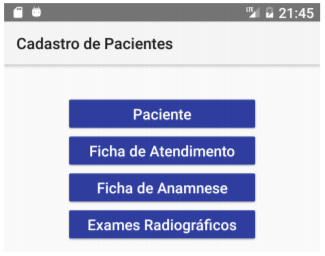
\includegraphics[scale=0.8]{cadastro-paciente}%% Dimensões e localização
\fonte{}%% Fonte
\end{figure}

\section{Implementação do sistema}\label{sec:implementacaoSistema}

Nesta seção é documentada a implementação do sistema com partes relevantes ou exemplos de código, rotinas, funções. Inclui, ainda, a descrição técnica do uso de recursos (componentes, bibliotecas, etc.) da linguagem. Ressalta-se que cada orientador avaliará juntamente com seu orientado o que poderá ser descrito nesta seção. Isso sem que sejam revelados detalhes do sistema que possam comprometer seu uso comercial ou científico ou que a descrição fique muito sucinta ou superficial.

Em materiais e método estão quais os recursos utilizados, neste capítulo é reportado como esses recursos foram utilizados para resolver o problema.

Sugere-se colocar listagens curtas de código, enfatizando aspectos específicos das tecnologias utilizadas ou da implementação. Sugere-se, ainda, que o código não seja apresentado sob a forma de print screen, e sim copiado e colado no texto, mantendo, se possível, a formatação. Todas as listagens de código devem ser devidamente explicadas. A explicação deve ser técnica, fundamentada em aspectos conceituais e boas práticas de programação.

Enfatizar os diferenciais do sistema: procedimentos armazenados, consultas SQL, uso de componentes, uso de padrões de projeto, a forma de uso dos recursos da linguagem. Esses diferenciais são no sentido de explicitar as vantagens, desvantagens, dificuldades e facilidades que esses recursos impetraram no desenvolvimento do sistema em termos técnicos. Esses diferenciais servirão para avaliar pela utilização ou não desses recursos, pelo menos para sistemas iguais ou semelhantes ao reportado no trabalho.

Reportar a forma como o sistema foi verificado e validado. No sentido de verificar se os requisitos definidos para o mesmo foram atendidos. Os testes podem ser realizados pelo professor orientador, pelos professores que compõem a banca, por pessoas que serviram de base para as informações para o sistema e etc. Os testes podem ser realizados com base em um plano de testes elaborado juntamente com a análise e projeto do sistema. Para validar a implementação podem ser desenvolvidas rotinas de teste unitário.

Se houver implantação do sistema, mesmo que seja para teste, reportar a forma como isso foi feito, a geração de instaladores, os problemas com ambiente e sistema operacional, incluindo banco de dados e outros. Deixar explícito o procedimento para instalar e usar o sistema.

Quando for necessário, citar no texto do trabalho nomes de campos, tabelas ou rotinas específicas utilizadas na implementação de um software, utilizar a fonte courier new para destacar esses nomes.

Um exemplo de listagem de código fonte pode ser observado na \autoref{codigo:classeFoo}, que representa a classe Aluno.

\begin{sourcecode}[htb]
\caption{\label{codigo:classeFoo}Classe Aluno}
\begin{lstlisting}[frame=single, language=Java]
@Entity
public class Foo {
 
    @Id
    @GeneratedValue(strategy = GenerationType.IDENTITY)
    private Long id;
 
    private String nome;
    
    private Integer ra;
     
    // constructor, getters and setters
}
\end{lstlisting}
\fonte{}
\end{sourcecode}

\section{Discussões (opcional)}\label{sec:discussoes} 

O trabalho contém esta seção quando considerado que há resultados (em termos de dados) e discussões relevantes ou suficientes para justificar uma seção. Se existentes e não justificarem uma seção, eles podem estar na seção que relata a implementação do sistema.

Nesta seção estão os resultados obtidos da realização de testes quantitativos e qualitativos, independentemente da quantidade, tipo e volume de testes realizados. Os resultados dos testes são discutidos tendo como base o referencial teórico e os objetivos pretendidos com o trabalho. Esses testes podem resultar de implantação e testes de uso do sistema. 
%% Comente para remover este item

%% Capítulo - esse capítulo contém exemplos para melhor uso do modelo Latex
%% Na versão final do TCC esse capítulo deve ser removido utilizando o sinal %
%%%%% CAPÍTULO - EXEMPLO
%%
%% Capítulo de informações e exemplos de utilização deste modelo.

%% Título e rótulo de capítulo (rótulos não devem conter caracteres especiais, acentuados ou cedilha)
\chapter{Informações e Exemplos de Utilização deste Modelo}\label{cap:exemplo}

Devido à necessidade de padronização em trabalhos acadêmicos (teses, dissertações, trabalhos de conclusão de curso, etc.), são utilizadas neste documento algumas regras básicas para estruturação e formatação.

O presente documento/\textit{template} foi produzido em parceria entre a \gls{utfpr} de Pato Branco e a \gls{utfpr} de Campo Mourão. Assim, derivado do \gls{utfprpbtex}\index{UTFPRPBTeX@\utfprpbtex} e de alterações implementadas pela UTFPR de Campo Mourão, surge o \utfprtex, como um proposta de um modelo \latex que pode ser utilizado por qualquer campus da \gls{utfpr} para elaboração de trabalhos acadêmicos segundo as normas definidas pela \gls{abnt}\index{ABNT}. Este modelo foi desenvolvido em linguagem de editoração \gls{tex}\index{TeX@\TeX}/\gls{latex}\index{LaTeX@\latex} com base no modelo \gls{abntex2}\index{abnTeX2@\abnTeX} \cite{abnTeX2:2013}, que atende os requisitos das normas da ABNT para elaboração de documentos técnicos e científicos brasileiros.

Os principais arquivos do modelo são: 
\begin{itemize}
    \item \texttt{main.tex} - é o arquivo principal que relaciona todos os outros arquivos, neste você pode remover ou adicionar elementos textuais (capítulos, etc);
    \item \texttt{configuracoes.tex} - contém os pacotes a serem utilizados pelo ambiente, bem como a criação de comandos do \latex;
    \item \texttt{variaveis.tex} - contém variáveis, como nome do autor, orientador, título, banca e que devem ser alterados para atender cada trabalho;
    \item \texttt{main.bib} - contém as referências bibliográficas;
    \item \texttt{readme.md} - são informações a respeito do template \latex;
    \item \texttt{utfpr.cls} - mantém a formatação do texto - \textbf{não altere esse arquivo a menos que você saiba o que está fazendo}.
\end{itemize}

Além dos arquivos, o \textit{template} contém diretórios/pastas, para ajudar a organizar o trabalho, sendo essas:
\begin{itemize}%% Lista de itens
\item \texttt{PreTexto} - contém arquivos, com nomes auto descritivos, que representam elementos pré textuais como:  resumo, abstract, agradecimentos, siglas, epigrafe, etc;
\item \texttt{capitulos} -  contém arquivos, com nomes auto descritivos, que representam os capítulos do texto, como por exemplo: introdução, metodologia, conclusão, etc. Para adicionar ou remover um capítulo é necessário alterar o arquivo \texttt{main.tex} - ver exemplos no próprio arquivo;
\item \texttt{figuras}  - contém as figuras/imagens utilizadas no texto;
\item \texttt{PosTexto} - contém elementos pós textuais como: anexo, apêndice, etc.
\end{itemize}

A codificação de caracteres em todos os arquivos é \texttt{UTF8}, tanto no modelo \gls{abntex2}\index{abnTeX2@\abnTeX} quanto no modelo \gls{utfprpbtex}\index{UTFPRPBTeX@\utfprtex}. Portanto, é necessário que seja utilizada a mesma codificação nos documentos a serem desenvolvidos, inclusive nos arquivos de base bibliográfica. Diversos editores de arquivos fonte do \gls{latex}\index{LaTeX@\latex} são capazes de manipular e/ou converter entre diferentes codificações, por exemplo, o ``Texmaker\index{Texmaker}'' (disponível em \url{http://www.xm1math.net/texmaker/}). 
%Recomenda-se, sempre que for manipular e/ou substituir um dos arquivos constituintes deste modelo, manter uma cópia do original num local seguro e/ou renomear esta cópia do original para que possa ser utilizada como um exemplo no desenvolvimento do seu próprio arquivo. Por exemplo, quando for criar o seu ``Capítulo 1'', fazer uma cópia do arquivo original \texttt{capitulo1.tex}, renomeando-o para \texttt{capitulo1.original.tex}, por exemplo, e realizar as alterações e/ou modificações no arquivo \texttt{capitulo1.tex}.

Este capítulo\label{errata:capitulo} de exemplo tem por finalidade a definição e a apresentação de alguns comandos do \gls{latex}\index{LaTeX@\latex} e/ou dos modelos \gls{abntex2}\index{abnTeX2@\abnTeX} e \gls{utfprpbtex}\index{UTFPRPBTeX@\utfprtex}. O presente documento não se constitui um manual, tampouco uma apostila de \gls{latex}\index{LaTeX@\latex}, visto que existe uma grande quantidade de material de referência disponível na Internet, como por exemplo em \url{http://en.wikibooks.org/wiki/LaTeX}.

Os capítulos devem conter uma introdução e um fecho. A introdução fornece ao leitor uma breve descrição do que será tratado no capítulo, enquanto o fecho apresenta comentários finais sobre o que foi desenvolvido no capítulo. Os capítulos podem ser divididos em seções\label{errata:secao}. Esta divisão deve ser lógica (temática) e não física (por tamanho). O número ideal de seções é impossível de se precisar. Entretanto, um capítulo com uma única seção, possivelmente, deverá ser agregado ao capítulo anterior ou posterior. Um capítulo com quinze seções, possivelmente, deverá ser subdividido em dois capítulos. Capítulos, seções e subseções\label{errata:subsecao} devem ser rotulados para que possam ser referenciados em qualquer parte do texto. Exemplo: O \autoref{cap:exemplo} é gerado, rotulado e referenciado pelos comandos \verb|\chapter{Informações e...}|, \verb|\label{cap:exemplo}| e \verb|\autoref{cap:exemplo}|, respectivamente.

%% Título e rótulo de seção (rótulos não devem conter caracteres especiais, acentuados ou cedilha)
\section{Título da seção secundária}\label{sec:secsec}

Seções secundárias são divisões do conteúdo das seções primárias. A \autoref{sec:secsec} é gerada, rotulada e referenciada pelos comandos \verb|\section{Título da Seção Secundária}|, \verb|\label{sec:secsec}| e \verb|\autoref{sec:secsec}|, respectivamente.

%% Título e rótulo de seção (rótulos não devem conter caracteres especiais, acentuados ou cedilha)
\subsection{Título da seção terciária}\label{ssec:secterc}

Seções terciárias são divisões do conteúdo de seções secundárias. A \autoref{ssec:secterc} é gerada, rotulada e referenciada pelos comandos \verb|\subsection{Título da Seção Terciária}|, \verb|\label{ssec:secterc}| e \verb|\autoref{ssec:secterc}|, respectivamente.

%% Título e rótulo de seção (rótulos não devem conter caracteres especiais, acentuados ou cedilha)
\subsubsection{Título da seção quartenária}\label{sssec:secquart}

Seções quartenárias são divisões do conteúdo de seções terciárias. A \autoref{sssec:secquart} é gerada, rotulada e referenciada pelos comandos \verb|\subsubsection{Título da seção quartenária}|, \verb|\label{sssec:secquart}| e \verb|\autoref{sssec:secquart}|, respectivamente.

%% Título e rótulo de seção (rótulos não devem conter caracteres especiais, acentuados ou cedilha)
\section{Exemplo de título de seção secundária com um texto muito longo que pode ocupar mais de uma linha}\label{sec:sectitulolongo}

A \autoref{sec:sectitulolongo} é um exemplo de título de seção secundária com texto muito longo, formatado automaticamente de acordo com \citeonline[subseções 5.2.2 a 5.2.4]{NBR14724:2011} e \citeonline[subseções 3.1 a 3.8]{NBR6024:2012}. Segundo as normas, o título de seção deve estar alinhado à esquerda e a segunda e demais linhas devem iniciar logo abaixo da primeira palavra da primeira linha.

%% Título e rótulo de seção (rótulos não devem conter caracteres especiais, acentuados ou cedilha)
\section{Elementos pré-textuais}\label{sec:elempretext}

Alguns elementos pré-textuais do presente documento são gerados automaticamente pelo \gls{utfprpbtex}\index{UTFPRPBTeX@\utfprtex}. Para adicionar e/ou alterar as informações apresentadas na capa, na folha de rosto %, na ficha catalográfica 
e na folha de aprovação deve-se editar o arquivo \texttt{variaveis.tex}. %Os dados informados neste arquivo também são utilizados para gerar a referência do trabalho na errata, no resumo e no \textit{abstract}.

Para adicionar e/ou alterar o texto da errata, da dedicatória, dos agradecimentos, da epígrafe, do resumo e do \textit{abstract} deve-se editar seus respectivos arquivos presentes no diretório ``PreTexto'': \texttt{errata.tex}, \texttt{dedicatoria.tex}, \texttt{agradecimentos.tex}, \texttt{epigrafe.tex}, \texttt{resumo.tex} e \texttt{abstract.tex}.

As listas de algoritmos, de ilustrações e de tabelas são geradas automaticamente pelo \gls{utfprpbtex}\index{UTFPRPBTeX@\utfprtex}. Os itens destas listas são gerados a medida que forem sendo inseridos no texto do documento. 

A lista de abreviaturas, siglas e acrônimos pode ser gerada automaticamente por meio do arquivo \texttt{entradas-acronimos.tex}, utilizando o pacote \texttt{glossaries}\footnote{Detalhes sobre comandos para geração de abreviaturas, siglas e acrônimos utilizando o pacote \texttt{glossaries} são apresentadas na \autoref{sec:acronimos}.}, ou por meio da edição do arquivo \texttt{lista-acronimos.tex}. A lista de símbolos pode ser gerada automaticamente utilizando o pacote \texttt{nomencl}\footnote{Detalhes sobre comandos para geração de símbolos utilizando o pacote \texttt{nomencl} são apresentadas na \autoref{sec:simbolos}.} ou mediante a edição do arquivo \texttt{lista-simbolos.tex}. Os arquivos citados estão no diretório ``PreTexto''. O sumário é o último elemento pré-textual e também é gerado automaticamente pelo \gls{utfprpbtex}\index{UTFPRPBTeX@\utfprtex}.

%% Título e rótulo de seção (rótulos não devem conter caracteres especiais, acentuados ou cedilha)
\section{Regras gerais de apresentação}\label{sec:regrasgerais}

As regras gerais de apresentação, definidas na sequência, já estão predefinidas no modelo \gls{utfprpbtex}\index{UTFPRPBTeX@\utfprtex}. Algumas destas regras podem ser alteradas, por comandos apropriados do \gls{latex}\index{LaTeX@\latex}, do \gls{abntex2}\index{abnTeX2@\abnTeX} ou do \gls{utfprpbtex}\index{UTFPRPBTeX@\utfprtex}, no preâmbulo do arquivo principal \texttt{configuracoes.tex} ou em outras partes do documento, por exemplo, nos capítulos.

\begin{itemize}%% Lista de itens
\item Configuração das margens: deve-se usar margens superior e esquerda de \SI{3}{cm}; e margens inferior e direita de \SI{2}{cm}; em papel formato A4 ($\SI{21}{cm} \times \SI{29,7}{cm}$);
\item Recomenda-se o uso de fonte tipo Arial ou Times New Roman, tamanho 12 para o texto e tamanho 10 para citações de mais de três linhas, notas de rodapé e legendas dos algoritmos, ilustrações e tabelas;
\item O parágrafo deve aparecer com recuo na primeira linha de \SI{1,5}{cm}, justificado, sem espaçamento anterior ou posterior;
%\item Os elementos como: o resumo, as notas, as referências, as legendas das ilustrações e tabelas, a natureza do trabalho, o objetivo, o nome da instituição a que é submetida e a área de concentração devem ser digitados em espaço simples.
\item A numeração progressiva para as seções do texto deve ser adotada para evidenciar a sistematização do conteúdo do trabalho;
\item Para os títulos das seções não se utilizam pontos, hífen, travessão, ou qualquer sinal após o indicativo de seção ou de título;
\item Para as seções primárias: utiliza-se negrito e caixa alta;
\item Para as seções secundárias: título em negrito, iniciado em letra maiúscula e demais letras minúsculas;
\item Para as seções terciárias: somente a primeira letra do título da seção em
maiúscula;
\item Para as seções quaternárias: título da seção sublinhado, com inicial em letra maiúscula e demais letras minúsculas.
\item No sumário, os títulos das seções devem aparecer exatamente iguais ao que estão contidos no trabalho.
\end{itemize}

\caixa{Atenção}{No \latex é necessário manter os títulos apenas com a primeira letra maiúscula e o restante em minúsculo, o retante é controlado pelo \latex, então não é necessário se preocupar com a formatação!}

Recomenda-se evitar, sempre que possível, o uso dos seguintes recursos (ou enfeites) no documento:

\begin{itemize}%% Lista de itens
\item \textbf{o uso de negrito;}
\item \textit{o uso de itálico (exceto em palavras em outra língua);}
\item \texttt{texto em diferente fonte como máquina de escrever;}
\item \underline{o uso de texto sublinhado;}
\item o uso excessivo de\footnote{Notas de rodapé.}.
\end{itemize}

\noindent Lembre-se: um texto ``limpo'' é mais agradável de ler que um texto ``enfeitado''.

%% Título e rótulo de seção (rótulos não devem conter caracteres especiais, acentuados ou cedilha)
\subsection{Espaçamento}\label{sec:espacamento}

\begin{itemize}%% Lista de itens
%\item O resumo, o \textit{abstract}, as notas, as referências, as legendas das ilustrações e tabelas e a natureza do trabalho devem ser digitadas em espaço simples.
\item Todo o texto deve ser formatado com espaço entre linhas de um fator de 1,5 (sem espaçamento antes/depois).
\item As citações com mais de três linhas devem ser em espaço simples e com recuo de \SI{4}{cm} da margem esquerda.
\item As referências, ao final do trabalho, devem ser separadas entre si por um espaços simples, e na mesma referência o espaço é simples.
%\item Os títulos das seções secundárias devem ser separados do texto que os precede por dois espaços entre linhas de um fator de 1,5.
\item As seções primárias devem iniciar em páginas distintas.
\end{itemize}

O recuo na primeira linha, espaço entre a margem e o início do parágrafo, pode ser redefinido definido pelo comando:

\begin{SingleSpacing}%% Ambiente SingleSpacing
\begin{verbatim}
\setlength{\parindent}{1.5cm}
\end{verbatim}
\end{SingleSpacing}

O espaçamento entre um parágrafo e outro\index{espaçamento!entre os parágrafos} pode ser redefinido pelo comando:

\begin{SingleSpacing}%% Ambiente SingleSpacing
\begin{verbatim}
\setlength{\parskip}{0mm} %% Tente também \onelineskip
\end{verbatim}
\end{SingleSpacing}

O controle do espaçamento entre linhas\index{espaçamento!entre as linhas} pode ser redefinido pelo comando:

\begin{SingleSpacing}%% Ambiente SingleSpacing
\begin{verbatim}
\OnehalfSpacing %% Espaçamento um e meio (padrão)
\DoubleSpacing  %% Espaçamento duplo
\SingleSpacing  %% Espaçamento simples
\end{verbatim}
\end{SingleSpacing}

Para isso, também estão disponíveis os ambientes:

\begin{SingleSpacing}%% Ambiente SingleSpacing
\begin{verbatim}
\begin{SingleSpacing} ...     \end{SingleSpacing}
\begin{Spacing}{<factor>} ... \end{Spacing}
\begin{OnehalfSpacing} ...    \end{OnehalfSpacing}
\begin{OnehalfSpacing*} ...   \end{OnehalfSpacing*}
\begin{DoubleSpacing} ...     \end{DoubleSpacing}
\begin{DoubleSpacing*} ...    \end{DoubleSpacing*}
\end{verbatim}
\end{SingleSpacing}

Para mais informações, consulte \citeonline[p. 47-52 e 135]{Wilson2010}.

\subsection{Exemplo de quantidades de subseções}\label{sec:exSubsec}

Quando um item é dividido, precisa ter pelo menos dois sub-itens (não pode ter apenas um), por exemplo para ter a subseção 4.1 é obrigatório ter pelo menos a subseção 4.2, não pode somente a primeira subseção.

%% Título e rótulo de seção (rótulos não devem conter caracteres especiais, acentuados ou cedilha)
\section{Enumerações: alíneas e subalíneas}\label{sec:enumeracoes}\index{alíneas}\index{subalíneas}

Quando for necessário enumerar os diversos assuntos de uma seção que não possua título, esta deve ser subdividida em alíneas\index{alíneas} \cite[subseção 4.2]{NBR6024:2012}:

\begin{alineas}%% Ambiente alineas
\item os diversos assuntos que não possuam título próprio, dentro de uma mesma seção, devem ser subdivididos em alíneas\index{alíneas};
\item o texto que antecede as alíneas\index{alíneas} termina em dois pontos;
\item as alíneas\index{alíneas} devem ser indicadas alfabeticamente, em letra minúscula, seguida de parêntese. Utilizam-se letras dobradas, quando esgotadas as letras do alfabeto;
\item as letras indicativas das alíneas\index{alíneas} devem apresentar recuo em relação à margem esquerda;
\item o texto da alínea deve começar por letra minúscula e terminar em ponto-e-vírgula, exceto a última alínea que termina em ponto final;
\item o texto da alínea deve terminar em dois pontos, se houver subalínea;
\item a segunda e as seguintes linhas do texto da alínea começa sob a primeira letra do texto da própria alínea;
\item subalíneas\index{subalíneas} \cite[subseção 4.3]{NBR6024:2012} devem ser conforme as alíneas\index{alíneas} a seguir:
\begin{alineas}%% Ambiente alineas
\item as subalíneas\index{subalíneas} devem começar por travessão seguido de espaço;
\item as subalíneas\index{subalíneas} devem apresentar recuo em relação à alínea;
\item o texto da subalínea deve começar por letra minúscula e terminar em ponto-e-vírgula. A última subalínea deve terminar em ponto final, se não houver alínea subsequente;
\item a segunda e as seguintes linhas do texto da subalínea começam sob a primeira letra do texto da própria subalínea.
\end{alineas}
\item no \gls{abntex2}\index{abnTeX2@\abnTeX} estão disponíveis os ambientes \texttt{incisos} e \texttt{subalineas}, que em suma são o mesmo que se criar outro nível de \texttt{alineas}, como nos exemplos à seguir:
\begin{incisos}%% Ambiente incisos
\item \textit{um novo inciso em itálico}\index{incisos}.
\end{incisos}
\item Alínea em \textbf{negrito}:
\begin{subalineas}%% Ambiente subalineas
\item \textit{uma subalínea em itálico};
\item \underline{\textit{uma subalínea em itálico e sublinhado}}.
\end{subalineas}
\item última alínea com \emph{ênfase}.
\end{alineas}

%% Título e rótulo de seção (rótulos não devem conter caracteres especiais, acentuados ou cedilha)
\section{Citações}\label{sec:citacoes}

O \gls{utfprpbtex}\index{UTFPRPBTeX@\utfprtex} está configurado para produzir as citações no texto no estilo alfabético (autor-data), segundo as normas \gls{abnt}\index{ABNT}, por meio dos comandos do \gls{abntex2}\index{abnTeX2@\abnTeX} \cite{abnTeX2:2013Cite,abnTeX2:2013CiteAlf}. A lista dos principais comandos são apresentadas a seguir:

\begin{itemize}%% Lista de itens
\item \verb|\cite{rótulo}| -- para gerar citação implícita. Por exemplo, a citação ``\ldots\ \cite{Thompson2001}\ldots'' é gerada pelo comando \verb|\cite{Thompson2001}| ou pelo atalho \verb|\citep{Thompson2001}|, definido em \texttt{utfprpb.tex}.
\item \verb|\citeonline{rótulo}| -- para gerar citação explícita. Por exemplo a citação ``\ldots\ conforme proposto por \citeonline{Thompson2001}\ldots'' é gerada pelo comando \verb|\citeonline{Thompson2001}| ou pelo atalho \verb|\citet{Thompson2001}|, definido em \texttt{utfprpb.tex}.
\item \verb|(\citeauthor{rótulo})| -- para gerar citação implícita somente do autor. Por exemplo, a citação ``\ldots\ (\citeauthor{Thompson2001})\ldots'' é gerada pelo comando \verb|(\citeauthor{Thompson2001})| ou pelo atalho \verb|\citepa{Thompson2001}|, definido em \texttt{utfprpb.tex}.
\item \verb|\citeauthoronline{rótulo}| -- para gerar citação explícita somente do autor. Por exemplo, a citação ``\ldots\ conforme a relação de \citeauthoronline{Thompson2001}\ldots'' é gerada pelo comando \verb|\citeauthoronline{Thompson2001}| ou pelo atalho \verb|\citeta{Thompson2001}|, definido em \texttt{utfprpb.tex}.
\item \verb|(\citeyear{rótulo})| -- para gerar citação implícita somente do ano. Por exemplo, a citação ``\ldots\ (\citeyear{Thompson2001})\ldots'' é gerada pelo comando \verb|(\citeyear{Thompson2001})| ou pelo atalho \verb|\citepy{Thompson2001}|, definido em \texttt{utfprpb.tex}.
\item \verb|\citeyear{rótulo}| -- para gerar citação explícita somente do ano. Por exemplo, a citação ``\ldots\ no ano de \citeyear{Thompson2001}\ldots'' é gerada pelo comando \verb|\citeyear{Thompson2001}| ou pelo atalho \verb|\citety{Thompson2001}|, definido em \texttt{utfprpb.tex}.
\end{itemize}

Informações sobre a utilização dos comandos listados acima e os demais comandos para geração de referências, utilizados pelo \gls{abntex2}\index{abnTeX2@\abnTeX}, podem ser encontradas em \citeonline{abnTeX2:2013Cite,abnTeX2:2013CiteAlf}, disponíveis em \url{http://www.abntex.net.br/}.

\gls{latex}\index{LaTeX@\latex} utiliza um arquivo externo (em separado) para o banco de dados das referências citadas no texto. Este arquivo é compilado pelo \gls{bibtex}\index{BibTeX@Bib\TeX} e deve possuir a extensão \texttt{bib}, como nos arquivos \texttt{referencias.bib} e \texttt{referencias-modelos.bib} presentes no diretório ``PosTexto'', utilizados neste documento. O arquivo \texttt{referencias-modelos.bib} apresenta exemplos dos seguintes estilos de referência aceitos pelo \gls{bibtex}\index{BibTeX@Bib\TeX}:

\begin{itemize}%% Lista de itens
\item anais de simpósios \citep{Alt1995,Pirmez2002};
\item artigos em anais de simpósios \citep{Faina2001};
\item artigos em coletâneas de artigos \citep{Pinto2000};
\item artigos em revistas \citep{Guimaraes2003};
\item capítulos de livros \citep{Santos2000};
\item livretos \citep{Thompson2001};
\item livros \citep{Pedrycz1998};
\item manuais técnicos \citep{IONA1999};
\item miscelânea \citep{Cruz2003};
\item páginas na Internet \cite[acessado em 1 de janeiro de 2004]{Larsson2003} (utilizar a data do último acesso à página);
\item relatórios técnicos \citep{OMG2000};
\item teses de mestrado \citep{SantosFilho2003};
\item teses de doutorado \citep{Faina2000};
\item trabalhos não publicados \citep{Sichman2002}.
\end{itemize}

\subsection{Programas úteis para citações}\label{sec:progUteisCitacoes}

Existem alguns programas para gerenciamento de banco de dados de referências bibliográficas (arquivos \texttt{bib}) do \gls{bibtex}\index{BibTeX@Bib\TeX}. O ``JabRef'' é um exemplo destes programas e está disponível em: \url{http://jabref.sourceforge.net/}.

%% Título e rótulo de seção (rótulos não devem conter caracteres especiais, acentuados ou cedilha)
\subsection{Citações diretas}\label{sec:citacoesdiretas}\index{citações!diretas}

O ambiente \texttt{citacao} permite a inclusão de citações diretas que ocupam mais de três linhas:

\begin{citacao}%% Ambiente citacao
As citações diretas no texto, que ocupam mais de três linhas, devem ser destacadas com recuo de \SI{4}{cm} da margem esquerda, com letra menor que a do texto utilizado e sem as aspas. No caso de documentos datilografados, deve-se observar apenas o recuo \cite[subseção 5.3]{NBR10520:2002}.
\end{citacao}

\noindent Esta citação direta com mais de três linhas foi gerada da seguinte forma:

\begin{SingleSpacing}%% Ambiente SingleSpacing
\begin{verbatim}
\begin{citacao}
As citações diretas no texto, com mais de três linhas,...
... observar apenas o recuo \cite[subseção 5.3]{NBR10520:2002}.
\end{citacao}
\end{verbatim}
\end{SingleSpacing}

O ambiente \texttt{citacao} pode receber como parâmetro opcional um nome de idioma previamente carregado nas opções da classe (definido no preâmbulo do arquivo \texttt{utfprpb.tex}). Neste caso, o texto da citação é automaticamente escrito em itálico e a hifenização é ajustada para o idioma selecionado na opção do ambiente. Por exemplo:

\begin{SingleSpacing}%% Ambiente SingleSpacing
\begin{verbatim}
\begin{citacao}[english]
Text in English language in italic with correct hyphenation.
\end{citacao}
\end{verbatim}
\end{SingleSpacing}

\noindent Tem como resultado:

\begin{citacao}[english]%% Ambiente citacao
Text in English language in italic with correct hyphenation.
\end{citacao}

Citações simples\index{citações!simples}, com até três linhas, devem ser incluídas com aspas. Observe que em \gls{latex}\index{LaTeX@\latex} as aspas iniciais são diferentes das finais: ``Amor é fogo que arde sem se ver''.

%% Título e rótulo de seção (rótulos não devem conter caracteres especiais, acentuados ou cedilha)
\section{Equações}\label{sec:equacoes}

\gls{latex}\index{LaTeX@\latex} é insuperável no processamento de equações. Equações simples como $y = a x^2 + b x + c$ podem ser adicionadas ao longo do texto ou em uma linha própria:
%
\[%% Ambiente displaymath
y = a x^2 + b x + c
\]

Equações complexas como:
%
\begin{equation}%% Ambiente equation
\label{eq:equation1}%% Rótulo
\begin{array}{lcl}%% Ambiente array
p \left(\gamma\right)
& = &
\frac{1}{2}
\sqrt{\frac{M}{\gamma \bar{\gamma}_b}}
\frac{1}{\prod_{i = 1}^M \sqrt{\tilde{\gamma}_i}}
\int_0^{\sqrt{M \delta}}
\int_0^{\sqrt{M \delta} - r_M} \cdots
\int_0^{\sqrt{M \delta} - \sum_{i = 3}^M r_i} \\[0.5\linha]
& &
p \left(%
\frac{\sqrt{M \delta} - \sum_{i = 2}^M r_i}{\sqrt{\tilde{\gamma}_1}},
\frac{r_2}{\sqrt{\tilde{\gamma}_2}}, \ldots,
\frac{r_M}{\sqrt{\tilde{\gamma}_M}}
\right) \, \der r_2 \cdots \der r_{M - 1} \, \der r_M
\end{array}
\end{equation}

\noindent ou
%
\begin{equation}%% Ambiente equation
\label{eq:equation2}%% Rótulo
T \left(r\right) =
\frac{1}{f_m}
\left(%
\frac{\pi}{2} \sum_{i = 1}^M {\tilde{r}_i^2 \dot{\varsigma}_i^2}
\right)^{-1/2}
\frac{%
\begin{array}{ll}%% Ambiente array
\int_0^{\rho \sqrt{M}}
\int_0^{\rho \sqrt{M} - r_M} \cdots
\int_0^{\rho \sqrt{M} - \sum_{i = 3}^M r_i}
\int_0^{\rho \sqrt{M} - \sum_{i = 2}^M r_i} \\[0.5\linha]
p \left(%
\frac{r_1}{\tilde{r}_1},
\frac{r_2}{\tilde{r}_2}, \ldots,
\frac{r_M}{\tilde{r}_M}
\right) \, \der r_1 \, \der r_2 \cdots \der r_{M - 1} \, \der r_M \\[0.5\linha]
\end{array}
}{%
\begin{array}{ll}%% Ambiente array
\int_0^{\rho \sqrt{M}}
\int_0^{\rho \sqrt{M} - r_M} \cdots
\int_0^{\rho \sqrt{M} - \sum_{i = 3}^M r_i} \\[0.5\linha]
p \left(%
\frac{\rho \sqrt{M} - \sum_{i = 2}^M r_i}{\tilde{r}_1},
\frac{r_2}{\tilde{r}_2}, \ldots,
\frac{r_M}{\tilde{r}_M}
\right) \, \der r_2 \cdots \der r_{M - 1} \, \der r_M \\[0.5\linha]
\end{array}
}
\end{equation}

\noindent são automaticamente numeradas e podem ser referenciadas ao longo do texto. Por exemplo, a \seqref{eq:equation1} é trivialmente derivada da \seqref{eq:equation2}. Veja os exemplos de comandos para estas equações no arquivo fonte deste capítulo.

%% Título e rótulo de seção (rótulos não devem conter caracteres especiais, acentuados ou cedilha)
\section{Algoritmos}\label{sec:algoritmos}

Algoritmos podem ser inseridos por meio do pacote \texttt{algorithms}, conforme exemplos no arquivo fonte deste capítulo e cujos resultados são apresentados no \autoref{alg:algoritmo1} e no \autoref{alg:algoritmo2}.

\begin{algorithm}[htb]%% Ambiente algorithm
\caption{Primeiro exemplo de algoritmo com uma legenda contendo um texto muito longo que pode ocupar mais de uma linha}%% Legenda
\label{alg:algoritmo1}%% Rótulo
\hrule
\begin{algorithmic}[1]%% Ambiente algorithmic
\ENSURE $A, B$
\STATE $C = A + B$
\PRINT $C$
\end{algorithmic}
\hrule
\fonte{}%% Fonte
\end{algorithm}

\begin{algorithm}[htb]%% Ambiente algorithm
\caption{Segundo exemplo de algoritmo}%% Legenda
\label{alg:algoritmo2}%% Rótulo
\hrule
\begin{algorithmic}[1]%% Ambiente algorithmic
\ENSURE $A, B$
\STATE $C = A + B$
\IF{$C < 10$}
\STATE $C = 2 \ C$
\ELSE
\STATE $C = 0,5 \ C$
\ENDIF
\PRINT $A, B, C$
\end{algorithmic}
\hrule
\fonte{}%% Fonte
\end{algorithm}

A documentação sobre o pacote \texttt{algorithms} pode ser encontrada em: \url{http://tug.ctan.org/tex-archive/macros/latex/contrib/algorithms/algorithms.pdf}.

%% Título e rótulo de seção (rótulos não devem conter caracteres especiais, acentuados ou cedilha)
\section{Ilustrações}\label{sec:ilustracoes}

O \gls{utfprpbtex}\index{UTFPRPBTeX@\utfprtex} está configurado para produzir os ambientes para os seguintes tipos de ilustrações: figuras, fotografias, gráficos e quadros. Exemplos de uso destes ambientes podem ser observados no arquivo fonte deste capítulo.

%% Título e rótulo de seção (rótulos não devem conter caracteres especiais, acentuados ou cedilha)
\subsection{Figuras}\label{sec:figuras}

Figuras são criadas e/ou editadas com editores gráficos capazes de exportar a figura em formato \gls{ps} ou, preferencialmente, \gls{eps}. O editor ``xfig'' é adequado para a maioria dos casos, como por exemplo, a \autoref{fig:figura1} que foi editada utilizando o ``xfig''. Outras opções para criação/edição de figuras são o GIMP (\url{http://www.gimp.org/}), ou o ``dia'' (\url{http://dia-installer.de/}), um editor orientado a diagramas (UML, fluxograma, etc.) com capacidade de exportar \gls{eps}, como apresentado por \citet{Larsson2003}.

%\gls{gimp}\index{Gimp}
\begin{figure}[htb]%% Ambiente figure
%\captionsetup{width=0.55\textwidth}%% Largura da legenda
\caption{Exemplo de figura criada a partir de um arquivo}%% Legenda
\label{fig:figura1}%% Rótulo
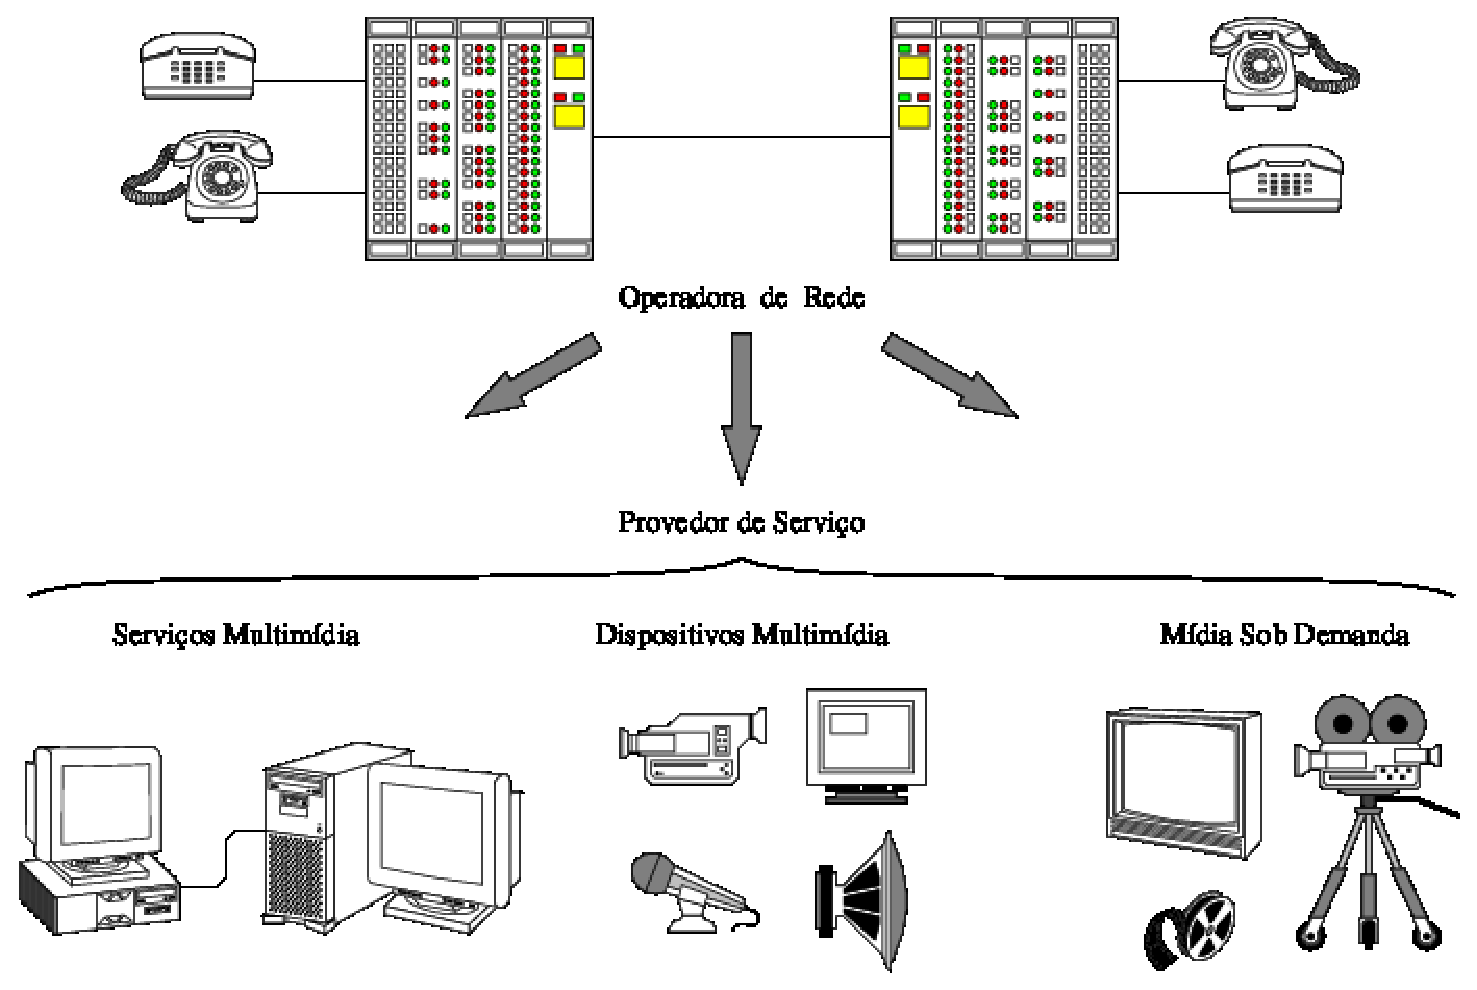
\includegraphics[width=0.6\textwidth]{figura1}%% Dimensões e localização
\fonte{\citet{Larsson2003}}%% Fonte
\end{figure}

Figuras em formato GIF, JPEG e BMP podem ser convertidas para o formato \gls{eps} por meio do aplicativo ``xv''. O ``xv'' não lista o formato \gls{eps} dentre aqueles que é capaz de manipular. Entretanto, selecionando-se o formato \textit{PostScript} e fornecendo-se a extensão \texttt{eps} ao nome do arquivo, o formato \gls{eps} é gerado.

O ambiente \texttt{picture} permite a programação de imagens diretamente no \gls{latex}\index{LaTeX@\latex}, conforme exemplo apresentado na \autoref{fig:figura2}.

\begin{figure}[htb]%% Ambiente figure
%\captionsetup{width=8cm}%% Largura da legenda
\caption{Exemplo de figura criada a partir do ambiente \texttt{picture}}%% Legenda
\label{fig:figura2}%% Rótulo
\setlength{\unitlength}{1cm}%% Unidade de comprimento
\begin{picture}(8,5)(-4,-2.5)%% Ambiente picture
\put(-4,0){\vector(1,0){8}}
\put(3.75,-0.25){$\chi$}
\put(0,-2.5){\vector(0,1){5}}
\multiput(-4,1)(0.4,0){20}{\line(1,0){0.2}}
\multiput(-4,-1)(0.4,0){20}{\line(1,0){0.2}}
\put(0.25,2.25){$\beta \equiv v / c = \tanh \chi$}
\qbezier(0,0)(0.8853,0.8853)(2,0.9640)
\qbezier(0,0)(-0.8853,-0.8853)(-2,-0.9640)
\end{picture}
\fonte{}%% Fonte
\end{figure}

%% Título e rótulo de seção (rótulos não devem conter caracteres especiais, acentuados ou cedilha)
\subsection{Fotografias}\label{sec:fotografias}

Um exemplo deste tipo de ilustração é apresentado na \autoref{foto:foto1}.

\begin{photograph}[htb]%% Ambiente photograph
%\captionsetup{width=0.6\textwidth}%% Largura da legenda
\caption{Camaleão pantera fotografado por Joel Sartore, National Geographic}%% Legenda
\label{foto:foto1}%% Rótulo
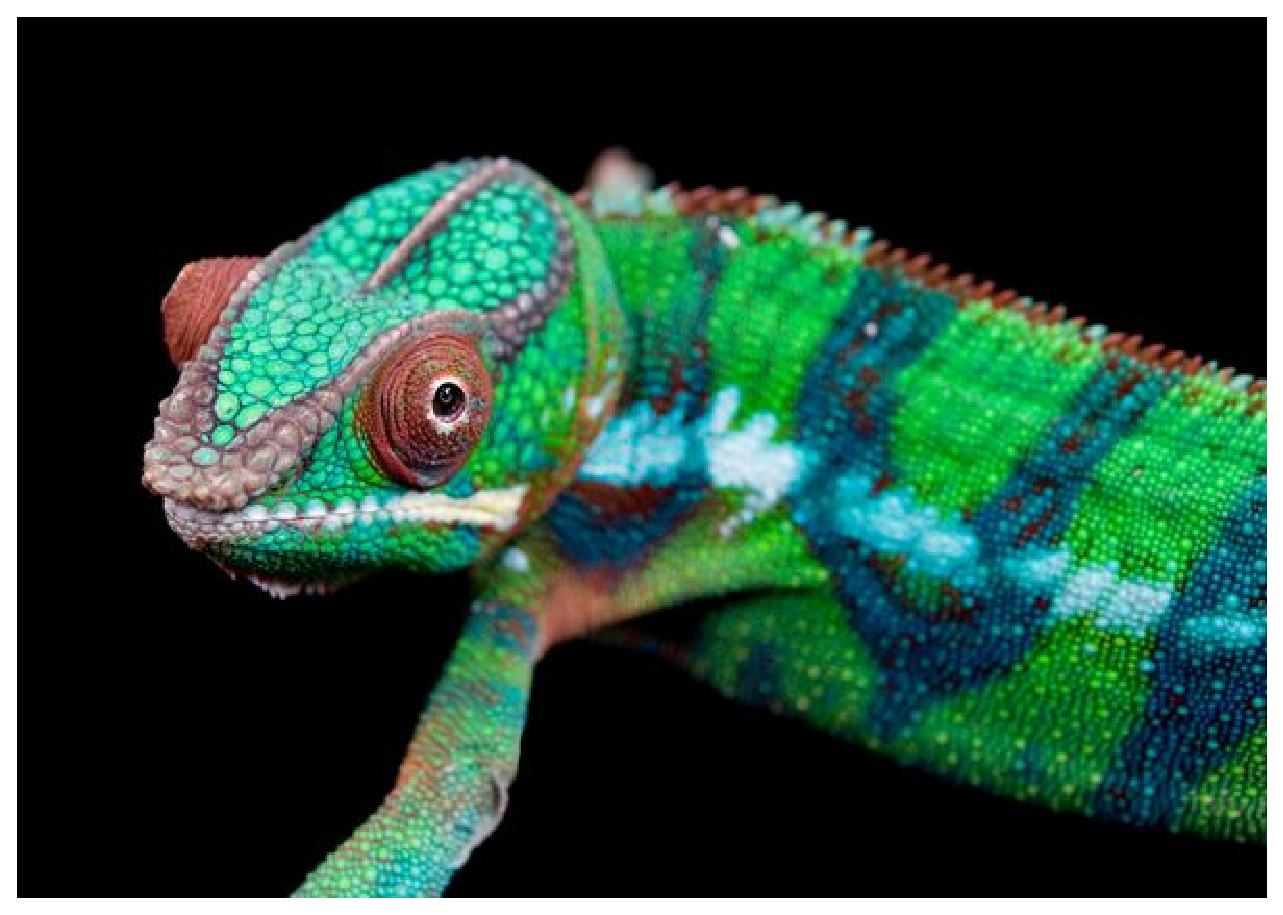
\includegraphics[width=0.95\textwidth]{foto1}%% Dimensões e localização
\fonte{\citet{Sartore2013}}%% Fonte
\end{photograph}

Outro exemplo deste tipo de ilustração é apresentado na \autoref{foto:foto2}.

\begin{photograph}[htb]%% Ambiente photograph
\captionsetup{width=0.6\textwidth}%% Largura da legenda
\caption{Fotografia da erupção vulcânica em 1982 do Galungung, Indonésia (com descargas de raios), produzida pelo Serviço Geológico dos Estados Unidos da América}%% Legenda
\label{foto:foto2}%% Rótulo
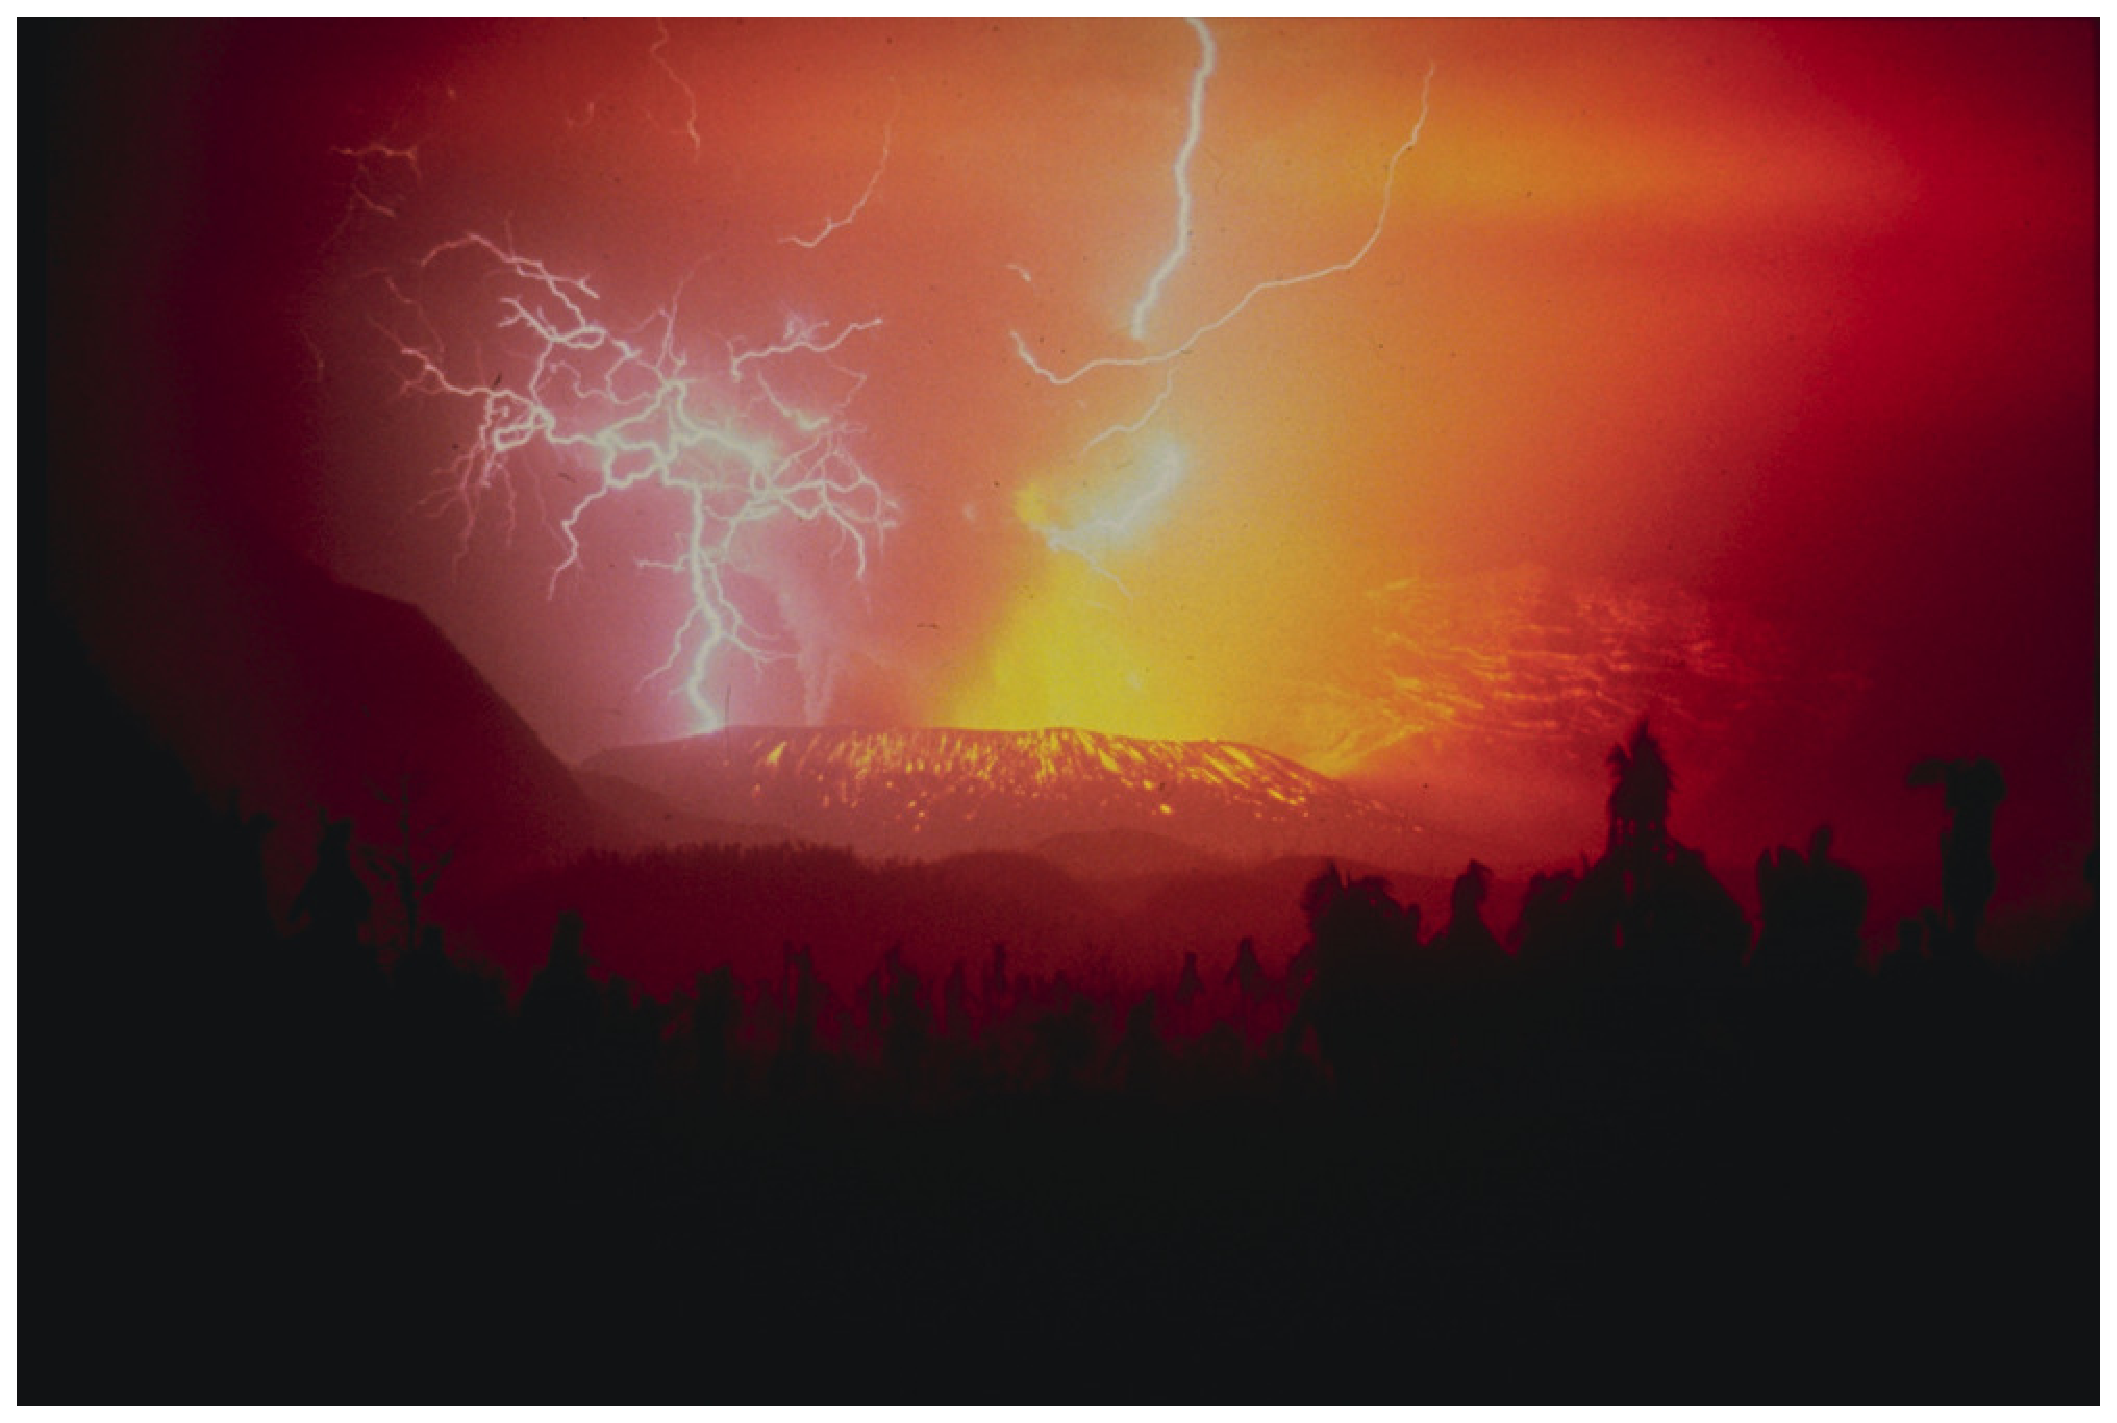
\includegraphics[width=0.6\textwidth]{foto2}%% Dimensões e localização
\fonte{\citet{Hadian1982}}%% Fonte
\end{photograph}

%% Título e rótulo de seção (rótulos não devem conter caracteres especiais, acentuados ou cedilha)
\subsection{Gráficos}\label{sec:graficos}

Gráficos são gerados com aplicativos capazes de exportar nos formatos \gls{ps} ou \gls{eps}. A ferramenta ``gnuplot'' é uma das mais utilizadas para a geração de gráficos (\url{http://www.gnuplot.info/}). Uma vez no formato \gls{eps}, gráficos são inseridos no texto tal como figuras, como pode ser observado no \autoref{gra:grafico1}.

\begin{graph}[htb]%% Ambiente graph
%\captionsetup{width=0.6\textwidth}%% Largura da legenda
\caption{Exemplo de gráfico produzido em ``gnuplot''}%% Legenda
\label{gra:grafico1}%% Rótulo
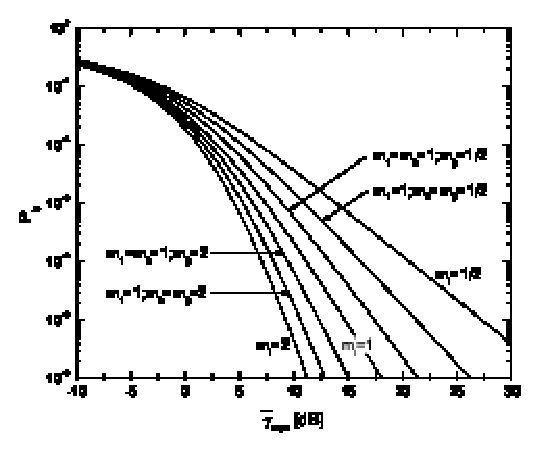
\includegraphics[width=0.6\textwidth]{grafico1}%% Dimensões e localização
\fonte{\citet{Faina2001}}%% Fonte
\end{graph}

No \autoref{gra:grafico2} é apresentado um exemplo de gráfico produzido em ``Excel''.

\begin{graph}[htb]%% Ambiente graph
%\captionsetup{width=0.6\textwidth}%% Largura da legenda
\caption{Exemplo de gráfico produzido em ``Excel''}%% Legenda
\label{gra:grafico2}%% Rótulo
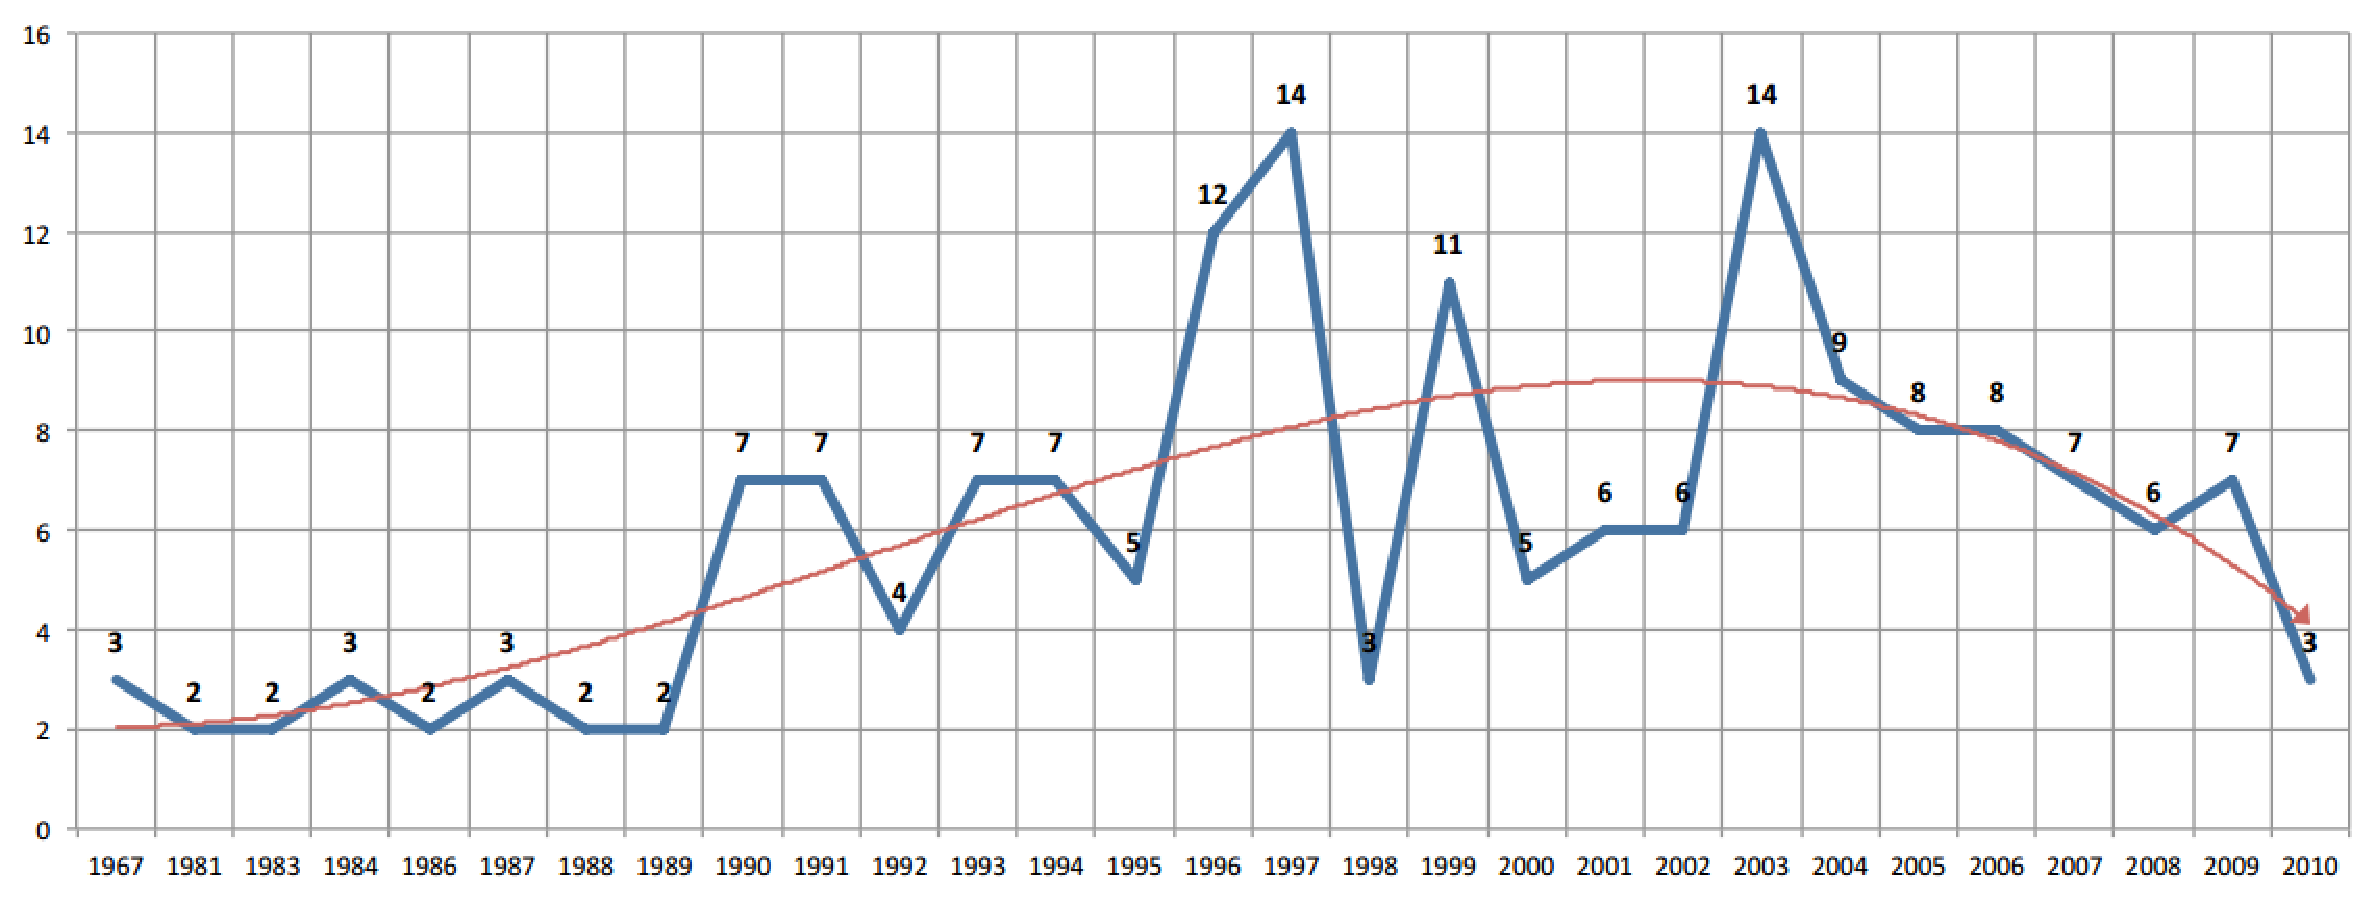
\includegraphics[width=0.6\textwidth]{grafico2}%% Dimensões e localização
\fonte{\citeonline[p. 24]{Araujo2012}}%% Fonte
\end{graph}

O ambiente \texttt{minipage} pode ser usado para inserir textos ou outros elementos em quadros com tamanhos e posições controladas, conforme exemplos apresentados no \autoref{gra:minipagegrafico1} e no \autoref{gra:minipagegrafico2}.

\begin{graph}[htb]%% Ambiente graph
\begin{minipage}[t]{0.395\textwidth}%% Ambiente minipage
\centering%% Centralizado
%\captionsetup{width=0.85\textwidth}%% Largura da legenda
\caption{Gráfico 1 do ambiente \texttt{minipage}}%% Legenda
\label{gra:minipagegrafico1}%% Rótulo
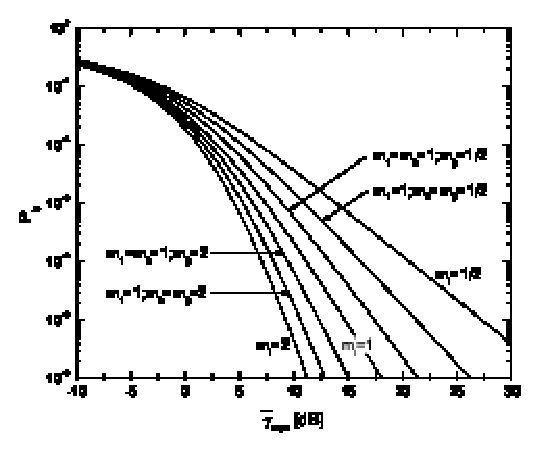
\includegraphics[width=0.85\textwidth]{grafico1}%% Dimensões e localização
\fonte{\citet{Faina2001}}%% Fonte
\end{minipage}
\hfill
\begin{minipage}[t]{0.595\textwidth}%% Ambiente minipage
\centering%% Centralizado
\captionsetup{width=0.95\textwidth}%% Largura da legenda
\caption{Gráfico 2 do ambiente \texttt{minipage}}%% Legenda
\label{gra:minipagegrafico2}%% Rótulo
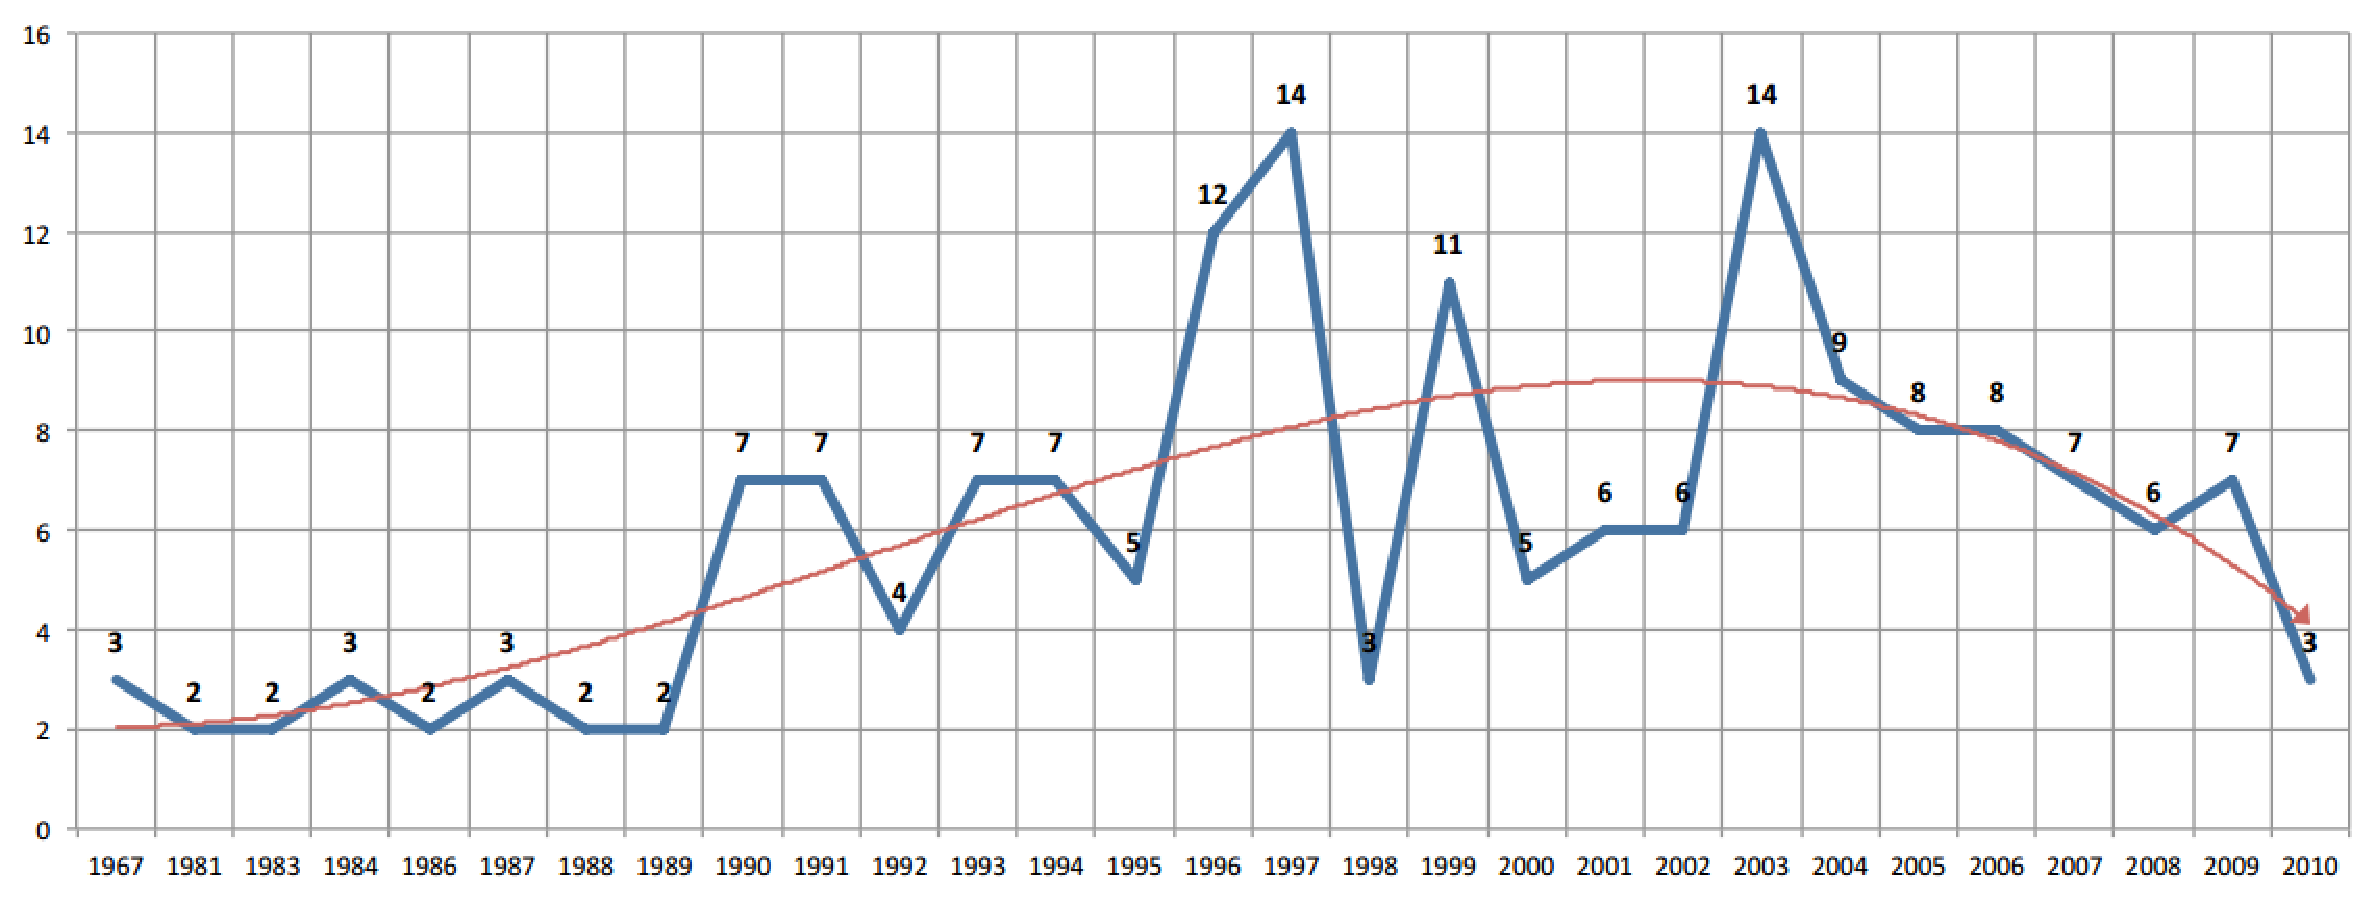
\includegraphics[width=0.95\textwidth]{grafico2}%% Dimensões e localização
\fonte{\citeonline[p. 24]{Araujo2012}}%% Fonte
\end{minipage}
\label{gra:minipagegraficos}
\end{graph}

%% Título e rótulo de seção (rótulos não devem conter caracteres especiais, acentuados ou cedilha)
\subsection{Quadros}\label{sec:quadros}

Um exemplo deste tipo de ilustração é apresentado no \autoref{quad:quadro1}.

\begin{tabframed}[htb]%% Ambiente tabframed
%\captionsetup{width=0.5\textwidth}%% Largura da legenda
\caption{Compostos orgânicos: fórmulas estruturais e principais classes}%% Legenda
\label{quad:quadro1}%% Rótulo
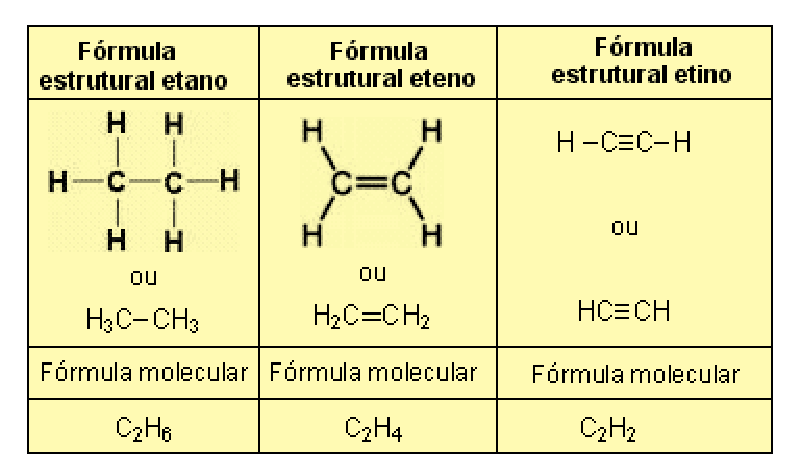
\includegraphics[width=0.5\textwidth]{quadro1}%% Dimensões e localização
\fonte{\citet{daSilva2009}}%% Fonte
\end{tabframed}

Outro exemplo deste tipo de ilustração é apresentado no \autoref{quad:quadro2}.

\begin{tabframed}[htb]%% Ambiente tabframed
%\captionsetup{width=0.7\textwidth}%% Largura da legenda
\caption{Modelos de maturidade para a gestão da cadeia de suprimentos}%% Legenda
\label{quad:quadro2}%% Rótulo
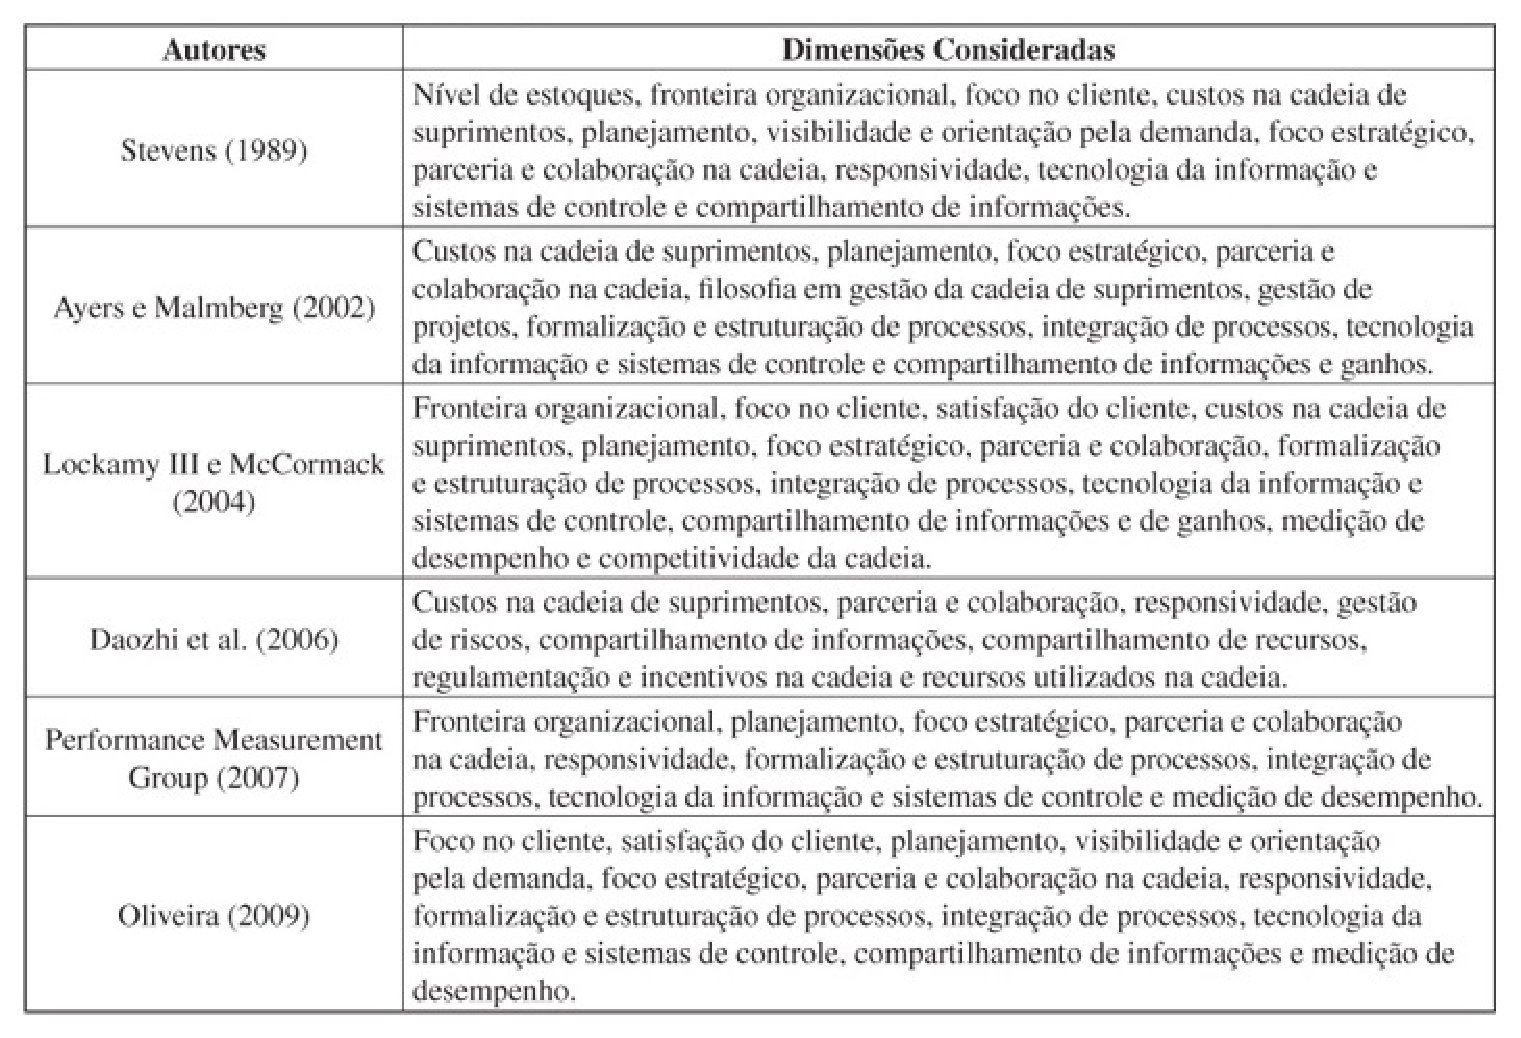
\includegraphics[width=0.7\textwidth]{quadro2}%% Dimensões e localização
\fonte{\citet{Frederico2012}}%% Fonte
\end{tabframed}

Os quadros não devem ser chamados de tabelas, uma vez que se diferenciam destas por apresentarem as laterais fechadas e o conteúdo não numérico.

%% Título e rótulo de seção (rótulos não devem conter caracteres especiais, acentuados ou cedilha)
\section{Tabelas}\label{sec:tabelas}

Tabelas são construídas com comandos próprios do \gls{latex}\index{LaTeX@\latex}. Por exemplo, a \autoref{tab:tabela1} foi construída desta forma.

\begin{table}[htb]%% Ambiente table
\caption{Primeiro exemplo de tabela com uma legenda contendo um texto muito longo que pode ocupar mais de uma linha}%% Legenda
\label{tab:tabela1}%% Rótulo
\begin{tabularx}{\textwidth}{@{\extracolsep{\fill}}llll}%% Ambiente tabularx
\toprule
$\bsym{L}$ & $\bsym{L^2}$ & $\bsym{L^3}$ & $\bsym{L^4}$ \\
\SI{}{[m]} & \SI{}{[m^2]} & \SI{}{[m^3]} & \SI{}{[m^4]} \\ \midrule
1          & 1            & 1            & 1            \\
2          & 4            & 8            & 16           \\
3          & 9            & 27           & 81           \\
4          & 16           & 64           & 256          \\
5          & 25           & 125          & 625          \\ \bottomrule
\end{tabularx}
\fonte{}%% Fonte
\end{table}

A \autoref{tab:tabela2} é um exemplo de tabela que ocupa mais de uma página e que foi construída pelo \gls{latex}\index{LaTeX@\latex} utilizando o pacote \texttt{longtable}.

\begin{longtable}{@{\extracolsep{\fill}}lll}%% Ambiente longtable
\caption{Possíveis tríplices para grade altamente variável\label{tab:tabela2}} \\%% Legenda e rótulo
\toprule
\textbf{Tempo (s)} & \textbf{Tríplice escolhida} & \textbf{Outras possíveis tríplices} \\
\midrule
\endfirsthead%% Encerra cabeçalho da primeira página
\caption[]{Possíveis tríplices para grade altamente variável} \\%% Legenda
\multicolumn{3}{r}{\textbf{(continuação)}} \\
\toprule
\textbf{Tempo (s)} & \textbf{Tríplice escolhida} & \textbf{Outras possíveis tríplices} \\
\midrule
\endhead%% Encerra cabeçalho das demais páginas
\midrule
\multicolumn{3}{r}{\textbf{(continua)}} \\
\endfoot%% Encerra rodapé das demais páginas
\bottomrule
\\[-0.5\linha]
\caption*{\nomefonte: Adaptado de \citet{Smallen2014}.} \\
\endlastfoot%% Encerra rodapé da última página
0      & (1, 11, 13725) & (1, 12, 10980), (1, 13, 8235), (2, 2, 0), (3, 1, 0) \\
2745   & (1, 12, 10980) & (1, 13, 8235), (2, 2, 0), (2, 3, 0), (3, 1, 0)      \\
5490   & (1, 12, 13725) & (2, 2, 2745), (2, 3, 0), (3, 1, 0)                  \\
8235   & (1, 12, 16470) & (1, 13, 13725), (2, 2, 2745), (2, 3, 0), (3, 1, 0)  \\
10980  & (1, 12, 16470) & (1, 13, 13725), (2, 2, 2745), (2, 3, 0), (3, 1, 0)  \\
13725  & (1, 12, 16470) & (1, 13, 13725), (2, 2, 2745), (2, 3, 0), (3, 1, 0)  \\
16470  & (1, 13, 16470) & (2, 2, 2745), (2, 3, 0), (3, 1, 0)                  \\
19215  & (1, 12, 16470) & (1, 13, 13725), (2, 2, 2745), (2, 3, 0), (3, 1, 0)  \\
21960  & (1, 12, 16470) & (1, 13, 13725), (2, 2, 2745), (2, 3, 0), (3, 1, 0)  \\
24705  & (1, 12, 16470) & (1, 13, 13725), (2, 2, 2745), (2, 3, 0), (3, 1, 0)  \\
27450  & (1, 12, 16470) & (1, 13, 13725), (2, 2, 2745), (2, 3, 0), (3, 1, 0)  \\
30195  & (2, 2, 2745)   & (2, 3, 0), (3, 1, 0)                                \\
32940  & (1, 13, 16470) & (2, 2, 2745), (2, 3, 0), (3, 1, 0)                  \\
35685  & (1, 13, 13725) & (2, 2, 2745), (2, 3, 0), (3, 1, 0)                  \\
38430  & (1, 13, 10980) & (2, 2, 2745), (2, 3, 0), (3, 1, 0)                  \\
41175  & (1, 12, 13725) & (1, 13, 10980), (2, 2, 2745), (2, 3, 0), (3, 1, 0)  \\
43920  & (1, 13, 10980) & (2, 2, 2745), (2, 3, 0), (3, 1, 0)                  \\
46665  & (2, 2, 2745)   & (2, 3, 0), (3, 1, 0)                                \\
49410  & (2, 2, 2745)   & (2, 3, 0), (3, 1, 0)                                \\
52155  & (1, 12, 16470) & (1, 13, 13725), (2, 2, 2745), (2, 3, 0), (3, 1, 0)  \\
54900  & (1, 13, 13725) & (2, 2, 2745), (2, 3, 0), (3, 1, 0)                  \\
57645  & (1, 13, 13725) & (2, 2, 2745), (2, 3, 0), (3, 1, 0)                  \\
60390  & (1, 12, 13725) & (2, 2, 2745), (2, 3, 0), (3, 1, 0)                  \\
63135  & (1, 13, 16470) & (2, 2, 2745), (2, 3, 0), (3, 1, 0)                  \\
65880  & (1, 13, 16470) & (2, 2, 2745), (2, 3, 0), (3, 1, 0)                  \\
68625  & (2, 2, 2745)   & (2, 3, 0), (3, 1, 0)                                \\
71370  & (1, 13, 13725) & (2, 2, 2745), (2, 3, 0), (3, 1, 0)                  \\
74115  & (1, 12, 13725) & (2, 2, 2745), (2, 3, 0), (3, 1, 0)                  \\
76860  & (1, 13, 13725) & (2, 2, 2745), (2, 3, 0), (3, 1, 0)                  \\
79605  & (1, 13, 13725) & (2, 2, 2745), (2, 3, 0), (3, 1, 0)                  \\
82350  & (1, 12, 13725) & (2, 2, 2745), (2, 3, 0), (3, 1, 0)                  \\
85095  & (1, 12, 13725) & (1, 13, 10980), (2, 2, 2745), (2, 3, 0), (3, 1, 0)  \\
87840  & (1, 13, 16470) & (2, 2, 2745), (2, 3, 0), (3, 1, 0)                  \\
90585  & (1, 13, 16470) & (2, 2, 2745), (2, 3, 0), (3, 1, 0)                  \\
93330  & (1, 13, 13725) & (2, 2, 2745), (2, 3, 0), (3, 1, 0)                  \\
96075  & (1, 13, 16470) & (2, 2, 2745), (2, 3, 0), (3, 1, 0)                  \\
98820  & (1, 13, 16470) & (2, 2, 2745), (2, 3, 0), (3, 1, 0)                  \\
101565 & (1, 13, 13725) & (2, 2, 2745), (2, 3, 0), (3, 1, 0)                  \\
104310 & (1, 13, 16470) & (2, 2, 2745), (2, 3, 0), (3, 1, 0)                  \\
107055 & (1, 13, 13725) & (2, 2, 2745), (2, 3, 0), (3, 1, 0)                  \\
109800 & (1, 13, 13725) & (2, 2, 2745), (2, 3, 0), (3, 1, 0)                  \\
112545 & (1, 12, 16470) & (1, 13, 13725), (2, 2, 2745), (2, 3, 0), (3, 1, 0)  \\
115290 & (1, 13, 16470) & (2, 2, 2745), (2, 3, 0), (3, 1, 0)                  \\
118035 & (1, 13, 13725) & (2, 2, 2745), (2, 3, 0), (3, 1, 0)                  \\
120780 & (1, 13, 16470) & (2, 2, 2745), (2, 3, 0), (3, 1, 0)                  \\
123525 & (1, 13, 13725) & (2, 2, 2745), (2, 3, 0), (3, 1, 0)                  \\
126270 & (1, 12, 16470) & (1, 13, 13725), (2, 2, 2745), (2, 3, 0), (3, 1, 0)  \\
129015 & (2, 2, 2745)   & (2, 3, 0), (3, 1, 0)                                \\
131760 & (2, 2, 2745)   & (2, 3, 0), (3, 1, 0)                                \\
134505 & (1, 13, 16470) & (2, 2, 2745), (2, 3, 0), (3, 1, 0)                  \\
137250 & (1, 13, 13725) & (2, 2, 2745), (2, 3, 0), (3, 1, 0)                  \\
139995 & (2, 2, 2745)   & (2, 3, 0), (3, 1, 0)                                \\
142740 & (2, 2, 2745)   & (2, 3, 0), (3, 1, 0)                                \\
145485 & (1, 12, 16470) & (1, 13, 13725), (2, 2, 2745), (2, 3, 0), (3, 1, 0)  \\
148230 & (2, 2, 2745)   & (2, 3, 0), (3, 1, 0)                                \\
150975 & (1, 13, 16470) & (2, 2, 2745), (2, 3, 0), (3, 1, 0)                  \\
153720 & (1, 12, 13725) & (2, 2, 2745), (2, 3, 0), (3, 1, 0)                  \\
156465 & (1, 13, 13725) & (2, 2, 2745), (2, 3, 0), (3, 1, 0)                  \\
159210 & (1, 13, 13725) & (2, 2, 2745), (2, 3, 0), (3, 1, 0)                  \\
161955 & (1, 13, 16470) & (2, 2, 2745), (2, 3, 0), (3, 1, 0)                  \\
164700 & (1, 13, 13725) & (2, 2, 2745), (2, 3, 0), (3, 1, 0)                  \\
\end{longtable}

Tabelas criadas em planilhas do ``Excel'' podem ser convertidas em tabelas \gls{latex}\index{LaTeX@\latex} utilizando o suplemento ``Excel-to-LaTeX'', disponível em \url{http://www.ctan.org/pkg/excel2latex}.

\textbf{Atenção!} É fortemente recomendável que as tabelas sejam criadas através de ferramentas \textit{online} ou \textit{plugins} do LibreOffice ou Microsoft Office, pois assim o trabalho de criar as tabelas fica bem mais fácil. Seguem \textit{links} de sítios \textit{online} que permitem criar tais tabelas, depois só é necessário copiar o código da tabela gerada por esses sítios para o texto do trabalho em \gls{latex}\index{LaTeX@\latex}:
\begin{itemize}
    \item \url{https://www.tablesgenerator.com/};
    \item \url{https://www.latex-tables.com/};
    \item \url{https://tableconvert.com/latex-generator};
    \item É possível buscar por outras na Internet através de termos de busca como ``latex table online'' ou ``latex criar tabela online''.
\end{itemize}

%% Título e rótulo de seção (rótulos não devem conter caracteres especiais, acentuados ou cedilha)
\section{Abreviaturas e siglas}\label{sec:acronimos}

\gls{latex}\index{LaTeX@\latex} gera automaticamente a lista de abreviaturas e siglaspor meio do pacote \texttt{glossaries}. As abreviaturas e siglas devem ser definidos no arquivo \texttt{entradas-acronimos.tex}, no diretório ``PreTexto'', com os comandos:

\begin{SingleSpacing}%% Ambiente SingleSpacing
\begin{verbatim}
\abreviatura{rótulo}{representação}{definição}
\sigla{rótulo}{representação}{definição}
\acronimo{rótulo}{representação}{definição}
\end{verbatim}
\end{SingleSpacing}

Para que a abreviatura ou sigla seja apresentada em alguma parte do texto do documento use o comando \verb|\gls{rótulo}|, por exemplo, as abreviaturas \gls{art.}, \gls{cap.} e \gls{sec.} foram geradas pelos comandos \verb|\gls{art.}, \gls{cap.} e \gls{sec.}|, respectivamente. Mais detalhes dos comandos do pacote \texttt{glossaries} podem ser encontrados em: \url{http://mirrors.ctan.org/macros/latex/contrib/glossaries/glossaries-user.pdf}.

Outra opção para gerar a lista de abreviaturas e siglas é por meio da edição manual do arquivo \texttt{lista-acronimos.tex} no diretório ``PreTexto''.

%% Título e rótulo de seção (rótulos não devem conter caracteres especiais, acentuados ou cedilha)
\section{Símbolos}\label{sec:simbolos}

\gls{latex}\index{LaTeX@\latex} gera automaticamente a lista de símbolos por meio do pacote \texttt{nomencl}. Ao redigir um símbolo pela primeira vez em qualquer parte do texto com o comando \verb|\nomenclature[prefixo]{símbolo}{descrição \nomunit{unidade}}|, é gerada uma entrada para a lista de símbolos. Veja exemplos deste comando no arquivo fonte deste capítulo. Os elementos da lista de símbolos são agrupados a depender da primeira letra atribuída ao prefixo e classificadas em:

\begin{itemize}%% Lista de itens
\item Letras Latinas.
\item Letras Gregas.
\item Sobrescritos.
\item Subscritos.
\item Notações.
\end{itemize}

Outra opção ao comando \verb|\nomenclature| é o uso dos atalhos:

\begin{SingleSpacing}%% Ambiente SingleSpacing
\begin{verbatim}
\letralatina{prefixo}{símbolo}{descrição}{unidade}
\letragrega{prefixo}{símbolo}{descrição}{unidade}
\sobrescrito{prefixo}{símbolo}{descrição}{unidade}
\subscrito{prefixo}{símbolo}{descrição}{unidade}
\notacao{prefixo}{símbolo}{descrição}{unidade}
\end{verbatim}
\end{SingleSpacing}

\noindent Neste caso a atribuição da primeira letra do prefixo pode ser desprezada.

%% Letras Latinas [A]
\nomenclature[AA]{$A$}{Área \nomunit{m^2}}%%
\letralatina{L}{L}{Comprimento}{m}%%
\letralatina{R}{R}{Raio}{m}%%
%% Letras Gregas [B]
\nomenclature[Bmu]{$\mu$}{Viscosidade dinâmica \nomunit{kg/(m.s)}}%%
\letragrega{nu}{\nu}{Viscosidade cinemática}{m^2/s}%%
\letragrega{pi}{\pi}{Pi (constante circular)}{rad}%%
\letragrega{rho}{\rho}{Massa específica}{kg/m^3}%%
\letragrega{sigma}{\sigma}{Tensão superficial}{N/m}%%
%% Sobrescritos [C]
\nomenclature[C+]{$+$}{Passo de tempo posterior}%%
\sobrescrito{-}{-}{Passo de tempo anterior}{}%%
\sobrescrito{0}{0}{Valor inicial}{}%%
%% Subscritos [D]
\nomenclature[DG]{$G$}{Fase gasosa}%%
\subscrito{L}{L}{Fase líquida}{}%%
\subscrito{S}{S}{Fase sólida}{}%%
%% Notações [E]
\nomenclature[EPsi_1]{$\overline{\Psi}$}{Média temporal}%%
\notacao{Psi_2}{\langle \Psi \rangle}{Média na seção transversal}{}%%
\notacao{Psi_3}{\langle\langle \Psi \rangle\rangle}{Média na seção transversal ponderada}{}%%

Mais detalhes dos comandos do pacote \texttt{nomencl} podem ser encontrados em: \url{http://tug.ctan.org/tex-archive/macros/latex/contrib/nomencl/nomencl.pdf}.

Outra opção para gerar a lista de símbolos é por meio da edição manual do arquivo \texttt{lista-simbolos.tex} no diretório ``PreTexto''.

%% Título e rótulo de seção (rótulos não devem conter caracteres especiais, acentuados ou cedilha)
\section{Inclusão de outros arquivos}\label{sec:inclusao}

É uma boa prática dividir o seu documento em diversos arquivos, e não apenas escrever tudo em um único. Esse recurso foi utilizado neste documento (veja \texttt{utfprpb.tex}). Para incluir diferentes arquivos em um arquivo principal, de modo que cada arquivo incluído fique em uma página diferente, utilize o comando:

\begin{SingleSpacing}%% Ambiente SingleSpacing
\begin{verbatim}
\include{documento-a-ser-incluido} %% Sem a extensão .tex
\end{verbatim}
\end{SingleSpacing}

Para incluir documentos sem quebra de páginas, utilize:

\begin{SingleSpacing}%% Ambiente SingleSpacing
\begin{verbatim}
\input{documento-a-ser-incluido}   %% Sem a extensão .tex
\end{verbatim}
\end{SingleSpacing}

%% Título e rótulo de seção (rótulos não devem conter caracteres especiais, acentuados ou cedilha)
\section{Referências}\label{sec:referencias}

A formatação das referências bibliográficas conforme as regras da \gls{abnt}\index{ABNT} são um dos principais objetivos do \gls{abntex2}\index{abnTeX2@\abnTeX}. Consulte os manuais \citeonline{abnTeX2:2013Cite} e \citeonline{abnTeX2:2013CiteAlf} para obter informações sobre sua utilização.

%% Título e rótulo de seção (rótulos não devem conter caracteres especiais, acentuados ou cedilha)
%\subsection{Acentuação de referências bibliográficas}\label{sec:acentuacaodereferencias}

Normalmente não há problemas em usar caracteres acentuados em arquivos bibliográficos (extensão \texttt{bib}). Porém, como as regras da \gls{abnt}\index{ABNT} fazem uso quase abusivo da conversão para letras maiúsculas, é preciso observar o modo como se escreve os nomes dos autores e/ou editores. No \autoref{quad:quadro3} você encontra alguns exemplos das conversões mais importantes. A regra geral é sempre usar a acentuação neste modo quando houver conversão para letras maiúsculas.

\begin{tabframed}[htb]%% Ambiente tabframed
%\captionsetup{width=0.5\textwidth}%% Largura da legenda
\caption{Conversão de acentuação em arquivos \texttt{bibtex}}%% Legenda
\label{quad:quadro3}%% Rótulo
\begin{tabular}{|*{2}{p{0.25\textwidth-\columnsep}|}}%% Ambiente tabular
\hline
\textbf{Acento}   & \textbf{Comando}                       \\ \hline
{\'a} {\`a} {\~a} & \verb|{\'a}| \verb|{\`a}| \verb|{\~a}| \\ \hline
{\^e}             & \verb|{\^e}|                           \\ \hline
{\"u}             & \verb|{\"u}|                           \\ \hline
{\'\i}            & \verb|{\'\i}|                          \\ \hline
{\c{c}}           & \verb|{\c{c}}|                         \\ \hline
\end{tabular}
\fonte{}%% Fonte
\end{tabframed}

%% Título e rótulo de seção (rótulos não devem conter caracteres especiais, acentuados ou cedilha)
\section{Glossário}\label{sec:glossario}

Você pode definir as entradas do glossário no início do texto. Recomenda-se o uso de um arquivo separado a ser inserido ainda no preâmbulo do documento, como por exemplo o arquivo \texttt{entradas-glossario.tex} no diretório ``PosTexto'' do presente documento. Veja orientações sobre inclusão de arquivos na \autoref{sec:inclusao}.

`O \gls{abntex2} é \glsdesc*{abntex2}' é um exemplo de termo definido no glossário e usado no decorrer do texto, bem como:

\begin{citacao}%% Ambiente citacao
Esta frase usa a palavra \gls{componente} e o plural de \glspl{filho}, ambas definidas no glossário como filhas da entrada \gls{pai}. \Gls{equilibrio} exemplifica o uso de um termo no início da frase. O software \gls{abntex2}\index{abnTeX2@\abnTeX} é escrito em \gls{latex}\index{LaTeX@\latex}, que é definido no glossário como `\glsdesc*{latex}'.
\end{citacao}

A frase da citação direta acima foi produzida com:

\begin{SingleSpacing}%% Ambiente SingleSpacing
\begin{verbatim}
Esta frase usa a palavra \gls{componente} e o plural de
\glspl{filho}, ambas definidas no glossário como filhas da
entrada \gls{pai}. \Gls{equilibrio} exemplifica o uso de um
termo no início da frase. O software \gls{abntex2} é
escrito em \gls{latex}, que é definido no glossário como
`\glsdesc*{latex}'.
\end{verbatim}
\end{SingleSpacing}

A impressão efetiva do glossário é dada com:

\begin{SingleSpacing}%% Ambiente SingleSpacing
\begin{verbatim}
\printglossaries
\end{verbatim}
\end{SingleSpacing}

A impressão do glossário incorpora o número das páginas em que as entradas foram citadas. Isso pode ser removido adicionando-se a opção \texttt{nonumberlist} em:

\begin{SingleSpacing}%% Ambiente SingleSpacing
\begin{verbatim}
\usepackage[nonumberlist, style=index]{glossaries}
\end{verbatim}
\end{SingleSpacing}

%% Título e rótulo de seção (rótulos não devem conter caracteres especiais, acentuados ou cedilha)
\section{Apêndices e anexos}\label{sec:apendiceseanexos}

Apêndices e anexos podem ser inseridos no documento, logo após o glossário, por meio da inclusão de arquivos, como por exemplo, os arquivos fontes \texttt{apendicea.tex}, \texttt{apendiceb.tex}, \texttt{anexoa.tex} e \texttt{anexob.tex}, presentes no diretório ``PosTexto'' deste projeto, são utilizados para gerar o \autoref{cap:apendicea}, o \autoref{cap:apendiceb}, o \autoref{cap:anexoa} e o \autoref{cap:anexob}, respectivamente. Veja orientações sobre inclusão de arquivos na \autoref{sec:inclusao}.

%% Título e rótulo de seção (rótulos não devem conter caracteres especiais, acentuados ou cedilha)
\section{Índice remissivo}\label{sec:indice}

Palavras podem ser indexadas no índice remissivo por meio do comando \verb|\index{palavra a ser indexada}|. Existem vários exemplos do uso deste comando no arquivo fonte deste capítulo. Por exemplo o comando \verb|\index{Windows}| é utilizado para indexar a palavra Windows\index{Windows} no índice remissivo.

%% Título e rótulo de seção (rótulos não devem conter caracteres especiais, acentuados ou cedilha)
\section{Compilação do documento latex}\label{sec:compilar}\index{LaTeX@\latex}

Geralmente os editores \gls{latex}\index{LaTeX@\latex}, como o TeXlipse\index{TeXlipse}\footnote{Disponível em \url{http://texlipse.sourceforge.net/}.}, o Texmaker\index{Texmaker}\footnote{Disponível em \url{http://www.xm1math.net/texmaker/}.}, entre outros, compilam os documentos automaticamente ou após configuração, de modo que você não precisa se preocupar com isto.

No entanto, você pode compilar os documentos \gls{latex}\index{LaTeX@\latex} usando os seguintes comandos, que devem ser digitados no \textit{Prompt} de comandos do Windows\index{Windows} ou no terminal do Mac\index{Mac} ou do Linux\index{Linux}:

\begin{SingleSpacing}%% Ambiente SingleSpacing
\begin{verbatim}
latex <mainfile>.tex
bibtex <mainfile>
latex <mainfile>.tex
latex <mainfile>.tex
dvips <dvips configs> <mainfile>.dvi -o <mainfile>.ps
ps2pdf <mainfile>.ps <mainfile>.pdf
\end{verbatim}
\end{SingleSpacing}

\noindent se todas as figuras no seu documento estão no formato \gls{eps}, ou então, usando os seguintes comandos:

\begin{SingleSpacing}%% Ambiente SingleSpacing
\begin{verbatim}
pdflatex <mainfile>.tex
bibtex <mainfile>
pdflatex <mainfile>.tex
pdflatex <mainfile>.tex
\end{verbatim}
\end{SingleSpacing}

\noindent se todas as figuras no seu documento estão no \gls{pdf}, ou em formatos comuns de imagens (BMP, GIF, JPG ou PNG).

%% Título e rótulo de seção (rótulos não devem conter caracteres especiais, acentuados ou cedilha)
\subsection{Problemas de compilação}\label{sec:problemas}

O \gls{utfprpbtex}\index{UTFPRPBTeX@\utfprtex} foi configurado e testado para compilar documentos \gls{latex}\index{LaTeX@\latex} sem problemas, mas por se tratar de uma linguagem de programação (para editoração) está sujeita a \textit{bugs} como qualquer outra linguagem. Além disto, o \gls{utfprpbtex}\index{UTFPRPBTeX@\utfprtex} é baseado em outras classes de documento e também utiliza uma quantidade considerável de pacotes que podem ter incompatibilidades. Portanto, alguns cuidados devem ser tomados quando se trabalha com \gls{latex}\index{LaTeX@\latex}, principalmente para novos usuários:

\begin{itemize}%% Lista de itens
\item Os comandos devem ser corretamente finalizados, ou seja, deve-se verificar a abertura e fechamento dos colchetes e chaves: \verb|\comando[opções]{argumentos}|. Alguns comandos não necessitam disto, por exemplo \verb|\comando|, mas as vezes torna-se necessário colocar uma barra invertida, \verb|\|, ou chaves, \verb|{}|, após o comando para gerar um espaço com o texto na sequência: \verb|\comando\ texto na sequência do comando| ou \verb|\comando{} texto na sequência do comando|.
\item Os ambientes devem ser corretamente finalizados, ou seja, deve-se verificar a abertura e fechamento dos ambientes: \verb|\begin{ambiente} ... \end{ambiente}|.
\item Os caracteres especiais devem ser precedidos de barra invertida quando se deseja imprimí-los no texto: \verb|\$ \& \% \# \_ \{ \}| resulta em \$ \& \% \# \_ \{ \}. Do contrário, não serão impressos e executarão comandos específicos do \gls{latex}\index{LaTeX@\latex}.
\item Os textos copiados de outros arquivos (\texttt{*.doc}, \texttt{*.html}, \texttt{*.pdf}, etc.) para os arquivos fonte do \gls{latex}\index{LaTeX@\latex} (\texttt{*.tex}, \texttt{*.bib}, etc.) devem ter a mesma codificação de caracteres (\texttt{UTF8}). Do contrário, alguns caracteres não serão devidamente impressos ou causarão erro, por exemplo, o hífen e os caracteres acentuados.
\item Os nomes de arquivos carregados no modelo (arquivos fontes, figuras, etc.) não devem conter caracteres especiais ou acentuados: \verb|capitulo1.tex| ao invés de \verb|capitulo_1.tex|. Esta regra também se aplica aos rótulos: \verb|\label{cap:capitulo1}| ao invés de \verb|\label{cap:capitulo_1}|.
\end{itemize}

Outras dicas de uso dos comandos do \gls{latex}\index{LaTeX@\latex} podem ser encontradas em diversos materiais de referência disponíveis na Internet, por exemplo: \url{http://en.wikibooks.org/wiki/LaTeX}, \url{http://repositorios.cpai.unb.br/ctan/info/lshort/portuguese-BR/lshortBR.pdf}, entre outros.

%% Licença utilizada no trabalho da UTFPR
\section{Licença}\label{sec:licenca}

De acordo com a Resolução Conjunta \href{https://sei.utfpr.edu.br/sei/publicacoes/controlador_publicacoes.php?acao=publicacao_visualizar&id_documento=1811618&id_orgao_publicacao=0}{nº 01/2020 COGEP-COPPG}, os trabalhos de conclusão de curso da \gls{utfpr} devem adotar uma licença Creative Commons, sendo que o texto das possíveis licenças pode ser visto em: \url{https://creativecommons.org/licenses/?lang=pt_BR}.

Para facilitar a adoção dessas licenças o presente \textit{template} possui o comando \texttt{$\backslash$licenca\{\}}, disponível no arquivo \texttt{variaveis.tex} do \textit{template}. As possibilidades para este comando são:

\begin{itemize}
    \item \texttt{$\backslash$licenca\{ccby\}} - para usar a licença CC BY (está como padrão no \textit{template}); 
    \item \texttt{$\backslash$licenca\{ccbysa\}} - para usar a licença CC BY CA;
    \item \texttt{$\backslash$licenca\{ccbynd\}} - para usar a licença CC BY ND;
    \item \texttt{$\backslash$licenca\{ccbync\}} - para usar a licença CC BY NC;
    \item \texttt{$\backslash$licenca\{ccbyncsa\}} - para usar a licença CC BY NC SA;
    \item \texttt{$\backslash$licenca\{ccbyncnd\}} - para usar a licença CC BY NC ND;
    \item \texttt{$\backslash$licenca\{\}} - deixar em branco, neste caso não aparecerá nenhuma licença (não recomendável).
\end{itemize}

Então, converse com o orientador a respeito de qual licença utilizar, localize o comando \texttt{$\backslash$licenca\{\}} no arquivo \texttt{variaveis.tex} e deixe descomentado (sem o \texttt{\%} no inicio da linha) apenas a licença que será utilizada no trabalho. Atenção, tome o cuidado de não deixar mais de uma licença desabilitada e confira se a licença escolhida é a que está aparecendo na Folha de Rosto do trabalho.%% Comente para remover este item

%% Parte
% \part{Conclusão}%% Comente para remover este item

%% Capítulo
% %%%% CAPÍTULO 5 - CONCLUSÕES E PERSPECTIVAS
%%
\chapter{Conclusão}\label{cap:conclusoeseperspectivas}

Inicia com um resumo do trabalho, retomando o(s) objetivo(s), o referencial teórico e o uso das ferramentas e das tecnologias utilizadas no trabalho.

A conclusão contém a opinião do autor em relação às vantagens, desvantagens, facilidades e limitações das tecnologias e/ou do método utilizados, as dificuldades encontradas e como foram superadas.

Também devem ser apresentadas as vantagens, desvantagens e limitações do trabalho desenvolvido, sempre tendo em vista a sua contribuição para a comunidade acadêmica e profissional e para a sociedade como um todo.

É a opinião técnica do autor do trabalho em relação ao assunto sob a forma de uma espécie de avaliação em relação ao trabalho desenvolvido e as tecnologias utilizadas.

Finaliza verificando se o objetivo foi alcançado e com a opinião do autor sobre o assunto, de acordo com o referencial teórico e com os resultados obtidos.

As perspectivas futuras são opcionais, devem ser apresentadas somente caso o acadêmico pretenda dar continuidade ao trabalho, ou mesmo se ele julgar relevante que outras pessoas dêem continuidade ao seu trabalho.
%% Comente para remover este item

%% Capítulos após este comando criam marcadores do pdf na raiz
% \phantompart%% Comente para remover este item


%% Formatação de páginas de elementos pós-textuais
\postextual%% Não comente esta linha

%% Arquivos de referências
\arquivosdereferencias{%% Arquivos bibtex sem a extensão .bib e separados por vírgula - Não comente esta linha
  %./PosTexto/exemplos-referencias,%% Arquivo de referências - Comente para remover este item
  main%% Arquivo de referências - Comente para remover este item
}%% Não comente esta linha

%% Glossário
%\incluirglossario %% Comente para remover este item

%% Arquivos de apêndices
 \begin{arquivosdeapendices}%% Os arquivos de apêndices devem se incluídos neste ambiente - Não comente esta linha
%   %\partapendices%% Página de início dos apêndices - adiciona uma página com o título Apêndices
%   %% Capítulo de exemplo
   %%%%% APÊNDICE A
%%
%% Texto ou documento elaborado pelo autor, a fim de complementar sua argumentação, sem prejuízo da unidade nuclear do trabalho.

%% Título e rótulo de apêndice (rótulos não devem conter caracteres especiais, acentuados ou cedilha)
\chapter{Questionário de pesquisa}\label{cap:apendicea}

Quando houver necessidade pode-se apresentar como apêndice documento(s) auxiliar(es) e/ou complementar(es) como: legislação, estatutos, gráficos, tabelas, etc. Os apêndices são enumerados com letras maiúsculas: \autoref{cap:apendicea}, \autoref{cap:apendiceb}, etc.

No \latex\ apêndices são editados como capítulos. O comando \verb|\appendix| faz com que todos os capítulos seguintes sejam considerados apêndices.

Apêndices complementam o texto principal da tese com informações para leitores com especial interesse no tema, devendo ser considerados leitura opcional, ou seja, o entendimento do texto principal da tese não deve exigir a leitura atenta dos apêndices.

Apêndices usualmente contemplam provas de teoremas, deduções de fórmulas matemáticas, diagramas esquemáticos, gráficos e trechos de código. Quanto a este último, código extenso não deve fazer parte da tese, mesmo como apêndice. O ideal é disponibilizar o código na Internet para os interessados em examiná-lo ou utilizá-lo.

%% Título e rótulo de seção (rótulos não devem conter caracteres especiais, acentuados ou cedilha)
%\section{Título da Seção Secundária do Apêndice B}\label{sec:secaoapendicea}

%Exemplo de seção secundária em apêndice (\autoref{sec:secaoapendicea} do \autoref{cap:apendicea}).

%% Título e rótulo de seção (rótulos não devem conter caracteres especiais, acentuados ou cedilha)
%\subsection{Título da Seção Terciária do Apêndice B}\label{subsec:subsecaoapendicea}

%Exemplo de seção terciária em apêndice (\autoref{subsec:subsecaoapendicea} do \autoref{cap:apendicea}).

%% Título e rótulo de seção (rótulos não devem conter caracteres especiais, acentuados ou cedilha)
%\subsubsection{Título da seção quaternária do Apêndice B}\label{subsubsec:subsubsecaoapendicea}

%Exemplo de seção quaternária em apêndice (\autoref{subsubsec:subsubsecaoapendicea} do \autoref{cap:apendicea}).

%% Título e rótulo de seção (rótulos não devem conter caracteres especiais, acentuados ou cedilha)
%\paragraph{Título da seção quinária do Apêndice B}\label{para:paragraphapendicea}

%Exemplo de seção quinária em apêndice (\autoref{para:paragraphapendicea} do \autoref{cap:apendicea}).
%% Apêndice - Comente para remover este item
   %%%%% APÊNDICE B
%%
%% Texto ou documento elaborado pelo autor, a fim de complementar sua argumentação, sem prejuízo da unidade nuclear do trabalho.

%% Título e rótulo de apêndice (rótulos não devem conter caracteres especiais, acentuados ou cedilha)
\chapter{Roteiro da entrevista}\label{cap:apendiceb}

\begin{table}[htb]%% Ambiente table
\caption{Orçamento dos materiais n.\textsuperscript{o} 1.}%% Legenda
\label{tab:tab3}%% Rótulo
\begin{tabularx}{\textwidth}{@{\extracolsep{\fill}}lrrr}%% Ambiente tabularx
\toprule
Material              & \multicolumn{1}{c}{Valor (R\$)} & \multicolumn{1}{c}{Quantidade}  & \multicolumn{1}{c}{Total (R\$)} \\ \midrule
Bomba centrífuga      & 2500,00                         & 01                              & 2500,00                         \\
Compressor rotativo   & 3000,00                         & 01                              & 3000,00                         \\
Manômetro diferencial & 450,00                          & 02                              & 900,00                          \\
Termopar              & 370,00                          & 02                              & 740,00                          \\
Válvula de esfera     & 43,00                           & 02                              & 86,00                           \\
Tubulação de PVC      & 10,00                           & 05                              & 50,00                           \\
Conexão de PVC        & 5,00                            & 10                              & 50,00                           \\ \midrule
                      &                                 & \multicolumn{1}{r}{Total (R\$)} & 7326,00                         \\ \bottomrule
\end{tabularx}
\fonte{}%% Fonte
\end{table}

\begin{table}[htb]%% Ambiente table
\caption{Orçamento dos materiais n.\textsuperscript{o} 2.}%% Legenda
\label{tab:tab4}%% Rótulo
\begin{tabularx}{\textwidth}{@{\extracolsep{\fill}}lrrr}%% Ambiente tabularx
\toprule
Material              & \multicolumn{1}{c}{Valor (R\$)} & \multicolumn{1}{c}{Quantidade}  & \multicolumn{1}{c}{Total (R\$)} \\ \midrule
Bomba centrífuga      & 2700,00                         & 01                              & 2700,00                         \\
Compressor rotativo   & 2950,00                         & 01                              & 2950,00                         \\
Manômetro diferencial & 515,00                          & 02                              & 1030,00                         \\
Termopar              & 350,00                          & 02                              & 700,00                          \\
Válvula de esfera     & 40,00                           & 02                              & 80,00                           \\
Tubulação de PVC      & 8,00                            & 05                              & 40,00                           \\
Conexão de PVC        & 6,00                            & 10                              & 60,00                           \\ \midrule
                      &                                 & \multicolumn{1}{r}{Total (R\$)} & 7560,00                         \\ \bottomrule
\end{tabularx}
\fonte{}%% Fonte
\end{table}

\begin{table}[htb]%% Ambiente table
\caption{Orçamento dos materiais n.\textsuperscript{o} 3.}%% Legenda
\label{tab:tab5}%% Rótulo
\begin{tabularx}{\textwidth}{@{\extracolsep{\fill}}lrrr}%% Ambiente tabularx
\toprule
Material              & \multicolumn{1}{c}{Valor (R\$)} & \multicolumn{1}{c}{Quantidade}  & \multicolumn{1}{c}{Total (R\$)} \\ \midrule
Bomba centrífuga      & 2600,00                         & 01                              & 2600,00                         \\
Compressor rotativo   & 3100,00                         & 01                              & 3100,00                         \\
Manômetro diferencial & 500,00                          & 02                              & 1000,00                         \\
Termopar              & 400,00                          & 02                              & 800,00                          \\
Válvula de esfera     & 45,00                           & 02                              & 90,00                           \\
Tubulação de PVC      & 12,00                           & 05                              & 60,00                           \\
Conexão de PVC        & 5,00                            & 10                              & 50,00                           \\ \midrule
                      &                                 & \multicolumn{1}{r}{Total (R\$)} & 7700,00                         \\ \bottomrule
\end{tabularx}
\fonte{}%% Fonte
\end{table}
%% Apêndice - Comente para remover este item
 \end{arquivosdeapendices}%% Não comente esta linha


% \begin{apendicesenv}%% Ambiente apendicesenv

% \partapendices
% \chapter{Ola}

% \lipsum[55-56]

% \end{apendicesenv}

%% Arquivos de anexos
\begin{arquivosdeanexos}%% Os arquivos de anexos devem se incluídos neste ambiente - Não comente esta linha
  %\partanexos%% Página de início dos anexos - adiciona uma página com o título Anexos

  %%%%% ANEXO A
%%
%% Texto ou documento não elaborado pelo autor, que serve de fundamentação, comprovação e ilustração.

%% Título e rótulo de anexo (rótulos não devem conter caracteres especiais, acentuados ou cedilha)
\anexos
\chapter{Lei N\texorpdfstring{.\textsuperscript{o}}{o.} 9.610, de 19 de Fevereiro de 1998}\label{cap:anexoa}

\centerline{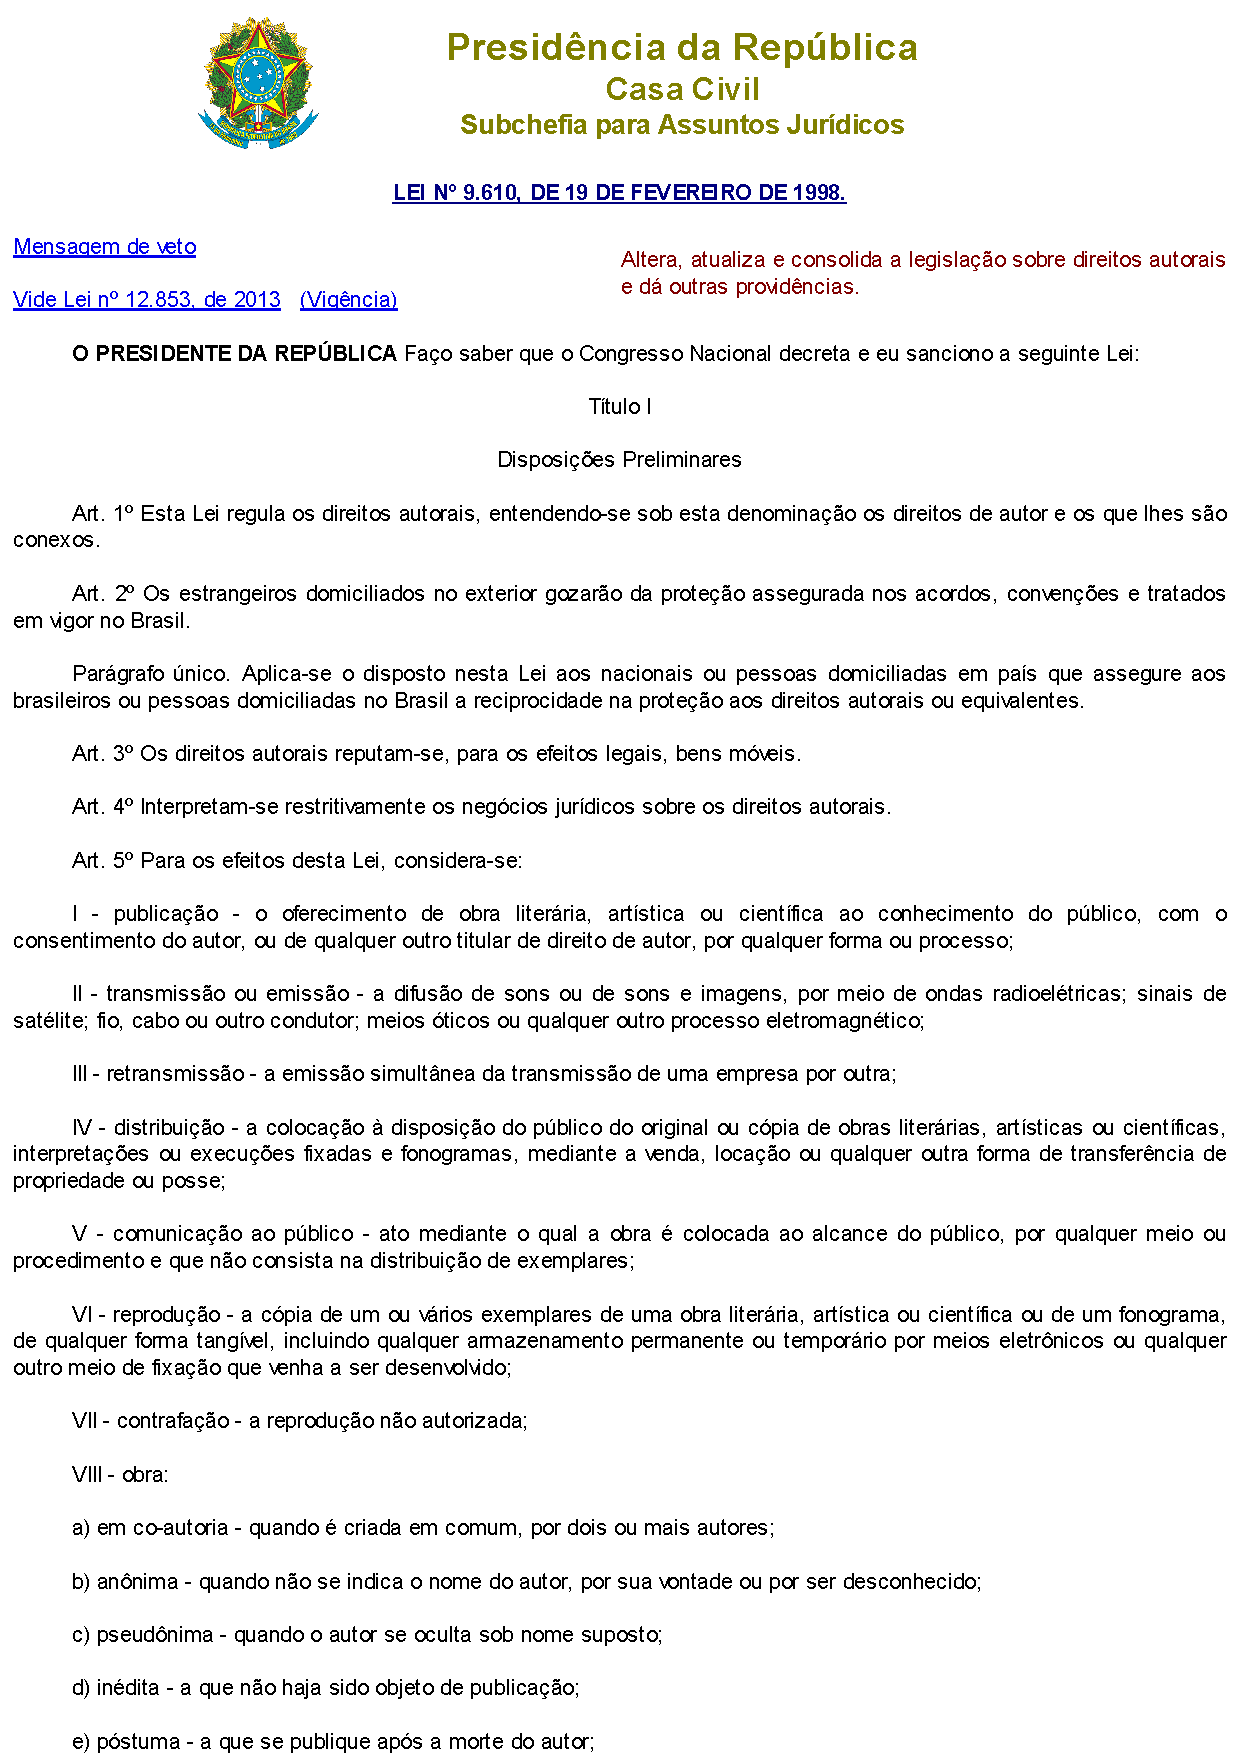
\includegraphics[width=\textwidth]{./PosTexto/Ilustracoes/lei-n9610-p1}}%% Imagem (Dimensões e localização)

\centerline{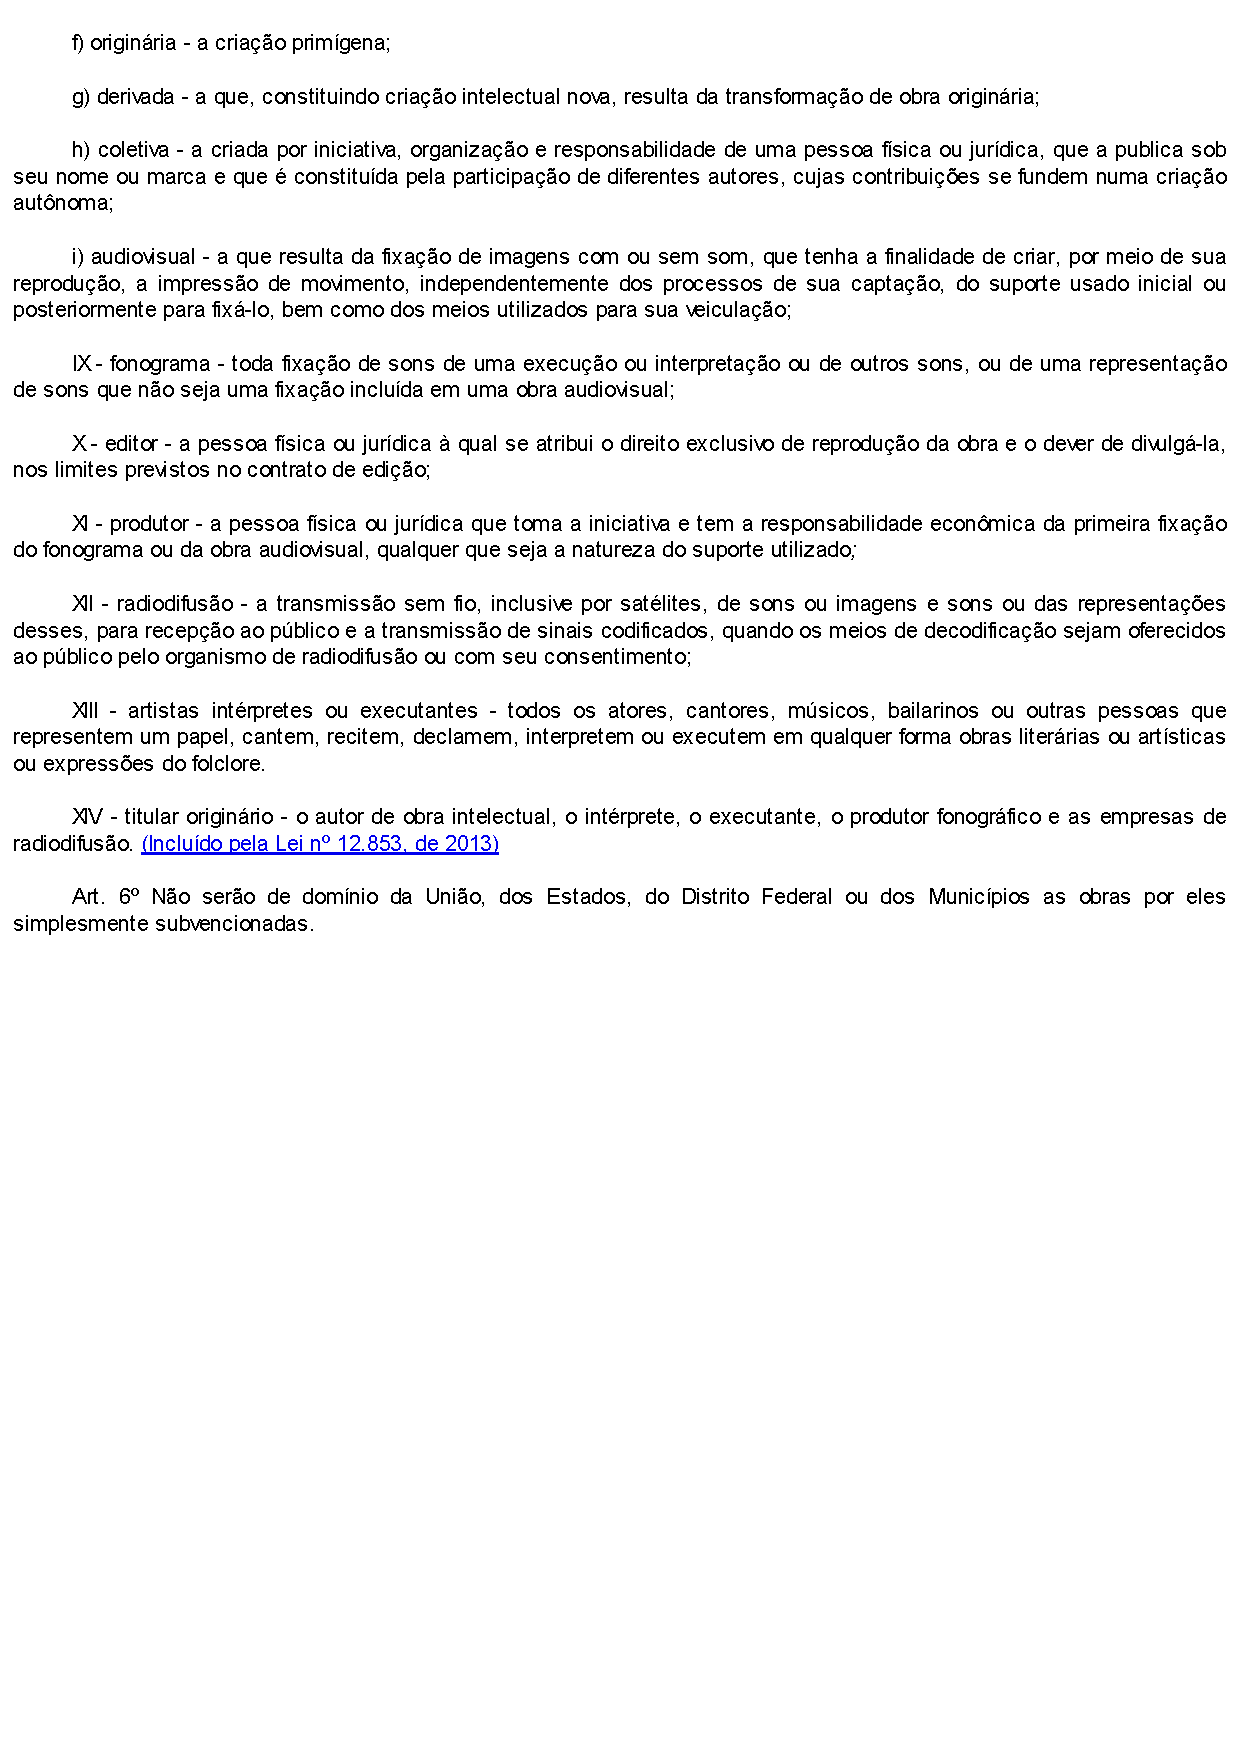
\includegraphics[width=\textwidth]{./PosTexto/Ilustracoes/lei-n9610-p2}}%% Imagem (Dimensões e localização)
%% Anexo - Comente para remover este item
  %%%%% ANEXO B
%%
%% Texto ou documento não elaborado pelo autor, que serve de fundamentação, comprovação e ilustração.

%% Título e rótulo de anexo (rótulos não devem conter caracteres especiais, acentuados ou cedilha)
\chapter{Normas para elaboração de trabalhos acadêmicos}\label{cap:anexob}

As normas da \gls{utfpr} podem ser acessadas em: \url{http://portal.utfpr.edu.br/biblioteca/trabalhos-academicos/discentes/orientacao-para-trabalhos-academicos}. Ver Figura \ref{fig:capadolivro}.

\begin{figure}[htb]%% Ambiente figure
\captionsetup{width=0.9\textwidth}%% Largura da legenda
\caption{Sítio: Normas para Elaboração de Trabalhos Acadêmicos.}%% Legenda
\label{fig:capadolivro}%% Rótulo
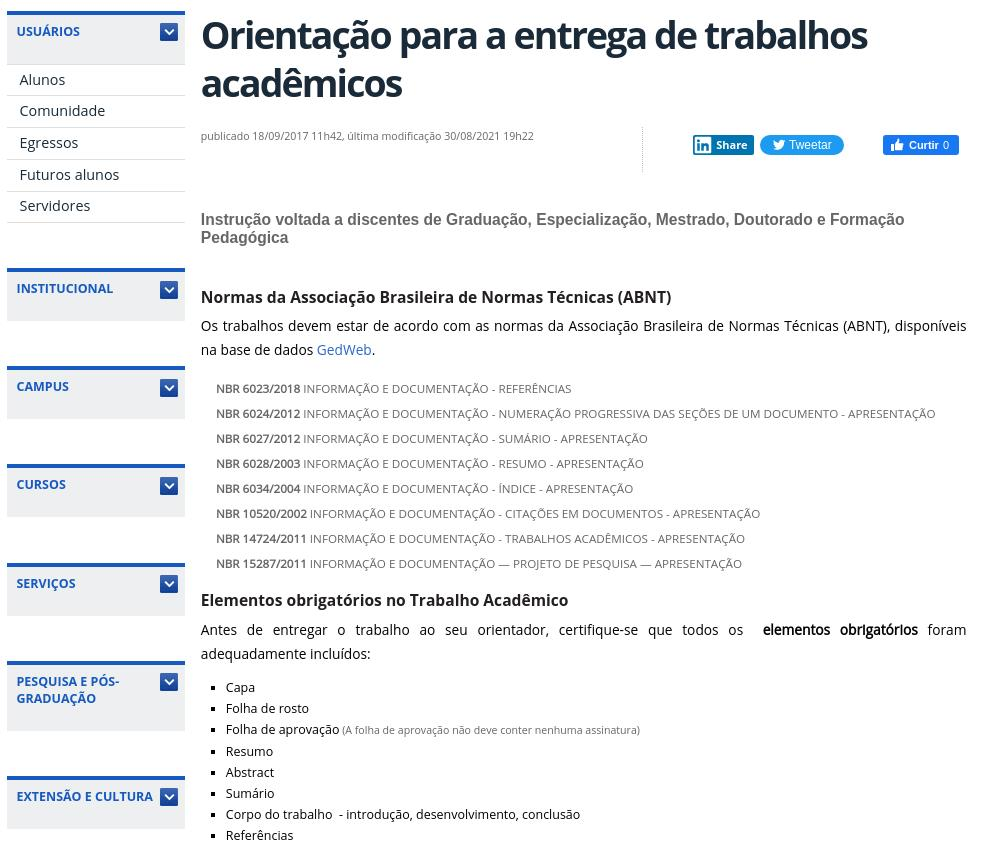
\includegraphics[width=0.9\textwidth]{normas}%% Dimensões e localização
\fonte{\cite{UTFPR2008}}%% Fonte
\end{figure}

%% Anexo - Comente para remover este item
\end{arquivosdeanexos}%% Não comente esta linha

%% Índice - Adiciona um índice remissivo.
%\incluirindice%% Comente para remover este item

%% Fim do documento
\end{document}%% Não comente esta linha
